\documentclass{ffhsthesis}

\usepackage{silence}

\WarningFilter{hyperref}{You have enabled option `breaklinks'.}

\usepackage[utf8]{inputenc}
\usepackage[ngerman]{babel}
\usepackage[table,xcdraw]{xcolor}
\usepackage[colorlinks=true, allcolors=blue]{hyperref}
\usepackage[automark,headsepline]{scrlayer-scrpage}
\usepackage[setspace=false]{scrhack}

\usepackage{bm,cite,fontawesome5,microtype,enumitem,amsmath,svg,amssymb,afterpage,caption,tabto,minted,mdframed,url,tcolorbox,blindtext,mathrsfs,pdflscape,thmtools,todonotes,subcaption,csquotes,tabularx,adjustbox,float}

\setkomafont{caption}{\footnotesize\itshape}
\setkomafont{captionlabel}{\usekomafont{caption}}
\newenvironment{code}{\captionsetup{type=listing}}{}
\renewcommand{\sectionmark}[1]{\markright{#1}}
\setkomafont{pagehead}{\normalfont\normalcolor}

\MakeOuterQuote{"}

% Keywords command
\providecommand{\keywords}[1]
{
  \small	
  \textbf{\textit{Keywords---}} #1
}

\declaretheorem{theorem}
\declaretheorem[sibling=theorem]{lemma}

\numberwithin{equation}{chapter}

\graphicspath{ {./images/} }

\definecolor{LightGray}{gray}{0.9}

\TabPositions{4cm}

\begin{document}

\dokumentTyp{Bachelor-Thesis}
\studiengang{Informatik}
\title{Quantitative Analyse von Netzwerk-Massen}
\subtitle{Usefulness und weitere Aspekte} % optional
\titelbild[height=5cm]{images/title_image}  % optional
\author{Luca Hostettler}
\date{15. März 2023}
\wohnort{Zürich}
\referent{Ao. Prof. Dr. habil. Matthias Dehmer\\ Departement Informatik\\Dozent Data Science}
% \referentin{Name des/der Referenten/in\\ Titel\\Dozent:in für Fach}
\eingereichtBei{Prof. Dr. Tobias Häberlein\\ Departement Informatik\\Departementsleiter}

\dedication{
  \textit{Diese Arbeit widme ich meiner Familie und meiner Partnerin Nathalie, welche stets an meiner Seite standen und mich unterstützt haben. Ohne ihre Hilfe wäre dies nicht möglich gewesen} \faHeart.

  \textit{Mein Dank gilt meinem Betreuer Prof. Dr. Matthias Dehmer, welcher mich vor 2 Jahren in den Bereich der Graphentheorie eingeführt hat und mir diese spannenden Reise ermöglicht hat.}

  \textit{Ebenso bedanken will ich mich bei Marc, ein Sparringpartner grosser Klasse und ein wahrer Freund} \faHandshake!
}

\maketitle

\begin{zusammenfassung}

    In diesem Forschungsprojekt wurden nützliche topologische Indizes für bestimmte Klassen und Strukturen von Graphen im Bereich der Graphentheorie untersucht.
    Durch die Berechnung diverser Indizes für eine Reihe von Graphen und den Vergleich ihrer Leistung wurde in der Studie ermittelt, welche Indizes für verschiedene Graphenklassen am nützlichsten sind. \\
    Auf der Grundlage dieser Erkenntnisse wurde eine Anwendung entwickelt, die anhand eines Eingabegraphen den einflussreichsten topologischen Index für die jeweilige Klasse bestimmt.
    Diese Anwendung hat das Potenzial, ein wertvolles Werkzeug für Forscher und Praktiker zu sein, die mit Graphdaten arbeiten, und könnte für ein breites Spektrum eingesetzt werden, darunter molekulare, bioinformatische, soziale und synthetische Graphen. \\
    Insgesamt bieten die Ergebnisse dieser Studie wesentliche Einblicke in die Verwendung von topologischen Indizes in der Graphenanalyse und können Forschung und Praxis in diesem Bereich potenziell beeinflussen.

\end{zusammenfassung}

\keywords{Graphentheorie, Topologische Indizes, Statistische Analyse, Graphenklassifikation}

\newpage

\begin{abstract}

    This thesis presents the findings of a comprehensive study on the usefulness of topological indices for specific classes and structures of graphs in graph theory.
    Using a variety of graphs, including molecular, bioinformatics, social, and synthetic graphs, this study calculated a range of topological indices and compared their performance on each graph class.  \\
    The results indicated that different indices had varying degrees of influence on the principal components of graph classes, with some indices being more useful than others for particular classes of graph. \\
    Based on these findings, the study developed an application that classifies an input graph into one of the four graph classes. The application then returns the most influential topological index for the given class, as determined by the results of the principal component analysis. The findings of this study have significant implications for the use of topological indices in a wide range of applications and provide valuable insights for researchers and practitioners working with graph data.

\end{abstract}

\keywords{Graph theory, Comparative analysis, Topological indices, Principal component analysis, Graph classification}


\tableofcontents

\begin{abkuerzungen}[MUSTER] % Das Muster dient zur Bestimmung der Einrueckungstiefe
  \item[BioChem] Biochemie
  \item[ChemInf] Chemieinformatik
  \item[CNN] Convolutional Neural Network
  \item[DB] Database
  \item[DGCNN] Deep Graph Convolutional Neural Network
  \item[FFHS] Fernfachhochschule Schweiz
  \item[GCN] Graph Convolutional Network
  \item[GNN] Graph Neural Network
  \item[PC] Principal Component
  \item[PCA] Principal Component Analysis
  \item[QSAR] Quantitative Structure-Activity Relationship
  \item[QSPR] Quantitative Structure-Property Relationship
  \item[SVM] Support Vector Machine
  \item[WWW] World Wide Web 
\end{abkuerzungen}

\clearpairofpagestyles
\cfoot[\pagemark]{\pagemark}
\ihead{\leftmark}
\ohead{\rightmark}
\pagestyle{scrheadings}

\startThesis % Befehl muss vor dem ersten chapter stehen (Seitennummerierung!)

\chapter{Einleitung} \label{chap:introduction}

Die Netzwerktheorie ist ein untergeordnetes Forschungsfeld der Mathematik und Data Science.
Seit über 80 Jahren wird im akademischen Bereich der Graphentheorie aktiv geforscht \cite{kozyrev_graph_1974,bavelas_alex_1948}.
Kozyrev fasst in seiner Analyse von 1974 die bedeutendsten Meilensteine in der Vergangenheit der Netzwerktheorie zusammen.
Weiter diskutiert er über deren Ursprung und verweist dabei auf Euler’s, die berühmten \enquote{sieben Brücken von Königsberg} aus dem Jahr 1726.

Im Jahr 1977, also drei Jahre nach Kozyrevs Veröffentlichung, ist ein Artikel von Linton Freeman erschienen, in welchem dieser die Zentralitätsmasse eines Netzes auf Basis der Forschung von Bavelas definiert \cite{freeman_set_1977,bavelas_alex_1948}.
Über die Jahre sind zahlreiche Masse entwickelt worden, um die Struktur von Netzwerken zu analysieren, wie der Wiener-Index \cite{wiener_structural_1947} oder der Randić-Index \cite{randic_characterization_1975}.
Bei den Massen geht es darum, die Struktur eines Netzwerkes zu charakterisieren oder einzigartige Muster in Netzen zu erkennen. In den darauffolgenden Jahren sind immer mehr Masse veröffentlicht worden.
Mit der Zeit wird es kompliziert, für ein Netzwerk die richtigen Masse zu finden, welche eine kräftige Aussage über dessen Topologie geben.

\section{Herleitung}

Von Balaban et al. \cite{balaban_1983_2014} werden über 1983 topologische Netzwerkindizes zusammengefasst.
Viele davon eignen sich nicht für alle Netzwerkklassen und einige überschneiden sich mit anderen \cite{balaban_highly_1982,kraus_probabilistic_2014,gomes_combination_2019}.
Je nach Betrachtung gibt es sogar Redundanzen von bestimmten Massen.

\subsection{Stand der Forschung}

Der Begriff \enquote{Usefulness} ist in der Graphentheorie ausgesprochen schwer zu definieren \cite[p.~144]{ma_usefulness_2022}, es gibt aber verschiedene anwendungsspezifische Ansätze, wie die \enquote{Usefulness} eines Messwertes definiert werden kann \cite[p.~932]{basak_qspr_2000} \cite[p.~581]{raychaudhury_discrimination_1984}.
Es wird beabsichtigt, die Usefulness von topologischen Indizes in einer quantitativen Studie von vordefinierten Netzwerkklassen zu untersuchen.
Diese Arbeit wird sich auf einzelne topologische Indizes konzentrieren und ihre Korrelation und Ähnlichkeit innerhalb der Netzwerkklassen analysieren.

\subsubsection{Die Suche nach dem optimalen Index}

Bereits im Jahr 1990 forschte Randić nach den optimalen Indizes \cite{randic_croatica_nodate}.
In einer Ausgabe der Croatia Chemica Acta dokumentiert er die Suche nach einem optimalen Mass, welches die Eigenschaften eines Graphen am ausführlichsten beschreibt.
Die kritische Feststellung von Randić ist, dass die topologischen Indizes möglichst orthogonal sein sollten, um die Eigenschaften eines Graphen am besten wiederzugeben \cite{randic_croatica_nodate}.
Aus den Ergebnissen ist ersichtlich, dass bestimmte topologische Indizes sich besser eignen, bestimmte Eigenschaften vorherzusagen, während andere weniger effektiv sind. 
Randić schlussfolgert, dass eine Kombination von Indizes die besten Vorhersagen ermöglicht und dass die Suche nach dem optimalen Set von Indizes ein wesentlicher Schritt bei der Vorhersage von Moleküleigenschaften ist.
Es konnte bereits festgestellt werden, dass verschiedene Masse eine gewisse Redundanz aufweisen \cite{kraus_probabilistic_2014}. 

\subsubsection{Usefulness}

\paragraph{Usefulness-Score}

Der Usefulness-Score (engl. für Nützlichkeitspunktzahl) ist ein Mass dafür, wie nützlich oder hilfreich etwas ist.
Er wird häufig verwendet, um Produkte, Dienstleistungen oder Informationsquellen zu bewerten und deren Wirksamkeit zu bestimmen.
Es gibt zahlreiche Möglichkeiten, Nützlichkeitsbewertungen zu berechnen.

Die spezifische Methode, die eingesetzt wird, hängt dabei vom gegebenen Kontext ab, für den die Bewertung dient.
Einige gängige Methoden sind Kundenbefragungen, Benutzertests und Expertenbewertungen.
Beispielsweise kann ein Unternehmen Kunden befragen, um die Nützlichkeit seiner Produkte zu ermitteln, oder ein Forscher kann Benutzertests durchführen, um die Nützlichkeit einer neuen Softwareanwendung zu bewerten.
Mit Usefulness-Scores kann die Entscheidungsfindung in einer Vielzahl von Kontexten quantifiziert werden.
Ein Unternehmen kann etwa über Kundenfeedback und Nützlichkeitsbewertungen bestimmen, welche Produkte auf Lager gehalten werden sollen oder ob Verbesserungen an bestehenden Produkten vorzunehmen sind. 
In ähnlicher Weise kann eine Bibliothek Usability-Studien und Usefulness-Scores verwenden, um zu ermitteln, welche Ressourcen gekauft oder Benutzern zur Verfügung gestellt werden sollen \cite{fiszman_automatic_2009}.

\paragraph{Usefulness von topologischen Indizes}

In derselben Arbeit von Randić (1990) \cite{randic_croatica_nodate} werden \textit{nützliche} Eigenschaften von topologischen Indizes angesprochen.
Danail Bonchev und Oskar E. Polansky diskutieren die Anwendung von Konzepten wie Knoten- und Graphentheorie auf chemische Strukturen und zeigen, wie sie zur Beschreibung von Eigenschaften wie Reaktivität und Stabilität von Verbindungen verwendet werden können. 
Bonchev argumentiert, dass topologische Indizes eine effektive Möglichkeit darstellen, komplexe chemische Systeme zu beschreiben und zu verstehen sowie, dass ihre Verwendung bei der Vorhersage und Modellierung chemischer Reaktionen von grossem Nutzen sein kann \cite{bonchev_topological_1987}.

\paragraph{Genereller Ansatz zur Usefulness}

Von Ma et al. \cite{ma_usefulness_2022} wurden erste Versuche unternommen, um Messwerte für verschiedene Klassen zu bewerten und deren Usefulness zu berechnen.
Im dazu in der Zeitschrift Information Sciences veröffentlichten Artikel \cite{ma_usefulness_2022} wird ein topologischer Index als numerisches Mass definiert, das die topologische Struktur eines Graphen charakterisiert und dazu verwendet werden kann, um die Konnektivität oder Komplexität eines Netzwerks zu beschreiben. 
In ihrer Veröffentlichung legen die Wissenschaftler die Nutzung topologischer Indizes in einer Vielzahl von Bereichen dar, darunter Chemie, Biologie und soziale Netzwerke. 
Die Autoren diskutieren auch die Grenzen topologischer Indizes und schlagen Möglichkeiten vor, wie sie verbessert oder erweitert werden könnten, um die Komplexität realer Netzwerke besser zu erfassen. 
Insgesamt liegt der Nutzen topologischer Indizes in ihrer Fähigkeit, ein quantitatives Mass für die topologische Struktur eines Graphen bereitzustellen, das zur Untersuchung der Eigenschaften komplexer Systeme und zur Lösung von Problemen in vielen Bereichen verwendet werden kann.

Mathematisch wird die Usefulness eines topologischen Index als Vektor repräsentiert:
Dieser besteht aus verschiedenen Meta-Indizes wie  der \textit{Structure Sensitivity}, der \textit{Abruptness} und der \textit{Structural Graph Measure} eines topologischen Index.
Diese Meta-Indizes sind in vorhergehenden quantitativen Forschungsarbeiten definiert worden \cite{furtula_structure-sensitivity_2013,dehmer_information_2012}.
\begin{equation}
    U^{W}(P_6) = (W(P_6), Abr(W, P_6), SS(W, P_6), I_{\lambda}(P_6))
\end{equation}
Dabei ist $U^W(P_6)$ der Usefulness-Vektor des Wiener-Index für das Netzwerk $P_6$ und $P_6$ ist ein Pfadgraph mit sechs Knoten.
$Abr$ ist die Abruptness-Funktion, $SS$ die Structure-Sensitivity-Funktion und $I_{\lambda}$ die \textit{Structural-Graph-Measure}.


\subsection{Wissenschaftlicher Bezug}

Mit der Thesis wird das Ziel verfolgt, einen Beitrag in der quantitativen Netzwerkanalyse zu leisten. 
Es geht darum, eine Anwendung zu schaffen, welcher es ermöglicht, topologische Messwerte nach ihrer Aussagekraft bzw. Usefulness zu bewerten.
In der Chemieinformatik sowie der Bioinformatik werden Netzwerke zur Analyse von Molekülen und Proteinen verwendet.
Dabei helfen die topologischen Indizes, die Struktur von Molekülen und Proteinen zu charakterisieren.
Die Anwendung soll eine Hilfestellung für die Selektion der topologischen Indizes sein.

\section{Zentrale Fragestellung}

Die zentrale Fragestellung der Thesis ist, wie die topologischen Indizes sinnvoll miteinander verglichen werden können und wie ein nützlicher topologischer Index für die Eingabe eines Netzwerkes berechnet werden kann. 
Dieser Hintergrund führt zu drei verschiedene Forschungsfragen und drei Hypothesen, mittels derer die zentrale Fragestellung beantwortet werden soll. 
Schliesslich wird mit dieser Arbeit die Absicht verfolgt, die Hypothesen zu überprüfen und die Forschungsfragen zu beantworten.

Die Forschungsfragen lauten:

\begin{itemize}
    \setlength\itemsep{0.3em}
    \item [\textbf{F1}] Wie können verschiedene topologische Indizes sinnvoll miteinander verglichen werden?
    \item [\textbf{F2}] Wie kann ein nützlicher topologischer Index $\Phi$ für die Eingabe eines Netzwerkes $\mathcal{G}$ berechnet werden?
    \item [\textbf{F3}] Kann durch Einsatz von Machine Learning der Vergleich von topologischen Netzwerkmesswerten optimiert werden?
\end{itemize}

Zur Beantwortung der Forschungsfragen werden die folgenden Hypothesen aufgestellt:

\begin{itemize}
    \setlength\itemsep{0.5em}
    \item [\textbf{H1}] Topologische Indizes können miteinander verglichen werden, indem sie in einer Menge $\mathcal{G}$ Graphen einer Netzwerkklasse $\mathcal{N}$ gegenübergestellt und analysiert werden.
    \item [\textbf{H2}] Ein nützlicher topologischer Index $\Phi$ für die Eingabe eines Netzwerkes kann gefunden werden, indem die Relevanzen der topologischen Indizes innerhalb der Netzwerkklasse $\mathcal{N}$ definiert und berechnet werden.
    \item [\textbf{H3}] Durch den Einsatz von Machine Learning kann der Prozess für das Analysieren und Untersuchen der Relevanz von $\Phi$ in $\mathcal{N}$ verbessert und vereinfacht werden.
\end{itemize}

Im nachfolgenden Kapitel, Kapitel \ref{chap:graph_theory}. Theorie, werden die Grundlagen für die Beantwortung der Forschungsfragen und Hypothesen erläutert.

In der Methodik und der Erarbeitung der Resultate erfolgt eine Annäherung an die Fragestellung von verschiedenen Seiten und es werden unterschiedliche Möglichkeiten diskutiert, die topologischen Indizes miteinander zu vergleichen.
\newpage
\chapter{Theorie} \label{chap:graph_theory}

In der Theorie werden die notwendigen Begriffe, die topologischen Indizes sowie ein bisheriger Ansatz zur Graphenklassifikation und Usefulness beschrieben.
Es werden Grundlagen der Graphentheorie sowie aktuelle Forschungsergebnisse vorgestellt.

Die Graphenklassen, welche in der Arbeit verwendet werden, sind in Kapitel \ref{sec:graph_classes} beschrieben.

\newpage

\section{Was ist Graphentheorie?}

Die Graphentheorie ist ein Zweig der Mathematik, der mit der Untersuchung von Graphen befasst ist, wobei es sich um Strukturen handelt, die aus Knoten (eng. Nodes, auch Punkte genannt) und Kanten (eng. Edges, auch Bögen oder Linien genannt) bestehen, die die Knoten verbinden.
Graphen sind ein nützliches Werkzeug zum Modellieren und Verstehen der Beziehungen zwischen verschiedenen Objekten oder Entitäten und sie haben zahlreiche Anwendungen in einer Vielzahl von Bereichen,
darunter Informatik, Ingenieurwesen, Biologie und Soziologie \cite[p.~1ff.]{bollobas_modern_1998}.

Auf Abbildung \ref{fig:overview_indices} folgt eine Übersicht, in welcher die Arbeit verschiedenen Feldern der Lehre und Forschung angegliedert wird.
Sie zeigt Schnittstellen zu diversen Bereichen und gibt den Zusammenhang der topologischen Indizes zu anderen Themen wieder.

\begin{figure}[H]
    \centering
    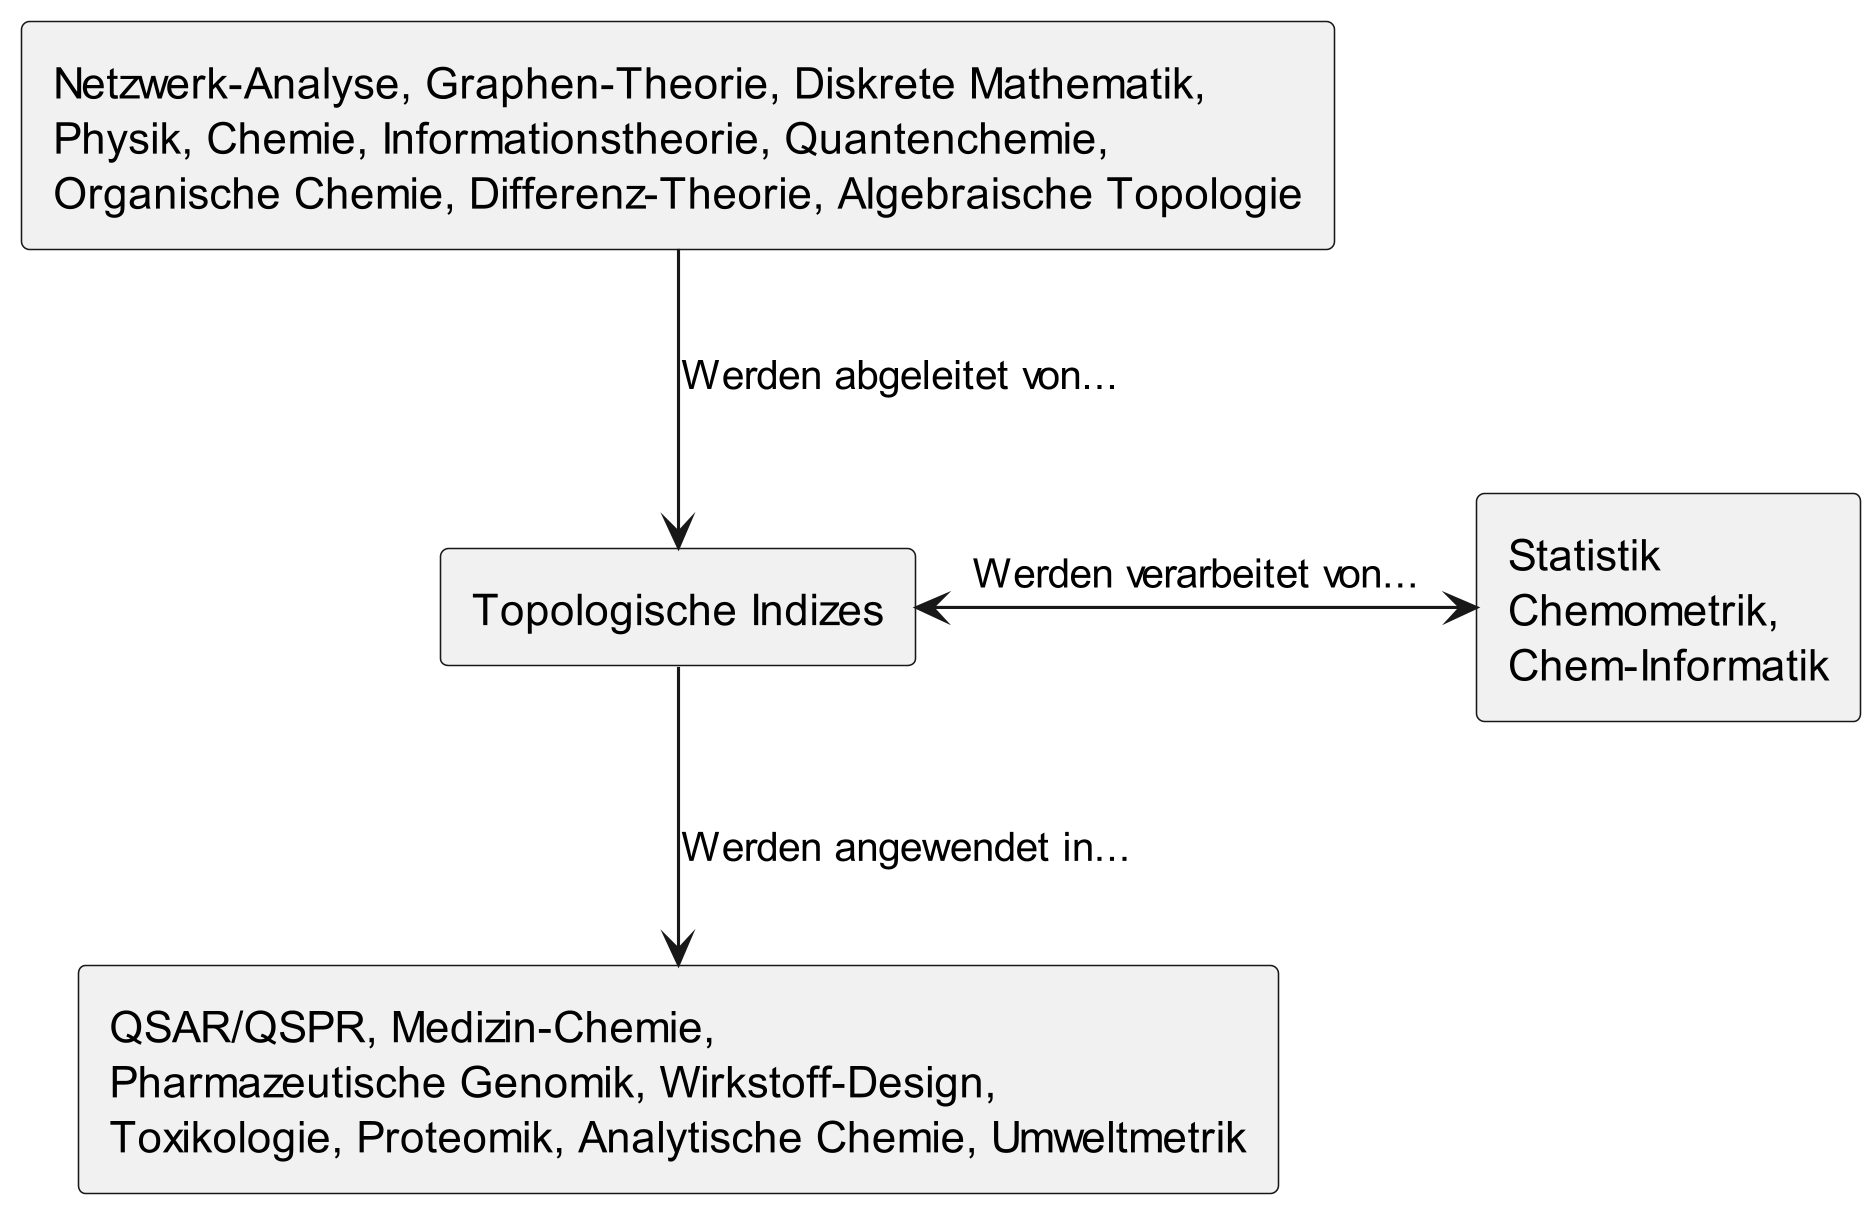
\includegraphics[width=0.9\textwidth]{images/10_introduction/overview_molecule_descriptor.png}
    \caption{Übersicht zur Anordnung des Themengebietes, übersetzt aus Todeschini und Consonni \cite{todeschini_handbook_2000}}
    \label{fig:overview_indices}
\end{figure}

Eine der Hauptanwendungen der Graphentheorie ist die Darstellung und Analyse von Netzwerken.
Beispielsweise kann ein soziales Netzwerk als Graph dargestellt werden, mit Menschen als Knoten und den Beziehungen zwischen ihnen (Freundschaften, familiäre Bindungen etc.) als Kanten.
Die Analyse der Struktur des Netzwerks kann Aufschluss darüber geben, wie sich Informationen im Netzwerk verbreiten und welche Faktoren die Veränderung des Netzwerks beeinflussen können \cite[p.~440ff.]{watts_collective_1998}.

Die Graphentheorie wird auch dazu verwendet, Probleme in der Informatik und den Ingenieurwissenschaften zu lösen.
Sie kann etwa genutzt werden, um den kürzesten Weg zwischen zwei Punkten in einem Verkehrsnetz zu finden \cite[p.~269]{dijkstra_note_1959} oder um Aufgaben in einem Computersystem zu planen \cite[p.~9]{garey_computers_1990}.
In der Biologie kann die Graphentheorie eingesetzt werden, um die Wechselwirkungen zwischen Genen oder Proteinen in einer Zelle zu untersuchen \cite[p.~3]{albert_diameter_1999} und in der Soziologie, um die Struktur sozialer Netzwerke und deren Kommunikationsmuster zu analysieren \cite[p.~1ff.]{barnes_graph_1969}.

\section{Was ist ein Graph?}

Formell wird ein Graph als $G = (V, E)$ definiert, wobei $V$ die Menge der Knoten und $E$ die Menge der Kanten ist.
Knoten können als Punkte oder Kreise dargestellt werden und Kanten als Linien, die zwei Knoten verbinden \cite[p.~45]{barabasi_network_2016}.

Ein Graph kann \textbf{\textit{ungerichtet}} oder \textbf{\textit{gerichtet}} sein. Bei einem ungerichteten Graphen können die Kanten in beide Richtungen durchlaufen werden.
Bei einem gerichteten Graphen können die Kanten nur in eine Richtung durchlaufen werden.
Eine Kante kann auch \textbf{\textit{gewichtet}} oder \textbf{\textit{ungewichtet}} sein.
Gewichtete Kanten haben einen numerischen Wert, der als Kosten, Länge oder ähnliches interpretiert werden kann \cite[p.~46]{barabasi_network_2016}.

Auf Abbildung \ref{fig:general_graphs} folgt ein Beispiel für einen gerichteten, ungerichtet und gewichteten Graphen.

\begin{figure}[H]
    \centering
    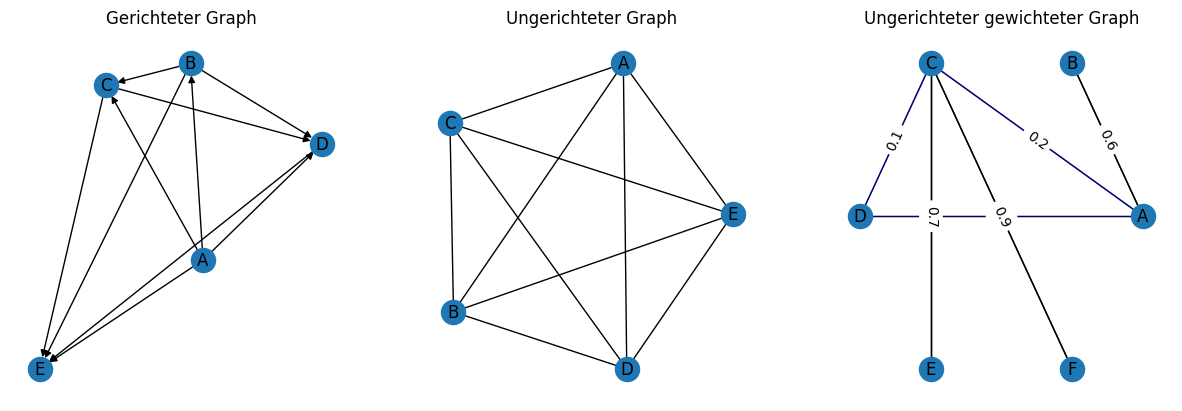
\includegraphics[width=0.9\textwidth]{images/10_introduction/graph_intro.png}
    \caption{Darstellung der verschiedenen Graphen}
    \label{fig:general_graphs}
\end{figure}

Ein Graph kann \textbf{\textit{zusammenhängend}} oder \textbf{\textit{unzusammenhängend}} sein.
Ein zusammenhängender Graph besteht aus einer einzigen zusammenhängenden Komponente, d. h. es gibt einen Pfad von jedem Knoten zu jedem anderen Knoten.
Ein unzusammenhängender Graph besteht aus mehreren Komponenten, die nicht miteinander verbunden sind.

Die \textbf{\textit{Ordnung}} eines Graphen ist die Anzahl der Knoten, die in ihm enthalten sind.
Die Grösse eines Graphen ist die Anzahl der Kanten, die in ihm enthalten sind.
Ein Graph mit $n$ Knoten kann höchstens $\frac{n(n-1)}{2}$ Kanten enthalten, wenn es sich um einen ungerichteten Graphen handelt \cite[p.~48]{barabasi_network_2016}.
Wenn es sich um einen gerichteten Graphen handelt, kann es höchstens $n(n-1)$ Kanten enthalten.

Ein wichtiger Begriff in der Graphentheorie ist der \textbf{\textit{Grad}} eines Knotens, der die Anzahl der Kanten beschreibt, die mit diesem Knoten verbunden sind. Im Falle eines ungerichteten Graphen ist der Grad eines Knotens einfach die Anzahl seiner Nachbarn. Im Falle eines gerichteten Graphen unterscheidet man zwischen dem Eingangsgrad, der Anzahl der Kanten, die auf den Knoten zeigen, und dem Ausgangsgrad, der Anzahl der Kanten, die vom Knoten wegführen. Der Grad eines Knotens kann dazu verwendet werden, die Verbindungsstärke zwischen den Knoten zu beschreiben und somit eine Aussage über die Struktur des Graphen zu treffen \cite[p.~48]{barabasi_network_2016} \cite[p.~14]{harary_graph_1994}.

Eine Möglichkeit, die Verbindungen zwischen den Knoten eines Graphen darzustellen, ist die Verwendung von \textbf{\textit{Adjazenzmatrizen}}. Eine Adjazenzmatrix ist eine quadratische Matrix, die die Verbindungen zwischen den Knoten des Graphen darstellt. Die Einträge der Matrix geben an, ob es eine Verbindung zwischen zwei Knoten gibt oder nicht. Im Falle eines ungerichteten Graphen ist die Adjazenzmatrix symmetrisch. Im Falle eines gerichteten Graphen ist die Adjazenzmatrix nicht symmetrisch. Die Verwendung von Adjazenzmatrizen kann helfen, die Struktur des Graphen zu verstehen und somit Aussagen über seine Eigenschaften und Funktionen zu treffen \cite[p.~51]{barabasi_network_2016} \cite[p.~151]{harary_graph_1994}.

Als Beispiel betrachten wir einen ungerichteten Graphen mit 4 Knoten, der wie folgt dargestellt werden kann:

\[
    A =
    \begin{bmatrix}
        0 & 1 & 1 & 0 \\
        1 & 0 & 1 & 0 \\
        1 & 1 & 0 & 1 \\
        0 & 0 & 1 & 0
    \end{bmatrix}
\]

In diesem Fall ist die Adjazenzmatrix symmetrisch, da der Graph ungerichtet ist. Die Einträge der Matrix geben an, ob es eine Verbindung zwischen zwei Knoten gibt oder nicht. Es gibt so etwa eine Verbindung zwischen Knoten 1 und Knoten 2, da der Eintrag $a_{1,2} = 1$ ist. Es gibt jedoch keine Verbindung zwischen Knoten 1 und Knoten 4, da der Eintrag $a_{1,4} = 0$ ist. Die Verwendung der Adjazenzmatrix kann helfen, die Struktur des Graphen zu visualisieren und Aussagen über seine Eigenschaften zu treffen.

Ein weiterer wichtiger Begriff in der Graphentheorie ist der \textbf{\textit{durchschnittliche Grad}} des Graphen, der angibt, wie viele Kanten jeder Knoten im Durchschnitt hat \cite[p.~48]{barabasi_network_2016}. Für einen ungerichteten Graphen mit $n$ Knoten und $m$ Kanten wird der durchschnittliche Grad $k$ wie folgt definiert:

$$k = \frac{2m}{n}$$

Für gerichtete Graphen unterscheidet man zwischen dem durchschnittlichen Eingangsgrad und dem durchschnittlichen Ausgangsgrad. Der durchschnittliche Grad gibt eine Aussage über die allgemeine Verbindungsstärke im Graphen und kann bei der Identifikation von Clusterstrukturen oder dem Vergleich von Graphen helfen \cite[p.~48]{barabasi_network_2016}.

Ein weiteres wichtiges Konzept in der Graphentheorie ist die \textbf{\textit{Gradverteilung}}. Die Gradverteilung beschreibt, wie viele Knoten in einem Graphen einen bestimmten Grad haben.

$$ P(k) := \frac{\delta_k}{N}$$

Wobei $|V| := N$ und $ \delta_k $ die Anzahl der Knoten mit Grad $k$ ist \cite[p.~311]{emmert-streib_mathematical_2020}.

Eine häufige Gradverteilung ist die Poisson-Verteilung, die für viele zufällige Graphen gilt. Eine andere häufige Gradverteilung ist die Potenzgesetz-Verteilung, die für viele reale Netzwerke gilt, wie in sozialen Netzwerken oder in der Biologie. Die Potenzgesetz-Verteilung ist charakterisiert durch einen hohen Anteil von Knoten mit niedrigem Grad und einem kleinen Anteil von Knoten mit hohem Grad, die als Hubs bezeichnet werden. Die Gradverteilung kann helfen, die Struktur eines Graphen zu verstehen und somit Aussagen über die Funktionsweise des Graphen zu treffen \cite[p.~51]{barabasi_network_2016}.

Die Zentralitätsmasse beschreiben, welche Knoten im Graphen besonders wichtig sind \cite[p.~313]{emmert-streib_mathematical_2020}.
Die Zentralität eines Knotens kann auf verschiedene Arten gemessen werden.
Eine Möglichkeit ist die \textbf{\textit{Degree-Zentralität}}, die angibt, wie viele Kanten mit einem Knoten verbunden sind.
Ein Knoten mit hoher Degree-Zentralität hat viele Nachbarn und ist somit wichtiger als ein Knoten mit niedriger Degree-Zentralität.
Die Degree-Zentralität $C_D(v)$ eines Knotens $v$ in einem ungerichteten Graphen $G=(V,E)$ wird wie folgt definiert:

$$C_D(v) = k_v$$

wobei $k_v$ die Anzahl der Nachbarn von $v$ ist \cite[p.~314]{emmert-streib_mathematical_2020}.

Ein weiteres Mass für die Zentralität ist die \textbf{\textit{Betweenness-Zentralität}}, die angibt, wie oft ein Knoten auf dem kürzesten Pfad zwischen anderen Knoten liegt.
Ein Knoten mit hoher Betweenness-Zentralität spielt eine wichtige Rolle bei der Vermittlung von Information zwischen anderen Knoten.
Die Betweenness-Zentralität $C_B(v)$ eines Knotens $v$ in einem ungerichteten Graphen $G=(V,E)$ wird wie folgt definiert:

$$C_B(v_k) = \sum_{v_i, v_j \in V, v_i \ne v_j} \frac{\sigma_{v_i v_j}(v_k)}{\sigma_{v_i v_j}}$$

wobei $\sigma_{v_i v_j}$ die Anzahl der kürzesten Pfade von $v_i$ nach $v_j$ ist und $\sigma_{v_i v_j}(v_k)$ die Anzahl der kürzesten Pfade von $v_i$ nach $v_j$ durch $v_k$ ist \cite[p.~314]{emmert-streib_mathematical_2020}.


\section{Netzwerkklassen} \label{sec:graph_classes}

Netzwerkklassen sind eine Sammlung von Netzwerken, die bestimmte Eigenschaften teilen.
Diese Eigenschaften können z. B. die Zahl der Knoten, die Anzahl Kanten oder die topologischen Indizes sein.
Brandstädt et al. und später Bang-Jensen et al. sowie Emmert-Streib et al. fassen populäre Graph-Modelle respektive Graphenklassen in verschiedenen Werken zusammen \cite{brandstadt_graph_1999,bang-jensen_basic_2018,emmert-streib_mathematical_2020}.
In den nachfolgenden Abschnitten folgen die bedeutendsten Netzwerkklassen nach \cite{emmert-streib_mathematical_2020}.
Sie bilden die Grundlage für die Weiterarbeit in der Thesis und werden vor allem in der Datenaufbereitung und den Experimenten verwendet.

Nachfolgend werden die Eigenschaften der unterschiedlichen Netzwerkklassen \enquote{Random}, \enquote{Small World} und \enquote{Scale-free} miteinander verglichen.
Dabei werden die Struktur, die Verteilung der existierenden Grade und die Adjazenzmatrix visualisiert und beschrieben.
Zur Einführung sind reguläre, zufällige und Small-World-Graphen auf Abbildung \ref{fig:random_scale_small} visualisiert.

\begin{figure}[H]
    \centering
    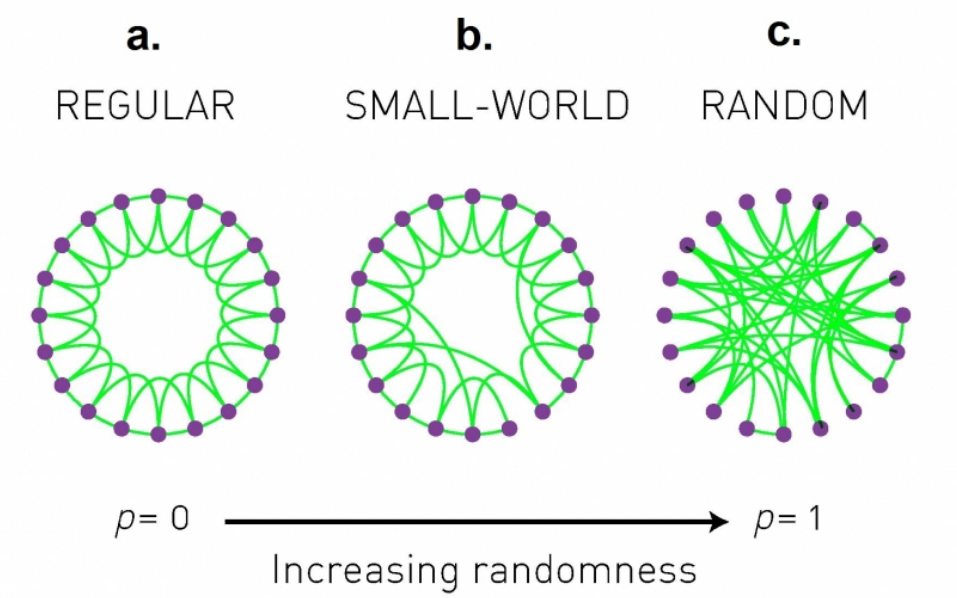
\includegraphics[width=7cm]{images/20_material_methods/barabasi_zusammenhang_smallworld_random.png}
    \caption{Eigenschaften der unterschiedlichen Netzwerkklassen (Quelle: Barabási \cite[p.~97]{barabasi_network_2016})}
    \label{fig:random_scale_small}
\end{figure}

\newpage
\subsection{Random}

Ein Zufallsgraph (engl. random graph) ist ein Graph, der zufällig gemäss einer Wahrscheinlichkeitsverteilung über die Menge aller möglichen Graphen generiert wird.
Das Studium von Zufallsgraphen ist ein Zweig der Graphentheorie und der probabilistischen Kombinatorik.

Ein gängiges Modell zum Erzeugen eines Zufallsgraphen ist das Erdős-Rényi-Modell, bei dem jede mögliche Kante unabhängig mit einer festen Wahrscheinlichkeit $p$ aufgenommen wird \cite[p.~205 ff]{grimmett_random_nodate}.
Dieses Modell ist umfassend untersucht und weist besonders interessante Eigenschaften auf wie den Phasenübergang, der bei der kritischen Wahrscheinlichkeit $p = 1/n$ auftritt, wobei $n$ die Anzahl der Scheitelpunkte im Graphen ist \cite[p.~152]{bollobas_random_2001}.

Des Weiteren ist das bevorzugte Bindungsmodell (engl. preferential attachment) zu nennen, das einen Zufallsgraphen erzeugt, indem es mit einer kleinen Anzahl von Scheitelpunkten beginnt und nacheinander neue Scheitelpunkte hinzufügt, von denen jeder mit einer bestimmten Wahrscheinlichkeit proportional mit vorhandenen Scheitelpunkten verbunden ist \cite[p.~2f]{albert_diameter_1999}.
Dieses Modell wird häufig verwendet, um das Wachstum von sozialen Netzwerken oder des World Wide Web (WWW) zu modellieren.
Es gibt zahlreiche andere Modelle zum Generieren von Zufallsgraphen, jedes hat seine einzigartigen Eigenschaften. Einige Beispiele sind das Small-World, das Watts-Strogatz und das k-reguläre Modell \cite[p.~398f.]{newman_networks_2010}.

Das Studium von Zufallsgraphen hat zu einem tieferen Verständnis der Struktur und Eigenschaften realer Graphen sowie zur Entwicklung effizienter Algorithmen zum Generieren und Analysieren grosser Graphen geführt.
Auf Abbildung \ref{fig:random_graphs} sind drei Zufallsgraphen ersichtlich; gewisse Knoten besitzen einen Grad $k = 0$, was bedeutet, dass sie isoliert sind und keine Kanten haben \cite[p.~85]{barabasi_network_2016}:

\begin{figure}[H]
    \centering
    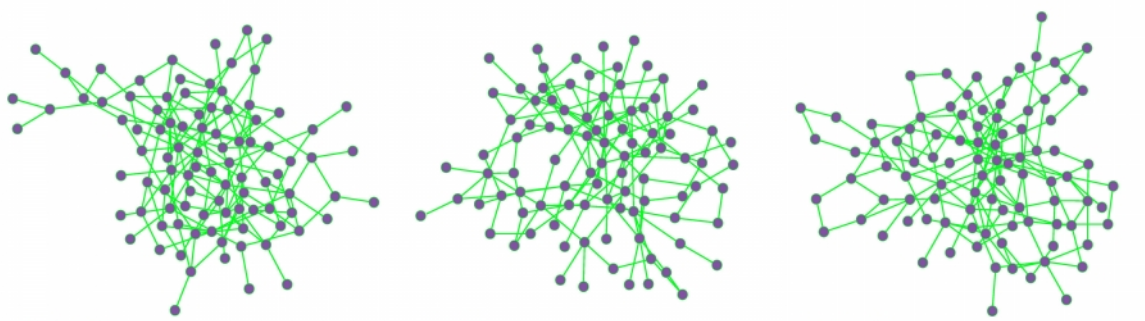
\includegraphics[width=11cm]{images/20_material_methods/random_graphs.png}
    \caption{Drei Random-Graphen mit $\protect p = 0.03$ und $\protect N = 100 $ (Quelle: Barabási. \cite[p.~84]{barabasi_network_2016})}
    \label{fig:random_graphs}
\end{figure}

\newpage
\subsection{Small World}

Ein Small-World-Graph ist eine Art komplexes Netzwerk, das sowohl eine hohe Clusterbildung als auch eine kurze durchschnittliche Pfadlänge aufweist.
Das Konzept der Small-World-Graphen ist erstmals in den 1960er-Jahren von Stanley Milgram durch das \enquote{Six Degrees of Separation}-Experiment eingeführt worden.
Er hat gezeigt, dass zwei beliebige Menschen auf der Erde durchschnittlich über sechs Bekanntschaften verbunden sind  \cite[p.~62]{travers_experimental_1969}

Ende der 1990er-Jahre haben Duncan J. Watts und Steven H. Strogatz das Konzept der Small-World-Graphen weiterentwickelt und den Begriff \enquote{Small-World Networks} eingeführt \cite[p.~440]{watts_collective_1998}.
Sie haben damit gezeigt, dass Small-World-Netzwerke durch eine hohe Clusterbildung gekennzeichnet sind, was bedeutet, dass Knoten in der Regel mit anderen Knoten zusammenhängen, die wiederum eng mit diesen verbunden sind, genauer gesagt durch eine kurze durchschnittliche Pfadlänge.
Dies heisst, dass es unkompliziert ist, jeden Knoten im Netzwerk durch eine vergleichsweise kleine Anzahl von Schritten zu erreichen.

Watts und Strogatz (1998) definieren in ihrem Modell zum Aufbau von Small-World Networks $n$ Knoten, wobei jeder Knoten mit $m$ nächsten Nachbarn verbunden ist.
Dies wird als reguläres Gitter bezeichnet (siehe Abbildung \ref{fig:small_world}), wobei $n = 10$ und $m = 4$ ist  \cite{gayen_small_2020}.
\begin{figure}[H]
    \centering
    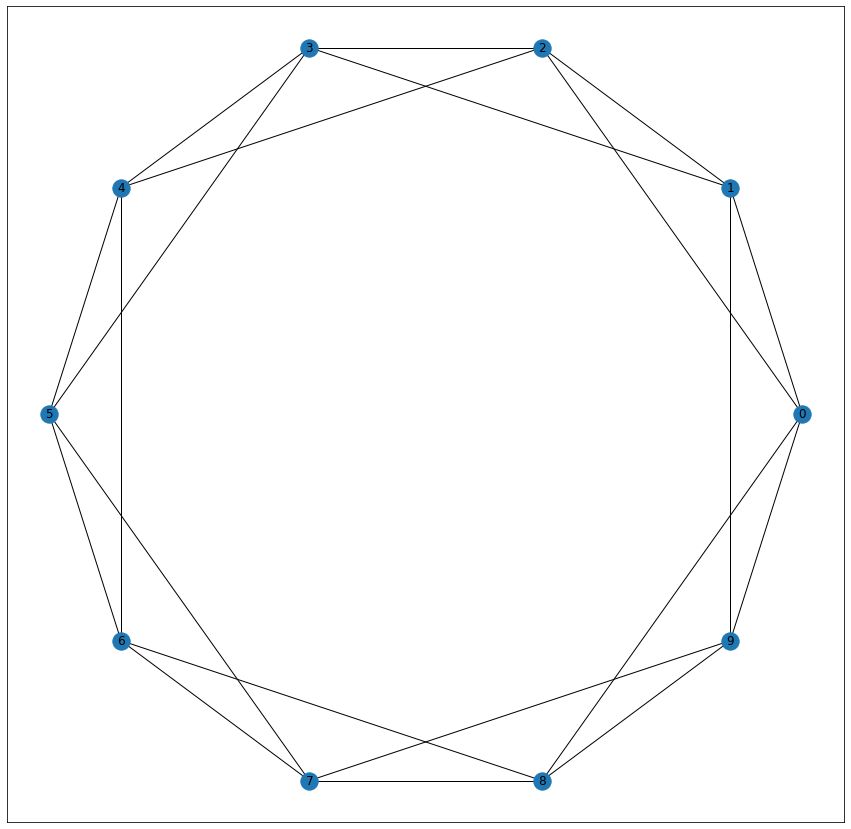
\includegraphics[width=3cm]{images/20_material_methods/small_world_lattice.png}
    \caption{Regular Lattice Graph (Quelle: Gayen \cite{gayen_small_2020})}
    \label{fig:small_world}
\end{figure}
Bei Betrachtung einer jeden Kante $(u, v)$ wird mit der Wahrscheinlichkeit $p$ zufällig ein Knoten $w$ ausgewählt und die Kante $(u, v)$ so verbunden, dass sie zu $(u, w)$ wird.
Für $p = 0$ behält es seine Struktur und hat einen hohen durchschnittlichen Abstand und eine hohe Clusterbildung.
Für $p = 1$ wird ein Zufallsnetzwerk mit kleiner durchschnittlicher Distanz und geringer Clusterbildung gebildet \ref{fig:small_world_lattice_n10}, wobei $n = 10$, $m = 4$ und $p = 1$ ist.
Für einen Zwischenwert von $p$ erhält man ein ideales Small-World Network mit geringer durchschnittlicher Entfernung und hoher Clusterbildung \cite{gayen_small_2020}.
\begin{figure}[H]
    \centering
    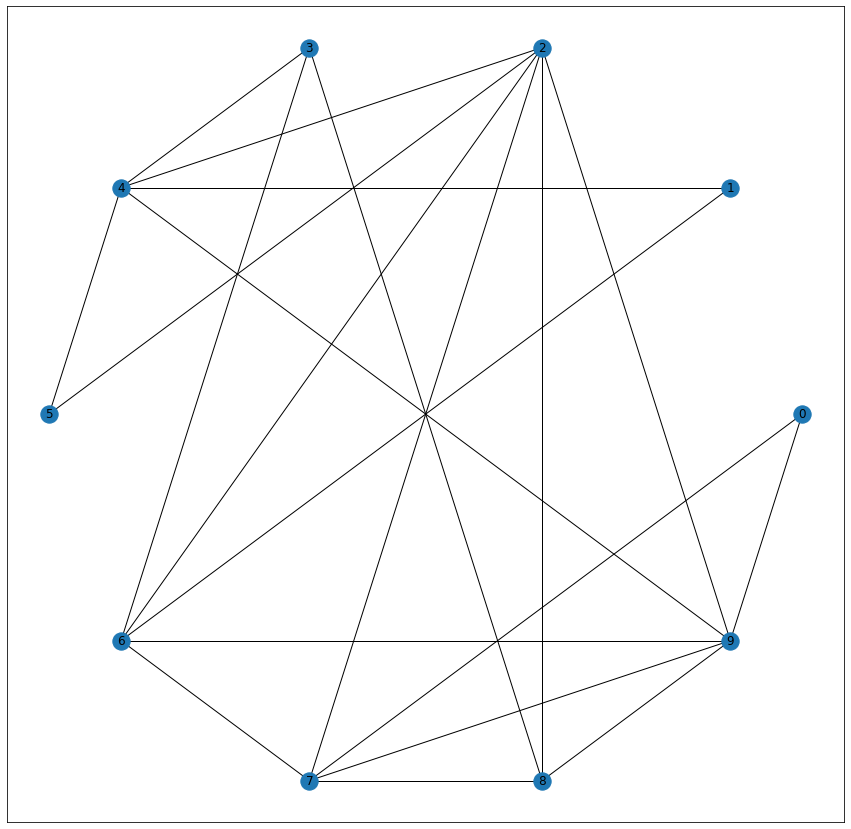
\includegraphics[width=3cm]{images/20_material_methods/small_world_lattice_n10.png}
    \caption{Regular Lattice Graph mit $n = 10, m = 4$ und $p = 1 $ (Quelle: Gayen \cite{gayen_small_2020})}
    \label{fig:small_world_lattice_n10}
\end{figure}
Es hat sich herausgestellt, dass Small-World-Graphen in Systemen der realen Welt weitverbreitet sind, darunter soziale Netzwerke, Transportnetzwerke und das Internet \cite[p.~4]{barabasi_emergence_1999}.
Sie werden auch in verschiedenen Bereichen wie Physik, Biologie und Informatik untersucht, da sie bedeutende Auswirkungen auf die Verbreitung von Informationen und die Robustheit von Netzwerken haben \cite[p.~2]{newman_structure_2003}.

\subsection{Scale-free}

In der Anfangsphase des Web, in den 1990er-Jahren, wurde davon ausgegangen, dass dieses die Eigenschaften eines zufälligen Netzwerks hat, des Netzwerktyps, der von Erdős–Rényi (1960) mathematisch charakterisiert wurde und in dem die Wahrscheinlichkeit für die Verbindung zweier Knoten als Konstante angegeben ist.
In einem derartigen Netzwerk folgt die Gradverteilung der Poisson-Form \cite{barabasi_network_2016}.

Albert et al. (1999, S. 1) haben gezeigt, dass das WWW nicht diese zufällige Netzwerkstruktur hat \cite{albert_diameter_1999}.
Tatsächlich ist die Gradverteilung ein Potenzgesetz, bei dem die Wahrscheinlichkeit, dass ein Knoten den Grad $k$ hat, proportional zu $k-\lambda$ ist, wobei $\lambda$ etwa $2$ ist.
Ein solches Netzwerk hat andere Eigenschaften, als ein zufälliges Netzwerk, da ein Potenzgesetz weniger stark abfällt als eine Poisson-Kurve.
Anstatt dass praktisch alle Knoten mehr oder weniger den gleichen Grad haben, sind einige wenige Knoten äusserst stark verbunden und die überwiegende Mehrheit hat einen geringeren Grad als der Durchschnitt \cite{barabasi_network_2016}.

\subsection{Bäume}

Ein Baum (engl. Tree) ist ein gerichteter Graph, der keine Schleifen und Kreise enthält.
Das bedeutet, dass jeder Knoten genau einen Vorgänger hat und dass es einen eindeutigen Pfad von jedem Knoten zum Wurzelknoten gibt \cite{cayley_analytical_1881}.

Die Verwendung von Bäumen ist eine gängige Methode zur Simulation von Hierarchien und Untersuchung von Struktureigenschaften in komplexen Netzwerken.
Zum Beispiel kann ein Baum Graph verwendet werden, um die Verteilung von Informationsflüssen in einem Netzwerk zu untersuchen oder um die Effekte von Strukturänderungen auf die Effizienz von Netzwerken zu bewerten \cite{brandstadt_graph_1999}.

Ein weiterer Vorteil von Baum Graphen ist, dass sie einfach zu generieren sind und wenig Rechenaufwand erfordern.
Daher sind sie für Anwendungen zweckmässig, bei denen schnelle und einfache Simulationen erforderlich sind, insbesondere bei der Analyse von grossen Netzwerken. Zudem können Baum Graphen auch verwendet werden, um statistische Eigenschaften komplexer Netzwerke zu schätzen, etwa die Verteilung von Knotengrössen oder die Anzahl der Verbindungen zwischen Knoten.

Insgesamt bieten Baum Graphen eine geeignete Methode zur Analyse von Hierarchien und Strukturen in komplexen Netzwerken.
Sie benötigen wenig Rechenaufwand und bieten relevante Informationen über die Eigenschaften von Netzwerken.
Daher sind sie ein wesentlicher Bestandteil der Netzwerktheorie und werden oft in der Praxis verwendet \cite{cayley_analytical_1881,emmert-streib_mathematical_2020}.

\begin{figure}[H]
    \centering
    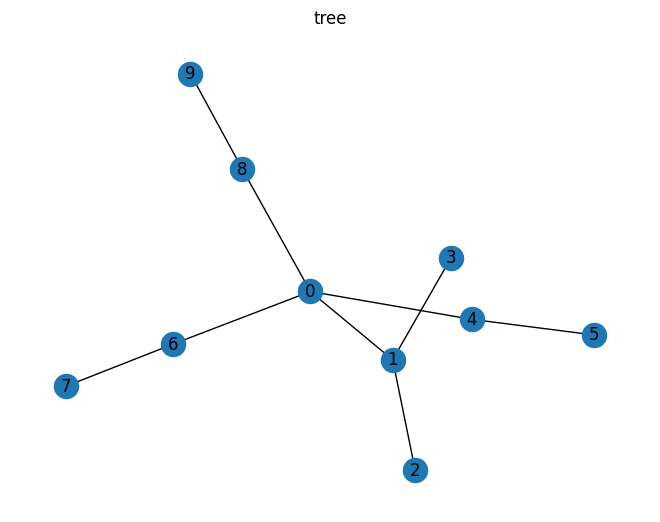
\includegraphics[width=6cm]{images/20_material_methods/tree.png}
    \caption{Baum Graph}
    \label{fig:tree-graph}
\end{figure}

\subsubsection{Sterne}

Sterngraphen sind eine Klasse von ungerichteten Graphen und eine Unterklasse von Bäumen, bei denen ein Knoten (zentraler Knoten) direkt mit allen anderen Knoten (Peripherie-Knoten) verbunden ist. 
Ein Sterngraph mit $n$ Knoten kann als $S_n$ dargestellt werden. 
Der zentrale Knoten in einem Sterngraphen hat $n-1$ Kanten, während jeder Peripherie-Knoten nur eine Kante hat.

Die Formel für die Anzahl der Kanten eines Sterngraphen lautet:
\begin{equation}
    \text{E}(S_n) = n-1
\end{equation}
Sterngraphen haben folgende Eigenschaften:
\begin{enumerate}
    \item Sie besitzen $n$ Knoten und $n-1$ Kanten.
    \item Sie haben keine Schleifen.
    \item Ihr Durchmesser ist $\min{2, n}$.
    \item Sie sind zusammenhängend.
\end{enumerate}

Sie sind einfach zu konstruieren und zu analysieren und werden oft verwendet, um Probleme in verschiedenen Bereichen zu lösen.

\begin{figure}[H]
    \centering
    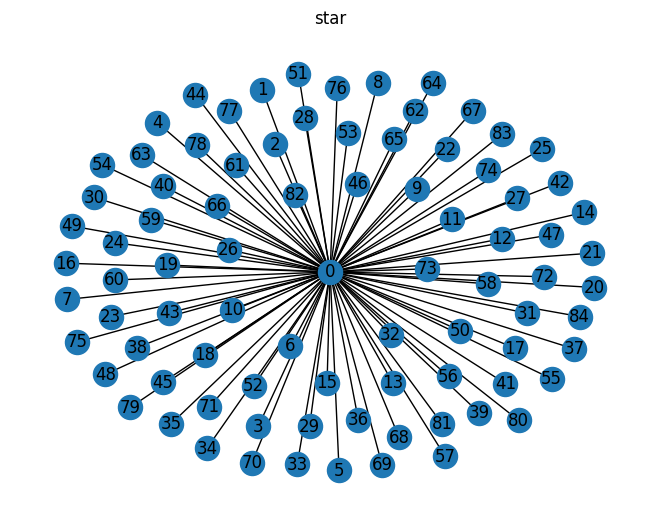
\includegraphics[width=6cm]{images/20_material_methods/star.png}
    \caption{Sterngraph}
    \label{fig:star-graph}
\end{figure}

\subsection{Vollständig} \label{sec:complete}

Vollständige Graphen sind eine bedeutsame Klasse von Graphen in der Mathematik, die eine vollständige Verbindung aller Knoten innerhalb des Graphen darstellen.
Bei einem vollständigen Graphen mit $n$ Knoten ist jeder Knoten mit jedem anderen direkt verbunden.
Ein vollständiger Graph mit $n$ Knoten kann als $G(n)$ dargestellt werden.

Die Formel für die Anzahl der Kanten eines vollständigen Graphen lautet \cite[p.~53]{barabasi_network_2016}:
\begin{equation}
    \text{E}(G(n)) = \frac{n(n-1)}{2}
\end{equation}

Ein Complete Graph ist ein besonderer Fall des k-regulären Graphen, bei dem jeder Knoten eine gleichmässige Anzahl von Kanten hat.
Er ist der maximale k-reguläre Graph für $k = n-1$ \cite{bang-jensen_basic_2018}.

\begin{figure}[H]
    \centering
    \includesvg[width=4cm]{images/20_material_methods/k5-graph.svg}
    \caption{K5-Graph}
    \label{fig:k5-graph}
\end{figure}

\subsection{Path}

Path Graphs, auch bekannt als Pfadgraphen, sind eine einfache Klasse von Graphen, die eine gerichtete Kette von Knoten darstellen.
Ein Path Graph mit $n$ Knoten kann als $P_n$ dargestellt werden.
Jeder Knoten in einem Pfadgraphen hat genau eine eingehende und eine ausgehende Kante, ausser dem ersten Knoten, der nur eine ausgehende, und dem letzten Knoten, der nur eine eingehende Kante hat.

Die Formel für die Anzahl der Kanten eines Path Graph lautet:
\begin{equation}
    \text{E}(P_n) = n-1
\end{equation}

Path Graphs finden häufig Anwendung in der Mathematik, insbesondere bei der Untersuchung von Problemen in der Graphtheorie und Netzwerktheorie \cite{bender_lists_2010}. 
Zum Beispiel können Path Graphs verwendet werden, um den kürzesten Pfad in einem Netzwerk zu untersuchen, und sie können auch als Bausteine für die Konstruktion von grösseren Graphen verwendet werden.

\begin{figure}[H]
    \centering
    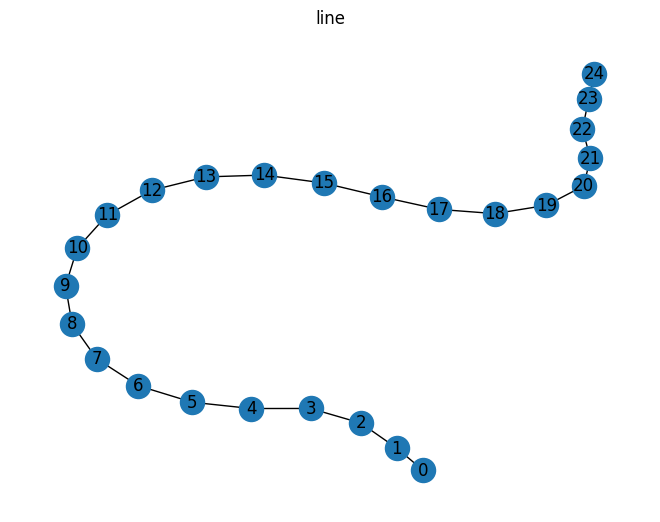
\includegraphics[width=6cm]{images/20_material_methods/path.png}
    \caption{Path oder Line Graph}
    \label{fig:path-graph}
\end{figure}


\newpage
\section{Topologische Indizes} \label{sec:topologische_indizes}

Topologische Indizes sind mathematische Masse, die die topologische Struktur eines Graphen charakterisieren.
Sie können genutzt werden, um die Konnektivität oder Komplexität eines Netzwerks zu beschreiben, und sie haben zahlreiche Anwendungen in einer Vielzahl von Bereichen:
In der Chemie dienen topologische Indizes dazu, die Eigenschaften chemischer Verbindungen wie Siede-, Schmelzpunkte und Löslichkeit vorherzusagen.
Sie können auch verwendet werden, um die strukturellen und funktionellen Eigenschaften von Biomolekülen wie Proteinen und Nukleinsäuren zu untersuchen.
In der Biologie kann mithilfe von topologischen Indizes, um die Protein-Ligand-Bindungsaffinität vorhergesagt werden, was für das Arzneimitteldesign bedeutsam ist.
Topologische Indizes können auch zur Untersuchung der Struktur und Funktion biologischer Netzwerke eingesetzt werden, etwa Protein-Protein-Interaktionsnetzwerke und metabolische Netzwerke \cite[p.~199ff]{balaban_topological_1983}.
In sozialen Netzwerken können topologische Indizes verwendet werden, um die Struktur von Netzwerken zu analysieren und zu verstehen, wie sich Informationen durch diese verbreiten.

Der topologische Index ist ein numerischer Wert oder eine Sequenz für eine bestimmte diskutierte Struktur, die tatsächlich die physikalischen, chemischen und biologischen Eigenschaften eines Graphen abbildet \cite{manzoor_entropy_2020}.
Einige Indizes spiegeln die Grösse des Moleküls wider, z. B. der Kohlenstoffzahlindex, andere, z. B. der Balaban-Zentralindex, charakterisieren die Form \cite[p.~1]{rouvray_modeling_1987}.
\begin{theorem}[Topologischer Index]
    \label{thm:topologischer_index}%
    Ein topologischer Index ist eine numerische Invariante eines Graphen \cite[p.~235]{plavsic_harary_1993}.

    Topologische Indizes sind Zahlen, welche Graphen durch konstitutionelle Formeln aus mathematischen Operationen als numerische Werte repräsentieren. \cite[p.~16]{devillers_topological_2000}, \cite[p.~23]{devillers_topological_2000}.
\end{theorem}

\newpage
\subsection{Anwendung von topologischen Indizes}

Eine der Hauptanwendungen topologischer Indizes ist die Untersuchung der Eigenschaften chemischer Verbindungen, um diese basierend auf ihren strukturellen und funktionellen Eigenschaften zu klassifizieren. Topologische Indizes werden auch zugrunde gelegt, um die Struktur und Funktion von Biomolekülen wie Proteinen und Nukleinsäuren zu untersuchen \cite[p.~1015]{gonzalez-diaz_medicinal_2007}.
Topologische Indizes dienen auch dazu, wesentliche Einflussfaktoren zu identifizieren oder vorherzusagen, wie sich das Netzwerk im Laufe der Zeit verändern könnte \cite[p.~400]{watts_collective_1998}.

Topologische Indizes werden auch angewendet, um Probleme in anderen Bereichen wie Informatik, Ingenieurwesen und Wirtschaftswissenschaften zu lösen. So werden sie beispielsweise eingesetzt, um den kürzesten Weg zwischen zwei Punkten in einem Transportnetzwerk zu finden \cite{dijkstra_note_1959} und um die Ressourcenallokation in einer Lieferkette zu optimieren \cite{bazaraa_nonlinear_2013}.
Insgesamt liegt der Nutzen topologischer Indizes in ihrer Fähigkeit, ein quantitatives Mass für die topologische Struktur eines Graphen bereitzustellen, das zur Untersuchung der Eigenschaften komplexer Systeme und zur Lösung von Problemen in einer Vielzahl von Bereichen verwendet werden kann.

Topologische Indizes werden u. a. von Chemikern als Werkzeug zur Beschreibung chemischer Phänomene genutzt.
Die topologischen Indizes charakterisieren dabei sowohl die Grösse als auch die Form chemischer Spezies und spiegeln die Menge an Verzweigungen in Molekülen signifikant wider.
Chemiker sind somit in der Lage, das chemische Verhalten einer breiten Palette chemischer Substanzen in allen drei thermodynamischen Zuständen graphenbasiert genau zu modellieren \cite[p.~1]{rouvray_modeling_1987}.

Eine ihrer Eigenschaften, die als Einzigartigkeit oder Unterscheidungskraft bezeichnet wird, ist in der mathematischen Chemie und im strukturorientierten Arzneimitteldesign im Kontext der quantitativen Charakterisierung der Struktur von Molekülen ausführlich untersucht worden.
Im Allgemeinen erhält ein Index das Attribut degeneriert, wenn er für mehr als einen Graphen denselben Wert besitzt \cite[p.~1]{dehmer_information_2012}.

Weitere Wissenschaftler haben magnitudenbasierte Informationsindizes vorgeschlagen, um die Trennschärfe anderer klassischer topologischer Index für Alkanbäume und Isomere zu verbessern.
Alkanbäume sind zusammenhängende und azyklische Graphen, in denen der Grad eines Knotens höchstens 4 ist.
Zudem wird die Trennschärfe von informationstheoretischen Massen basierend auf Distanzen für chemische Graphen unterschieden, die einen Ring enthalten.
So ist die Einzigartigkeit verschiedener informationstheoretischer und nicht informationstheoretischer Massnahmen gegeben, indem polyzyklische Strukturen verwendet werden.
Als Ergebnis erweisen sich der Balaban-J-Index, die Summe der lokalen Vertex-Entropien und die magnitudenbasierten Informationsindizes als einzigartig, für diese Klasse von Graphen \cite[p.~1]{dehmer_information_2012}.

Neben empirischen Eigenschaften von Informationsmassen für Graphen – etwa das Bestimmen von Korrelationen zwischen den Massen – bestehen auch mathematische Probleme, z. B. der Nachweis verschiedener Ober- und Untergrenzen von Massnahmen.
Die Korrelationsfähigkeit zwischen zwei Graphmassen bezieht sich im Allgemeinen auf das Problem, ob sie strukturelle Informationen ähnlich erfassen.
Ausserdem wird die Klasse der Graphen-Entropiemasse, die durch Verwendung bestimmter Informationsfunktionale auf Grundlage der metrischen Eigenschaften von Graphen (z. B. der Nachbarschaft von Atomen) erhalten werden, verwendet, um Probleme in QSAR und QSPR zu lösen.
Insbesondere Dehmer et al. (2012) klassifizieren die sog. Mutagenität von Molekülen unter Verwendung dieser Massnahmen und unter Nutzung überwachter Lerntechniken \cite[p.~2]{dehmer_information_2012}.

Insgesamt werden in dieser Studie die Grenzen topologischer Indizes und Restriktionen bei deren Anwendung im grossen Massstab deutlich. Ein topologischer Index kann für eine bestimmte Graphenklasse eindeutig sein, aber er schlägt fehl, wenn das Mass auf eine andere Klasse angewendet wird \cite[p.~9]{dehmer_information_2012}.

Topologische Indizes \(TI(G)\) haben folgenden Anforderungen zu erfüllen:

\begin{lemma}[Topologische Indizes und Isomorphie]
    \label{thm:index_isomorphism}%
    Wenn \(G_1 \simeq G_2 \) (isomorph) sind, dann gilt \(TI(G_1) = TI(G_2)\).
    Im Umkehrschluss gilt bei \(TI(G_1) = TI(G_2)\), \( G_1 \simeq G_2\) nicht, da Indizes bei nicht isomorphen Graphen auch denselben Wert ergeben können.
\end{lemma}

Dieses Lemma wird in den zwei nachstehenden Beispielen verdeutlicht.

\begin{figure}[H]
    \begin{subfigure}{.4\textwidth}
        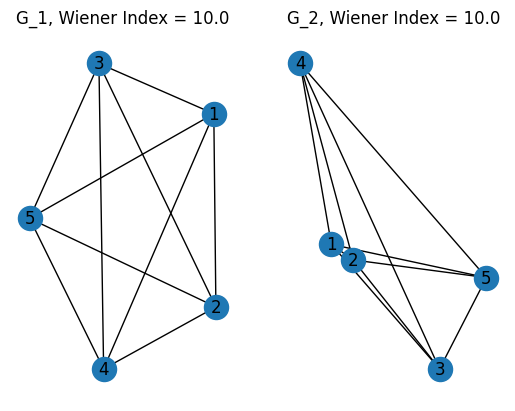
\includegraphics[width=\textwidth]{images/20_material_methods/lemma_2_proof_1.png}
        \label{fig:lemma_proof_1}
    \end{subfigure}%
    \hfill
    \vline
    \hfill
    \begin{subfigure}{.4\textwidth}
        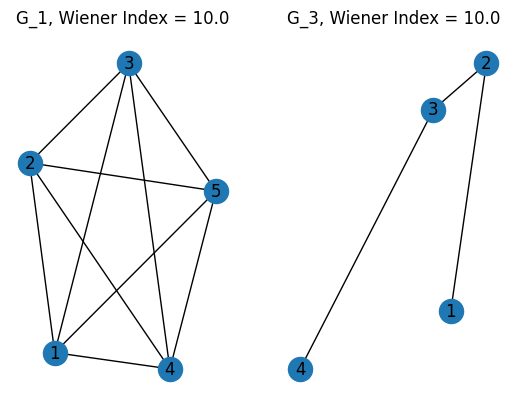
\includegraphics[width=\textwidth]{images/20_material_methods/lemma_2_proof_2.png}
        \label{fig:lemma_proof_2}
    \end{subfigure}
    \caption{Nachweis von Lemma \ref{thm:index_isomorphism}. G\_1 und G\_2 links, sind isomorphe Graphen. G\_1 und G\_3 in der rechten Abbildung sind nicht isomorphe Graphen, aber haben denselben Wiener Index.}
\end{figure}

Die topologischen Indizes können nach Balaban in verschiedene Kategorien eingeteilt werden \cite{balaban_1983_2014}.
Dabei spricht er von den folgenden Klassen: gradbasiert (Adjazenzmatrix), distanzbasiert (Distanz-Matrix), zentrische Indizes und informationstheoriebasiert.

\subsection{Gradbasiert}

Sei $\mathcal{G}$ ein molekularer Graph. Zwei Knoten von $\mathcal{G}$, die durch eine Kante verbunden sind, heissen \enquote{benachbart}.
Sind zwei Knoten $u$ und $v$ benachbart, besteht die Beziehung $u ~ v$.
Die Anzahl der Knoten von $\mathcal{G}$, die an einen gegebenen Knoten $v$ angrenzen, ist der \enquote{Grad} dieses Knotens und wird mit $dv(\mathcal{G})$ bezeichnet – wenn die Eindeutigkeit gegeben ist, mit $dv$.
Das Konzept des Grades in der Graphentheorie ist eng verwandt mit dem Konzept der Valenz in der Chemie \cite[p.~351]{gutman_degree-based_2013}.

\begin{figure}[H]
    \centering
    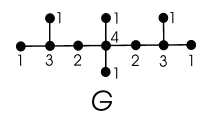
\includegraphics[width=0.3\textwidth]{images/20_material_methods/degree_graph.png}
    \caption{Graph $\mathcal{G}$ mit den Knotengeraden (Quelle: \cite[p.~351]{gutman_degree-based_2013})}
    \label{fig:degree_graph}
\end{figure}

Somit hat $\mathcal{G}$ sechs Knoten vom Grad $1$ (sogenannte \enquote{hängende} Knoten, die Methylgruppen darstellen) und zwei Knoten vom Grad 2 sowie zwei vom Grad 3 und einen Knoten vom Grad 4. Aus chemischen Gründen können die molekularen Graphen von Kohlenwasserstoffen keine Knoten besitzen, deren Grad grösser als 4 ist \cite[p.~351]{gutman_degree-based_2013}.

\subsubsection{Randić-Index}

Der Randić-Index und der Generalized Randić-Index sind Masse für die Struktur von Molekülen in der Chemie.
Der Randić-Index wurde von Milan Randić entwickelt und ist ein Mass für die \enquote{Heterogenität} oder die Unterschiedlichkeit der Atome in einem Molekül \cite{li_survey_2008}.

Er wird wie folgt berechnet:
\begin{equation}
    R = \sum_{uv \in E(G)}\frac{1}{\sqrt{d_u d_v}}
\end{equation}
Hierbei ist $d(i)$ die Anzahl der Nachbarn des Atoms $i$ und die Summe läuft über alle Atome des Moleküls.

Im Jahr 1998 haben Bollobás und Erdős den generalized Randić Index definiert, bei welchem auch die Anzahl der Bindungen zwischen den Atomen berücksichtigt wird \cite{li_survey_2008}.

Er wird folgendermassen berechnet:
\begin{equation}
    R_{\alpha}(G) = \sum_{uv \in E}{d(u) d(v)}^{\alpha}
\end{equation}
Im Allgemeinen wird der Generalized Randić-Index verwendet, wenn mehr Informationen über die Struktur eines Moleküls erlangt werden sollen, insbesondere über die Anzahl und Art der Bindungen zwischen den Atomen.
Der Randić Index hingegen ermöglicht nur Informationen über die Anzahl der Nachbarn eines Atoms und ist daher weniger detailliert.

Des Weiteren ist der $R_{\alpha}$ mit einem $\alpha = +1$ unter dem Namen \textit{Second Zagreb Index} definiert \cite{li_survey_2008}.

\subsubsection{Zagreb-Index}

Der erste Zagreb-Index wurde 1972 von Gutman und Trinajstic definiert \cite{xu_zagreb_2011}.
Er ist gleich der Summe der quadrierten Nachbarschaftsgrade aller Knoten.
\begin{equation}
    M_1(G) = \sum_{u \in V (G)} deg(v)^2
\end{equation}
Der zweite Zagreb-Index wird folgendermassen definiert:
\begin{equation}
    M_2(G) = \sum_{uv \in E (G)} deg(u) deg(v)
\end{equation}
Er ist die Summe der Produkte der Knotengrade von benachbarten Knoten \cite{das_zagreb_2015}.

\subsubsection{Harmonischer Index}

Der harmonische Index ist eine Variante des Randić-Index \cite[p.~562]{zhong_harmonic_2012}.
Er ist als die Summe der Gewichte aller Kanten von $uv$ von $G$ definiert, wobei $d(u)$ den Grad eines Knotens $u$ in $G$ abbildet.
Für einen Graphen $G$ lautet wird er wie berechnet \cite[p.~562]{zhong_harmonic_2012}:
\begin{equation}
    H(G) = \sum_{uv \in E (G)} \frac{2}{d(u) + d(v)}
\end{equation}
Die Berechnung des harmonischen Index kann aufwendig sein, insbesondere für grosse Graphen, aber es gibt Algorithmen und Techniken, um ihn effizient zu berechnen. 
Der harmonische Index hat auch interessante mathematische Eigenschaften und ist ein aktives Forschungsgebiet in der Graphentheorie \cite{li_harmonic_2014}.

\subsubsection{Atom-Bond Connectivity Index}

Dieser Index beschreibt die Verbindungen zwischen den Atomen einer Verbindung und berechnet den Index auf der Basis der Anzahl der Bindungen, die jedes Atom hat.
Die Verwendung von gradbasierten Metriken zur Charakterisierung von Verbindungen ist ein bedeutender Aspekt in der chemischen Informatik, und der Atom-Bond-Connectivity (ABC) Index ist eine gängige Methode zur Bewertung der Atomkonnektivität in Verbindungen \cite{estrada_atom-bond_1998}.

Die Formel zur Berechnung des ABC-Index lautet:
\begin{equation}
    ABC = \sum_{uv \in E(G)} \sqrt{\frac{d_u + d_v - 2} {d_u \times d_v}}
\end{equation}
Hierbei sind $d_u$ und $d_v$ die Grade der Knoten $u$ und $v$.

\subsection{Distanzbasiert}

\subsubsection{Wiener-Index}

Der Wiener-Index ist der erste topologische Index, der von Harold Wiener, einem Chemiker, eingeführt wurde \cite{fath-tabar_hyper-wiener_2011}.
Ein fundamentaler, distanzbasierter Index ist der Wiener-Index. Er ist als Summe der Abstände zwischen allen ungeordneten Scheitelpunktpaaren des Graphen definiert und heute aufgrund des breiten Anwendungsspektrums weitgehend verbreitet.
Insbesondere ist er einer der am häufigsten verwendeten topologischen Indizes in der mathematischen Chemie.
Angesichts dessen korreliert es stark mit vielen physikalischen und chemischen Eigenschaften molekularer Verbindungen, deren Eigenschaften nicht nur von ihrer chemischen Formel, sondern auch von ihrer molekularen Struktur abhängen \cite[p.~2]{cavaleri_group_2021}.
Es werden die Summen aller Abstände (kürzeste Wege) von jedem Knoten zu jedem anderen Knoten in die Berechnung einbezogen.
Der Wiener-Index ist definiert durch \cite[p.~17]{wiener_structural_1947}:
\begin{equation}
    W = \frac{1}{2}\sum^N_{i,j}d_{ij}
\end{equation}

\subsubsection{Hosoya-Index} \label{sec:hosoya_index}

Der Hosoya-Index, auch molekularer topologischer Index genannt, ist ein mathematisches Mass für die topologische Komplexität eines Moleküls.
Er ist definiert als die Summe der Quadrate des Grades jedes Scheitelpunkts im Molekulargraphen, wobei der Grad eines Scheitelpunkts die Anzahl der damit verbundenen Kanten ist.
Der Hosoya-Index korreliert nachweislich mit verschiedenen physikalischen und chemischen Eigenschaften von Molekülen wie Siedepunkt und Löslichkeit \cite[p.~397ff]{hosoya_topological_1972}.

Eine der frühesten wissenschaftlichen Arbeiten zum Hosoya-Index ist 1981 von F. Hosoya und Y. Tanaka in der Zeitschrift Chemical Physics Letters veröffentlicht worden.
In diesem Artikel stellen die Autoren das Konzept des Hosoya-Index vor und demonstrieren sein Potenzial als Mass für die molekulare Komplexität.
Seit seiner Einführung ist der Hosoya-Index auf dem Gebiet der chemischen und biochemischen Forschung weitverbreitet und Gegenstand zahlreicher wissenschaftlicher Arbeiten und Übersichtsartikel \cite[p.~397ff]{hosoya_topological_1972}.

Er wird folgendermassen berechnet \cite[p.~182]{hosoya_topological_1972}:
\begin{equation}
    Z = \sum_{k = 0}^{\lfloor N / 2 \rfloor} p(G, k)
\end{equation}
Dabei ist $ p(G, k) $ die Anzahl Möglichkeiten, in welcher $ k $ Knoten von $ G $ gewählt werden können, so dass keine zwei Knoten benachbart sind.
Das in den Gauss-Klammern stehende $ N / 2 $ ist die kleinste natürliche Zahl innerhalb $ N / 2 $.
Den grössten Hosoya-Index eines Graphen mit $ n $ Knoten erhält man von einem kompletten Graphen \ref{sec:complete}.

\subsubsection{Szeged-Index}

Der Szeged-Index ist ein Mass für den Informationsgehalt eines Graphen und wird verwendet, um die Komplexität oder Struktur des Graphen zu bewerten.
Er ist von Ivàn Gutman 1994 eingeführt worden und generalisiert das Konzept des Wiener-Index \cite{gutman_szeged_1998}.

Er lässt sich folgendermassen berechnen \cite[p.~2]{gutman_szeged_1998}:
\begin{equation}
    Sz(G) = \sum_{e \in E(G)} n_1(e | G)n_2 (e | G)
\end{equation}
Hier ist $ e $ eine Kante aus $ E $ im Graphen $ G $; $ e $ verbindet die Knoten $ u $ und $ v $, so wird auch $ e = uv $ oder $ e = vu $ geschrieben.
Für $ e = uv \in E(G) $ sei $ n_1(e | G) $ und $ n_2(e | G) $ die Anzahl Knoten von $G$, die näher zu Knoten $ u $ als Knoten $ v $ respektive für $n_2$ näher bei Knoten $ u $ als Knoten $ v $ sind \cite{gutman_szeged_1998}.

\subsection{Zentrische Indizes}

Die zentrischen Indizes wurden durch Balaban eingeführt und sind eine Gruppe von Indizes, die die zentrische Struktur eines Graphen beschreiben \cite{balaban_1983_2014}.
Sie verhalten sich ähnlich wie die Distanz-Indizes, da es bei der Suche nach dem zentralen Knoten auf die Distanz zwischen den Knoten ankommt.
Gemäss dem Jordanschen Zentrumssatzes ist der zentrische Knoten derjenige, der die geringste Summe der Distanzen zu allen anderen Knoten hat \cite[p.~32]{gross_graph_2018}. \\
Die Definition des Zentrums eines Graphens $ G $ ist eine Menge von Knoten $ V $, deren \textit{graph eccentricity} gleich dem Graph-Radius ist \cite[p.~35]{harary_graph_1994}.

\subsubsection{Balabans zentrischer Index B}

Der zentrische Index $B$ von Balaban wurde Entwickelt, um das Zentrum von Baumgraphen zu bestimmen \cite[p.~355]{balaban_chemical_1979}.
$ B $ wird ähnlich wie der erste Zagreb-Index aufgrund der quadratischen Formel definiert \cite[p.~355]{balaban_chemical_1979}.
\begin{equation}
    B = \sum_{i} \delta_i^2
\end{equation}

Dabei ist $ \delta_i $ die Anzahl Knoten, welche bei jedem Schritt $ i $ entfernt werden können, ohne dass der Graph zerfällt \cite[p.~355]{balaban_chemical_1979}.

\subsubsection{Estrada-Index}

Der Estrada-Index $ EE $ ist ein topologischer Index, welchen Estrada im Jahr 2005 eingeführt hat \cite{estrada_subgraph_2005}. 
Seinen Namen hat er jedoch erst 2007 von de la Peña \cite{de_la_pena_estimating_2007} erhalten. Er misst die Partizipation von allen Knoten in allen Teilgraphen eines Graphen \cite[p.~6]{estrada_subgraph_2005} und wird wie folgt berechnet \cite[p.~6]{estrada_subgraph_2005}:
\begin{equation}
    EE(G) = \sum_{i=1}^n e^{\lambda_i}
\end{equation}
Es ist $ G $ der Graph, $ n $ die Anzahl der Knoten und $ \lambda_i $ sind die Eigenwerte der Adjazenzmatrix $ A $.

\subsection{Informationstheoriebasiert}

Unter \enquote{Informationstheorie} wird ein Zweig der Mathematik verstanden, in dem die Quantifizierung und Analyse von Informationen thematisiert wird \cite[p.~82-83]{dehmer_information_2008}.
Informationstheoriebasierte Indizes stellen Masse dar, die Prinzipien der Informationstheorie verwenden, um den Informationsgehalt oder die Komplexität eines Systems quantitativ zu bewerten.
Ein Beispiel für einen auf der Informationstheorie basierenden Index ist die Entropie, die ein Mass für das Ausmass der Unsicherheit oder Zufälligkeit in einem System darstellt \cite[p.~767-768]{dehmer_information_2011}.
Entropie kann verwendet werden, um den Informationsgehalt einer Nachricht zu messen, indem bspw. das Ausmass der Unsicherheit quantifiziert und durch Erhalt der Nachricht reduziert wird \cite[p.~3]{iceland_multigroup_2004}.
Newman \cite[p.~2ff]{newman_structure_2003} diskutiert in diesem Kontext die Verwendung informationstheoretischer Indizes, einschliesslich der Entropie und gegenseitiger Informationen, um die Entwicklung von Informationen in komplexen Systemen zu untersuchen, die Zentralität von Knoten in Netzwerken zu quantifizieren sowie die Struktur und Funktion komplexer Netzwerke zu analysieren.

Balaban \cite[p.~16]{balaban_1983_2014} beschreibt zudem, dass laut einer Untersuchung die diversen informationstheoretischen Indizes eine tiefe diskriminierende Leistung aufweisen, was bedeutet, dass sie in der Lage sind, die Struktur eines Graphen zu unterscheiden, selbst wenn die Anzahl der Knoten und Kanten überaus gross ist. Eine Ausnahme ist der Balaban-J-Index.
Es ist später im Paper ein \emph{Super-Index} eingeführt worden, welcher ein Vektor ist, der aus den verschiedenen informationstheoretischen Indizes besteht \cite[p.~16]{balaban_1983_2014}. Dieser Super-Index besteht aus dem Informations-Orbit-Index $ I_{ORB}$, dem chromatischen Informationsindex $ I_{CHR} $, dem Graph-Distanz-basierten Informationsindex $ I^W_D $, dem Hosoya- und Randić-Informationsindex $ I_Z $ und $ I^E_X $ so wie dem orbitalen Informationsindex für Graphenverbindungen $ I_C $. \\
Im Rahmen dieser Arbeit wird jedoch nur der chromatische Informationsindex $ I_{CHR} $ untersucht.

\subsubsection{Chromatic Information Index}

Der Chromatic Information Index (CII) $ I_{CHR} $ ist ein Mass für den Informationsgehalt eines Graphen und wird verwendet, um die Komplexität oder Struktur des Graphen zu bewerten.
Er ist definiert als die Mindestanzahl von Farben, die erforderlich ist, um die Scheitelpunkte eines Diagramms richtig einzufärben, wobei Einschränkungen berücksichtigt werden,
die durch die Kanten zwischen den Scheitelpunkten vorgegeben werden. \\
Der CII ist ein nützliches Werkzeug zum Analysieren und Vergleichen der strukturellen Eigenschaften verschiedener Arten von Graphen und findet Anwendung in Bereichen wie Datenanalyse, Netzwerkwissenschaft und Informatik.
Er ist eng mit anderen Graphenfärbungsmassen wie der chromatischen Zahl, dem chromatischen Index und dem chromatischen Polynom verwandt \cite[p.~93ff]{bonchev_information_1985}.

Mowshowitz definiert den $ I_{CHR} $ als \textit{unique chromatic information content} (engl. für \enquote{einzigartiger chromatischer Informationsgehalt}) \cite[p.~13]{balaban_1983_2014}, welcher die chromatische Struktur eines Graphen repräsentiert \cite{mowshowitz_entropy_1968}.
\begin{equation}
    \hat{V} = \{ V_i \}^h_i=1(|V_i| = n_i(\hat{V}))
\end{equation}
Es ist $n$ die Anzahl der Knoten im Graphen $X$.
Es sei $\hat{V}$ die arbiträre chromatische Dekomposition von $X$, wo $h = \chi(X)$ gilt.
Dann sei $ I_{CHR}(X) $ der chromatische Informationsinhalt von $X$.
\begin{equation}
    I_{CHR}(X) = \min{V \{ -\sum_{i=1}{h}{\frac{n_i(V)}{n} \log \frac{n_i(V)}{n}} \} }
\end{equation}


\newpage
\section{Graphenklassifikation} \label{sec:classification_theory}

Die Graphenklassifikation ist eine Aufgabe, über welche Graphen einer oder mehreren Klassen zugewiesen werden.
Der Anfang der Graphenklassifikationstheorie liegt im Ansatz von Sobik. Er erläutert, wie die ersten Versuche zu einer Klassifikation stattgefunden haben und später, mit dem Einsatz von Machine Learning, eine effizientere Methode gefunden wurde.
Zum Schluss folgt die Methode, welche auch in der Erarbeitung der Resultate verwendet wird: der Einsatz von Graph Neural Networks.
Eine Übersicht über den historischen Verlauf der Graphenklassifizierung ist von Müller et al. in \cite{prokop_comparing_2013} festgehalten.

\subsection{Klassifikation auf Basis von Isomorphismus} \label{isomorphismus}

Bereits im Jahr 1974 hat Zelinka die Idee der Graphenklassifikation auf Basis von Isomorphismus eingeführt \cite{zelinka_certain_1975}.
Nachfolgend hat Sobik diese Methode für Graphen mit verschiedenen Knoten generalisiert \cite{sobik1}.

\paragraph{Graph-Isomorphie}
Eine Isomorphie zwischen zwei Objekten ist eine Bijektion zwischen ihren Mengen, bei der die Beziehungen erhalten bleiben. Der Isomorphismus ist eine Äquivalenzrelation auf der Menge aller Objekte \cite{mckay_practical_2014}.
Ein Graph $G$ ist isomorph zu einem Graphen $G'$, wenn es eine Abbildung $\phi: V(G) \rightarrow V(G')$ gibt, welche die Kanten von $G$ auf $G'$ abbildet.

$ G = [V, E, f, g, W_V, W_E] $ heisst (endlicher, gerichteter, interpretierbarer) \textbf{Graph} gdw. $V$ eine endliche Menge und $ E \subseteq V \times V $ ist, $ W_V $ und $ W_E $ endliche, nichtleere Mengen und $ f: V \rightarrow W_V $ und $ g: E \rightarrow W_E $ Funktionen von $V$ bzw. $E$ in $W_V$ bzw. $W_E$ sind \cite[p.~65]{sobik1}.

$ H = [V', E', f', g', W_V, W_E] $ heisst \textbf{Teilgraph} von $G$ gdw. $V' \subseteq V$ und $E' \subseteq E \cap (V' \times V') $ ist und $f'$ und $g'$ Einschränkungen von $f$ bzw. $g$ auf $V'$ bzw. $E'$ sind. Gilt $E' = E \cap (V' \times V')$, dann heisst $H$ \textbf{induzierter Untergraph} von $G$.
Dabei ist $V$ die Knotenmenge und $E$ die Kantenmenge des Graphen $G$, $W_V$ und $W_E$ sind die Mengen möglicher Knoten- bzw. Kanteninterpretationen und $f$ und $g$ die entsprechenden Markierungsfunktionen \cite[p.~65]{sobik1}.

Seien $G = [V, E, f, g, W_V, W_E] $ und $H = [V', E', f', g', W_V, W_E] $ Graphen. $G$ und $H$ heissen isomorph $(G \cong H)$ gdw. eine eineindeutige Abbildung $\varphi$ von $V \cup E$ auf $V' \cup E'$ existiert mit \cite[p.~65]{sobik1}:
\begin{align*}
    \varphi(v)          & \in V'                       & \forall v \in V                         \\
    \varphi(e)          & \in E'                       & \forall e \in E                         \\
    \varphi((v_1, v_2)) & = \varphi(v_1), \varphi(v_2) & \forall v_1,v_2 \in V, (v_1, v_2) \in E \\
    f(v)                & = f'(\varphi(v))             & \forall v \in V                         \\
    g(e)                & = g'(\varphi(e))             & \forall e \in E
\end{align*}

Nach der Definition der Graph-Isomorphie wendet sich Sobik dem Klassifizierungsproblem zu.
Er definiert die Menge der Graphen, die es erlauben, Graphen verschiedener Klassen zu unterscheiden als \enquote{klassifizierungsrelevant} \cite[p.~68]{sobik1}.

\subsection{Klassifizierung durch strukturelle Masse}

Harary legt dar, dass strukturelle Graphmasse, also topologische Indizes, für isomorphe Graphen gleich sind \cite{harary_graph_1994}.

Basak et al. verwenden strukturelle Graphmasse, um die strukturellen Ähnlichkeiten von verschiedenen Molekulargraphen festzustellen \cite{basak_topological_1987}.
Somit werden erste Ansätze zur Graphenklassifikation auf Basis von topologischen Indizes gelegt.

Eine Voraussetzung für die Klassifizierung durch topologische Indizes ist die Einzigartigkeit der einzelnen Indizes untereinander. Dehmer et al. haben bewiesen, dass ein informationstheoretischer Index basierend auf der Grad-Grad-Vereinigung eine grosse Unterscheidungskraft besitzt \cite{dehmer_information_2012}.

\subsection{Machine Learning – Support Vector Machine} \label{svm}

Nach 2000 sind diverse Werke erschienen, in denen die Graphenklassifikation mit Machine-Learning-Methoden gelöst worden sind. Es werden Support Vector Machines (SVM) eingesetzt, um Protein-Netze für die Krebsforschung zu klassifizieren \cite{brown_knowledge-based_2000,guyon_gene_2002}.

Müller et al. beschreiben den Einsatz von Graph-Kernels, welche in einer ersten Form von Kashima und Inokushi \cite{kashima_kernels_2002} 2002 vorgeschlagen wurden. Dabei bilden Random-Walks den Kernel eines Graphen.
Drei Jahre später hat Borgwardt den Graph-Kernel-Ansatz ausgebaut, indem er den Kernel auf Basis des shortest paths der Knoten aufgebaut hat \cite{borgwardt_shortest-path_2005}.

\subsection{Machine Learning – Neural Networks} \label{graph_neural_networks}

Graph-Transformer sind ein Graph Neural Network, welches die Eigenschaften des Graphen in einen Vektor transformiert.
Graph-Representation-Learning und Graph Neural Networks sind Themen, welche in den vergangenen Jahren stark an Bedeutung gewonnen haben \cite{zhang_end--end_2018,velickovic_deep_2018,chen_alchemy_2019,hamilton_graph_2020,ying_transformers_2021}.
Die Idee der Transformer ist 2017 in der Sprachverarbeitung entstanden \cite{vaswani_attention_2017} und im Jahr 2021 auf Graphen übertragen worden \cite{dwivedi_generalization_2021}.
Das Forschungsfeld der Graph-Transformer ist überaus aktuell und wird stetig weiterentwickelt.

Für die Aufgabe \enquote{Graphenklassifikation} gibt es diverse Benchmarking-Datensätze \cite{huggingface_papers_2017,hu_open_2021}.
Die besten Resultate in diesem Segment erreicht der Graph-Transfoert U2GNN \cite{nguyen_universal_2022}.

Jeder Graph $G$ wird durch ${\mathcal{G} = (\mathcal{V}, \mathcal{E}, \{  \mathbf{{h}_{v}}^{(0)} \}_{ {v} \in {\mathcal{V}} } )}$ repräsentiert.

Dabei ist $ \mathcal{V} $ ein Set von Knoten, $ \mathcal{E} $ ein Set von Kanten und $ \mathbf{{h}_{v}}^{(0)} \in \mathbb{R}^d $ ein Vektor, welcher die Eigenschaften des Knotens $v$ repräsentiert \cite{nguyen_universal_2022}.

Als Training werden ein Set $ M $ von Graphen $ \{\mathcal{G}_m \}_{m=1}^M $ und ihre zugehörigen Labels $ \{y_m\}_{m=1}^M \subseteq \mathcal{Y} $ verwendet.

Die Aufgabe der Graphenklassifikation ist es, für jeden Graphen $ \mathcal{G}_m $ den Embedded Graph $ \mathbf{e}_{\mathcal{G}_m} $ zu bestimmen und sein dazugehöriges Label $ y_m $ vorauszusagen \cite{nguyen_universal_2022}.

\begin{figure}[H]
    \centering
    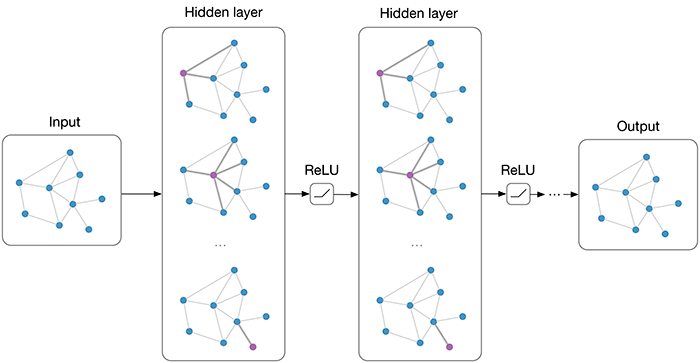
\includegraphics[width=0.8\textwidth]{images/20_material_methods/model.png}
    \caption{Modell für die Graphenklassifizierung (Quelle: \cite{kipf_semi-supervised_2017})}
    \label{fig:gcn_model}
\end{figure}

\newpage
\subsection{Unterschied von Graph-Embedding und Graph-Kernels}

Graph-Kernel-basierte Ansätze zersetzen einen Graphen in eine Menge von Subgraphen, Graphlets \cite{shervashidze_efficient_2009} oder Weisfeiler-Lehman-Kernels genannt \cite{shervashidze_weisfeiler-lehman_nodate}.
Diese Ansätze werden bisher verwendet, um die Ähnlichkeiten zwischen Graphen zu berechnen.
Beim Zersetzen von Graphen in Graph-Kernels geht es darum, möglichst viele Informationen auf ihre zentralen Merkmale zu reduzieren.
Diese Informationen werden dann in einem Vektor zusammengefasst und können mit anderen Vektoren verglichen werden.

Graph-Embedding ist ein Ansatz, welcher in den Graph Neural Networks verwendet wird. Der Ursprung geht auf William Hamilton und das Thema \enquote{Representation Learning} von Graphen zurück \cite{hamilton_inductive_2018}.
Die Aggregationsfunktion $ \phi $ ist ein Graph Neural Network, welches die Eigenschaften der Knoten in einen Vektor transformiert \cite{xu_how_2019}.
Mit der \textsc{ReadOut}-Funktion $ \rho $ werden die einzelnen Vektoren dann via Sum-Pooling zusammengefasst, um Graph-Embedding zu erhalten \cite{nguyen_universal_2022}.

\begin{figure}[H]
    \centering
    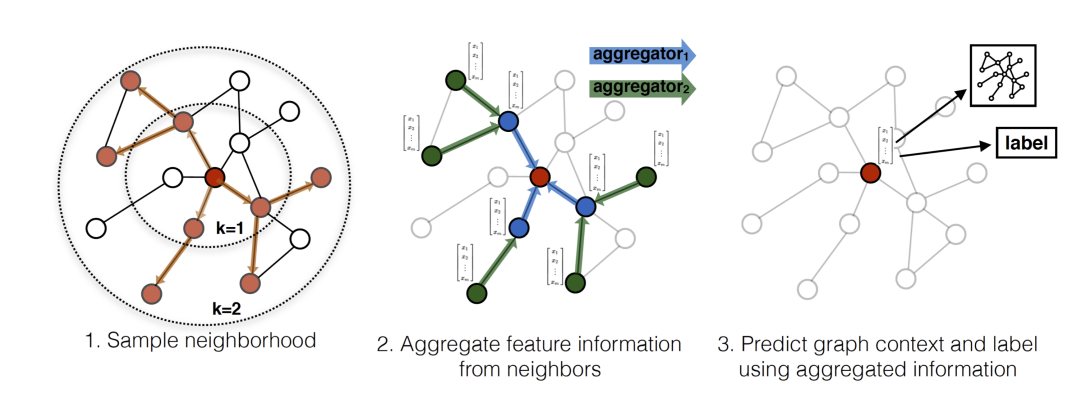
\includegraphics[width=9cm]{images/20_material_methods/graph_representation_learning.png}
    \caption{Sample- und Aggregation-Ansatz visualisiert (Quelle: Hamilton \cite{hamilton_inductive_2018})}
    \label{fig:graph_representation_learning}
\end{figure}


\newpage
\chapter{Eigene Resultate} \label{chap:results}

Die Theorie wird in Kapitel \ref{chap:results} verwendet, um die Resultate zu erläutern.
In diesen werden weitere topologische Indizes, die im theoretischen Teil nicht vorgestellt wurden, analysiert und verglichen.

Für aufschliessende Informationen zu allen aktuellen und bedeutsamen topologischen Indizes können bestehende Literaturwerke der Graphentheorie zurate gezogen werden \cite{dehmer_information_2012,ravi_computation_2022,amin_analysis_2022,sarkar_neighbourhood_2021}.
Der Werdegang der Graphenklassifikation wurde aufgearbeitet und das Thema Graph-Isomorphie erläutert.
Bei der Klassifikation wurden \textit{State-of-the-Art} Methoden und deren Hintergründe vorgestellt.
Als Nächstes folgen die verwendeten Daten für die Resultate sowie der Aufbau der Methodik.

Dieses Kapitel soll einen Überblick über die Resultate dieser Arbeit geben.
Es werden die visualisierten Resultate sowie die Ergebnisse der Tests zusammengefasst.
Die in der Einleitung \ref{chap:introduction} beschriebenen Hypothesen werden getestet und die erwarteten Resultate erarbeitet.

\newpage

\section{Erwartete Resultate}

Im Idealfall wird das Resultat eine quantitative Analyse verschiedener topologischer Indizes sein und einen Beitrag zur Usefulness von topologischen Indizes leisten.
Die quantitative Analyse umfasst eine explorative Datenanalyse der topologischen Indizes in verschiedenen Graph Klassen, eine statistische Analyse der Zusammenhänge zwischen den topologischen Indizes und den Graph-Klassen, so wie eine Machine Learning Analyse der Graph Klassen.

Mit der Analyse sollen die topologischen Indizes auf ihre Sinnhaftigkeit und Anwendbarkeit in verschiedenen Kontexten untersucht werden.
Als Resultat soll eine Auflistung respektive Rangfolge der sinnvollsten Messwerte für die eingegebenen Graphen und topologischen Indizes ausgegeben werden.
Der Algorithmus und die Formel zur Berechnung sollten möglichst einfach zugänglich und variabel sein. Der Code für die Berechnung soll Open Source sein.

Im Schlussteil der Arbeit sollen folgenden Resultate vorliegen:
\begin{itemize}
    \item eine sinnvolle Analyse und Auflistung der topologischen Messwerte,
    \item eine Analyse der Berechnung des Usefulness-Scores von topologischen Indizes in verschiedenen Netzwerkklassen,
    \item ein Python-Modul zur Berechnung des Usefulness-Scores und
    \item Vorschläge von topologischen Messwerten zur Struktur eines gelieferten Netzwerks.
\end{itemize}

Um diese Resultate zu erreichen, werden folgende Schritte durchgeführt:
\begin{enumerate}
    \item Datenaufbereitung,
    \item Durchführung von Experimenten,
    \item Entwicklung eines Systems, welches topologische Indizes sinnvoll vergleicht, sowie
    \item Implementierung der Systeme in Python.
\end{enumerate}

In der folgenden Übersicht ist dargestellt, wie die Erarbeitung der Resultate vonstattengeht:

\begin{figure}[H]
    \centering
    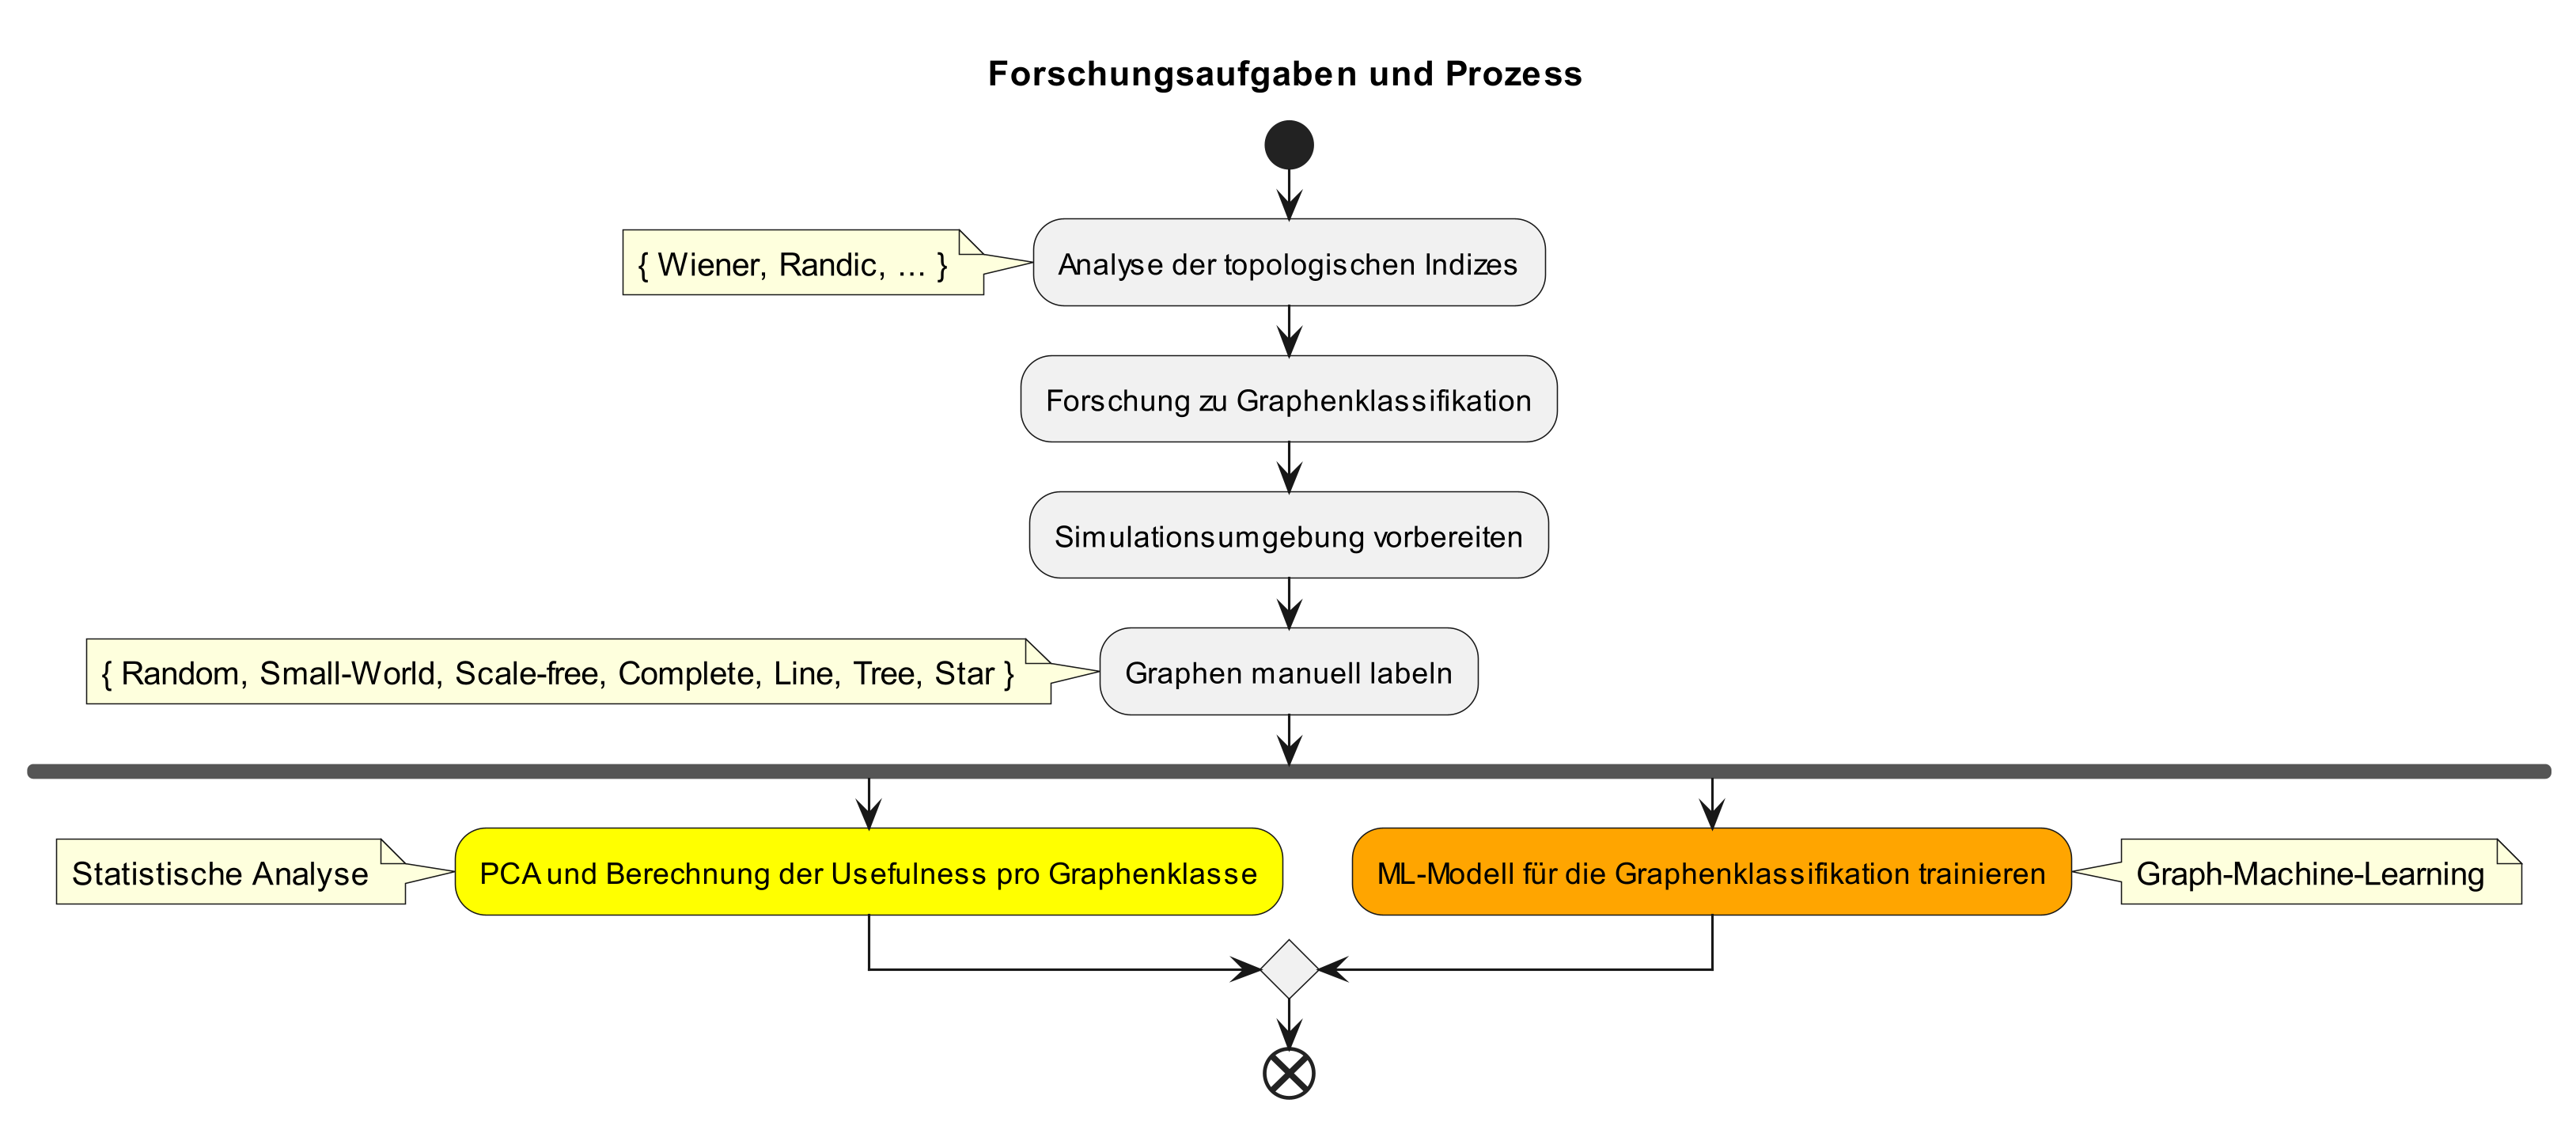
\includegraphics[width=1\textwidth]{images/30_results/activity_research.png}
    \caption{Erarbeitung der Resultate}
    \label{fig:results}
\end{figure}

Auf Abbildung \ref{fig:results} ist dargestellt, auf welchem Weg die Resultate erarbeitet werden. 
Gestartet wird mit der Analyse und Dokumentation der existierenden topologischen Indizes.
Der Studie zur Klassifikation von Graphen folgt das Beschaffen und Klassifizieren der Daten. 
Von da an ist die Arbeit in zwei parallele Arbeitsstränge geteilt. 
Mit einer statistischen Analyse werden die topologischen Indizes miteinander verglichen und daneben wird ein Machine-Learning-Modell entwickelt und trainiert, welches die Graphen klassifiziert. 
Die Resultate der beiden Arbeitsstränge werden zusammengeführt und die Hypothesen getestet.

\newpage

\section{Datenaufbereitung}

\subsection{Simulation}

In der Simulationsumgebung werden diverse Netzwerke mit verschiedenen topologischen Eigenschaften erzeugt und diese gemessen.
Zu Beginn werden verschiedene Netzwerke untersucht, darunter Nauty-Graphen, die aus dem Internet heruntergeladen wurden \cite{mckay_practical_2014}, sowie Netzwerke aus verschiedenen Anwendungsfällen wie biologische, soziale, chemische und Zitat-Netzwerke.

Um die Analyse zu formalisieren, liegt der Fokus der die Arbeit auf formelleren Klassen von Netzwerken.
Dadurch ergeben sich zwei Vorteile für die Analyse:
\begin{itemize}
    \item [+] Die Netzwerke können synthetisch erzeugt werden.
    \item [+] Die Klassen sind formal definiert und in der Literatur gut abgedeckt.
\end{itemize}

Es werden die in der Theorie zu den Netzwerkklassen \ref{sec:graph_classes} definierten Klassen verwendet.
Um Graphen zu generieren, müssen deren Parameter bzw. Eigenschaften dokumentiert werden.
Dadurch werden die Forschungsresultate aus dieser Arbeit reproduzierbar.
Im nächsten Abschnitt werden die genauen Netzstrukturen und ihre Eigenschaften beschrieben.

\newpage

\subsection{Netze und Klassen}

Es folgt das Fundament für die Daten der verwendeten Netzwerke.
Diese sind in verschiedene Klassen eingeteilt.

Die Daten werden eigenständig synthetisch mit Python generiert.
Es handelt sich bei allen Graphen um ungerichtete, zusammenhängende Graphen.

In dieser abgeschlossenen Liste sind die verwendeten Testdaten für die Netzwerkanalyse aufgeführt:

\begin{table}[H]
    \caption{\label{data-table}Alle Graphen, die für die Arbeit generiert wurden und deren Anzahl Knoten.}
    \begin{adjustbox}{minipage=\textwidth, center}
        \scriptsize
        \begin{tabularx}{\textwidth}{|l|X|X|c|}
            \hline
            \textbf{Name} & \textbf{Beschreibung}              & \textbf{Eigenschaften}                                                             & \textbf{Anzahl Graphen} \\
            \hline
            Random        & Random Erdős-Rényi-Graphen         & $ |V| = [5..205] $, \newline $ p = 0.3 $                                            & 1000                     \\
            \hline
            Small-World   & Watts-Strogatz Small-World-Graphen & $ |V| = [5..205] $, \newline $ k-neighbours = \frac{|V|}{2} $, \newline $ p = 0.3 $ & 1000                     \\
            \hline
            Scale-free    & Barabási-Albert-Graphen            & $ |V| = [2..202] $, \newline $ m = \frac{|V|}{2} $                                 & 200                      \\
            \hline
            Complete      & k-reguläre Graphen                & $ |V| = [2..202] $                                                                 & 200                      \\
            \hline
            Line          & Pfadgraphen                       & $ |V| = [2..202] $                                                                 & 200                      \\
            \hline
            Tree          & Bäume (+ Random-Trees)             & $ |V| = [2..11] | [2..202]$                                                          & 400                     \\
            \hline
            Star          & Sterngraphen                      & $ |V| = [2..202] $                                                                 & 200                      \\
            \hline
        \end{tabularx}
    \end{adjustbox}
\end{table}

Um ein besseres Bild der generierten Netze zu ermöglichen, folgt ein visualisiertes Beispiel pro Klasse:

\begin{figure}[H]
    \centering
    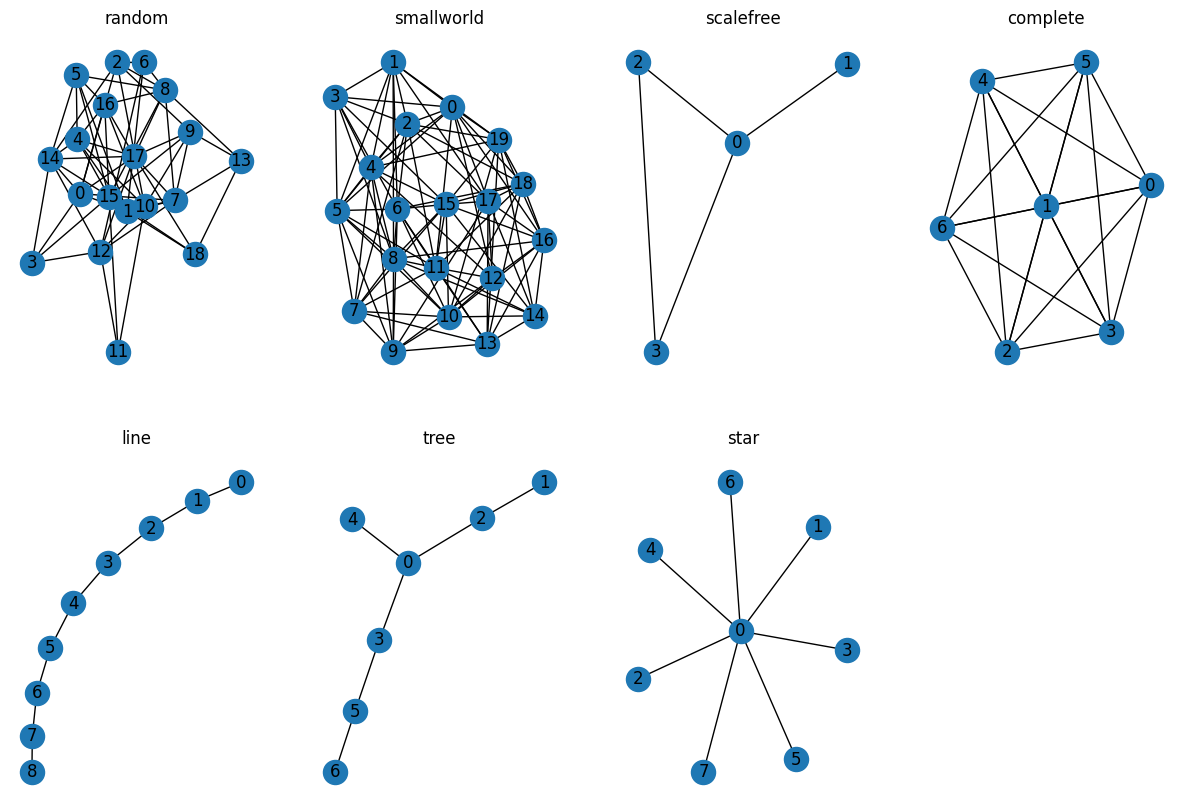
\includegraphics[width=0.6\textwidth]{images/42_data/example_graphs.png}
    \caption{Visualisierung von Graphen mit NetworkX und Matplotlib}
    \label{fig:example_graphs}
\end{figure}

Die Complete, Line-, Tree- und Star-Graphen unterscheiden sich schon bei der ersten Betrachtung stark.
Die Random-Graphen nach Erdős-Rényi und die Small-World-Graphen können auf den ersten Blick ähnlich aussehen, differieren jedoch in der topologischen Struktur, wie bereits in der Theorie erwähnt.

\subsection{Datenaufbereitung und Datenstruktur}

Die Graphen für die Arbeit werden mithilfe von Python und NetworkX erarbeitet \cite{hagberg_exploring_2008}.
Das erstellte Python-Dictionary mit den jeweiligen Graphen ist nachfolgend aufgeführt:

\begin{listing}[H]
    \begin{minted}
        [frame=lines,framesep=2mm,baselinestretch=1.2,bgcolor=LightGray,fontsize=\footnotesize,linenos]
        {python}    
dataset = {
    "random": [],
    "smallworld": [],
    "scalefree": [],
    "complete": [],
    "line": [],
    "tree": [],
    "star": [],
}
    \end{minted}
    \caption{Datenstruktur für die Testdaten}
\end{listing}

In einem nächsten Schritt werden die erstellten Graphen ihrer Klasse zugewiesen, was auch als \emph{Labeling} bezeichnet werden kann. Das Label der Graphen ist der Key des Dictionary.
Diese Labels werden für die spätere Klassifikationsaufgabe verwendet.

\newpage
\section{Vergleich der topologischen Indizes} \label{sec:correlation}

Die Graphen werden zunächst einer explorativen Datenanalyse unterzogen.
Dabei werden erste Zusammenhänge zwischen den topologischen Indizes und den Graphenklassen untersucht.

\subsection{Erste Erkenntnisse und Resultate}

Da es sich um einen mittelgrossen Datensatz handelt und die Knotenanzahl der Graphen generell nicht über 250 liegt, dauert die Berechnung der topologischen Indizes für das ganze Datenset circa 20–30 Minuten.
In der Theorie wurden die relevanten topologischen Indizes für die Analyse der Graphen beschrieben und ausgewählt.
Es gibt eine Vielzahl an Messwerten, die an dieser Stelle verwendet werden könnten.
Die Auswahl der topologischen Indizes ist eine subjektive Entscheidung, die auf der Erfahrung und dem Wissen des Autors basiert.
Später kann die Auswahl der topologischen Indizes erweitert werden, da der Code als parametrierbares, wiederverwendbares Modul entwickelt wird.
Es werden folgende topologische Indizes untersucht:

\begin{table}[H]
    \caption{Topologische Indizes unter Betrachtung}
    \begin{adjustbox}{minipage=\textwidth, center}
        \scriptsize
        \begin{tabularx}{\textwidth}{|l|X|c|}
            \hline
            \textbf{Name}                     & \textbf{Beschreibung}                                                                                                                                                                                                                                    & \textbf{Implementierung} \\
            \hline
            \textbf{Wiener-Index}             & Summe aller kürzesten Pfadlängen zwischen allen Paaren von Knoten in einem Graphen                                                                                                                                                                       & \textit{grinpy}          \\
            \hline
            \textbf{Randic-Index}             & Summe der Wurzel der Gradzahlen aller Knoten in einem Graphen                                                                                                                                                                                            & \textit{grinpy}          \\
            \hline
            \textbf{Generalized Randić-Index} & Erweiterung des Randić-Index, die nicht nur die Knotengrade berücksichtigt, sondern auch andere topologische Informationen wie die Distanz zwischen Knoten, um eine umfassendere Charakterisierung der topologischen Struktur von Graphen zu ermöglichen & \textit{grinpy}          \\
            \hline
            \textbf{Harmonic-Index}           & Harmonische Zentralität in Netzwerken, die als Summe der inversen harmonischen Mittelwerte aller kürzesten Pfadlängen zwischen jedem Knoten und allen anderen Knoten im Netzwerk definiert ist.                                                          & \textit{grinpy}          \\
            \hline
            \textbf{ABC-Index}                & Mass für die Konnektivität von Knoten in Graphen, definiert als Summe der Produkte aus den Gradzahlen der beteiligten Knoten und der Anzahl der Kanten zwischen ihnen                                                                                    & \textit{grinpy}          \\
            \hline
            \textbf{First Zagreb-Index}       & Summe der Quadrate der Gradzahlen aller Knoten in einem Graphen                                                                                                                                                                                          & \textit{grinpy}          \\
            \hline
            \textbf{Second Zagreb-Index}      & Summe der Produkte der Gradzahlen von Paaren benachbarter Knoten                                                                                                                                                                                         & \textit{grinpy}          \\
            \hline
            \textbf{Estrada-Index}            & Summe der Eigenwerte des Netzwerk-Adjazenzmatrix-Exponenten                                                                                                                                                                                              & \textit{networkx}        \\
            \hline
            \textbf{Hosoya-Z-Index}           & Summe von einer Menge an Zahlen $(p(G,k))$, welche die Anzahl der Möglichkeiten angibt, wie $k$ Bindungen aus $G$ so ausgewählt werden, dass keine von ihnen miteinander verbunden sind                                                                  & \textit{Eigenes Werk}    \\
            \hline
            \textbf{CII}                      & Summe der Entropien der Knotenfarben des minimalen färbenden Schemas eines Graphen                                                                                                                                                                       & \textit{Eigenes Werk}    \\
            \hline
            \textbf{Szeged-Index}             & Summe der Produkte von Graden benachbarter Knoten                                                                                                                                                                                                        & \textit{Eigenes Werk}    \\
            \hline
        \end{tabularx}
    \end{adjustbox}
\end{table}

\subsubsection{Berechnung der Indizes}

Nachdem die Graphen vorbereitet und eingelesen sind, werden die Indizes berechnet.
Ein Teil dieser Berechnung erfolgt mithilfe der NetworkX-Bibliothek \cite{hagberg_exploring_2008}, wobei die GrinPy-Bibliothek in Kombination mit NetworkX genutzt wird \cite{amos_grinpy_2022}, wie zuvor erwähnt.

Um die Indizes effizient berechnen zu können, wird das Dictionary von Graphen pro Klasse durchgearbeitet, die Indizes werden berechnet und in einem Dictionary abgespeichert.
Um die Variablen in einem späteren Schritt wiederverwenden zu können, wird das Dictionary in einer JSON-Datei gespeichert.
Der Key der Werte ist der Index des Graphen, zum Beispiel \mintinline{text}{line_1} aus der eingelesenen Graphenliste.
Die Werte des Dictionary sind die berechneten Indizes.

\begin{listing}[H]
    \begin{minted}
        [frame=lines,framesep=2mm,baselinestretch=1.2,bgcolor=LightGray,fontsize=\footnotesize,linenos,breaklines]
        {python}   
import grinpy as gp
from indices import indices

def get_topological_indices(G):
    ''' Create a dictionary with the topological indices of a graph G.'''
    topological_indices = {}
    topological_indices['nodes'] = nx.number_of_nodes(G)
    topological_indices['wiener_index'] = gp.wiener_index(G)
    topological_indices['randic_index'] = gp.randic_index(G)
    topological_indices['generalized_randic_index'] = gp.generalized_randic_index(G, 2)
    topological_indices['harmonic_index'] = gp.harmonic_index(G)
    topological_indices['atom_bond_connectivity_index'] = gp.atom_bond_connectivity_index(G)
    topological_indices['first_zagreb_index'] = gp.first_zagreb_index(G)
    topological_indices['second_zagreb_index'] = gp.second_zagreb_index(G)
    topological_indices['estrada_index'] = nx.estrada_index(G)
    topological_indices['hosoya_z_index'] = indices.hosoya_z_index(G)
    topological_indices['chromatic_information_index'] = indices.chromatic_information_index(G)
    topological_indices['szeged_index'] = indices.szeged_index(G)

    return topological_indices
    \end{minted}
    \caption{Diese Funktion berechnet die topologischen Indizes für einen Graphen.}
    \label{lst:indices}
\end{listing}

Wie in der Tabelle der zu untersuchenden topologischen Indizes \ref{data-table} zu sehen ist, werden einige Berechnungen aus der Bibliothek \mintinline{python3}{GrinPy} verwendet. Andere, wie  der Hosoya-Z-Index, werden in einem eigenen \mintinline{python3}{Indices}-Modul implementiert.

\subsubsection{Explorative Datenanalyse und erste Visualisierung}

Nachdem die Indizes berechnet sind, werden die Daten visualisiert. Die Matplotlib-Bibliothek wird für die Visualisierung verwendet \cite{Hunter:2007}.

Um den Vergleich von zwei oder mehr Indizes sinnvoll zu gestalten, werden die Daten normalisiert und standardisiert.

Ein möglicher Vergleich von Graphen besteht darin, die Indizes innerhalb einer Klasse von Graphen einander gegenüberzustellen. Hierbei wird der Index des Graphen auf der x-Achse und der entsprechende Index-Wert auf der y-Achse dargestellt. Der Index des Graphen entspricht dem Key des zugrundeliegenden Dictionary.

Beispielsweise werden in der folgenden Analyse der Randić-Index und der generalisierte Randić-Index verglichen. Die Graphen für den Vergleich werden aus allen nicht isomorphen Graphen bis zu einer Grösse von 10 Knoten aus Nauty ausgewählt.

\begin{figure}[H]
    \centering
    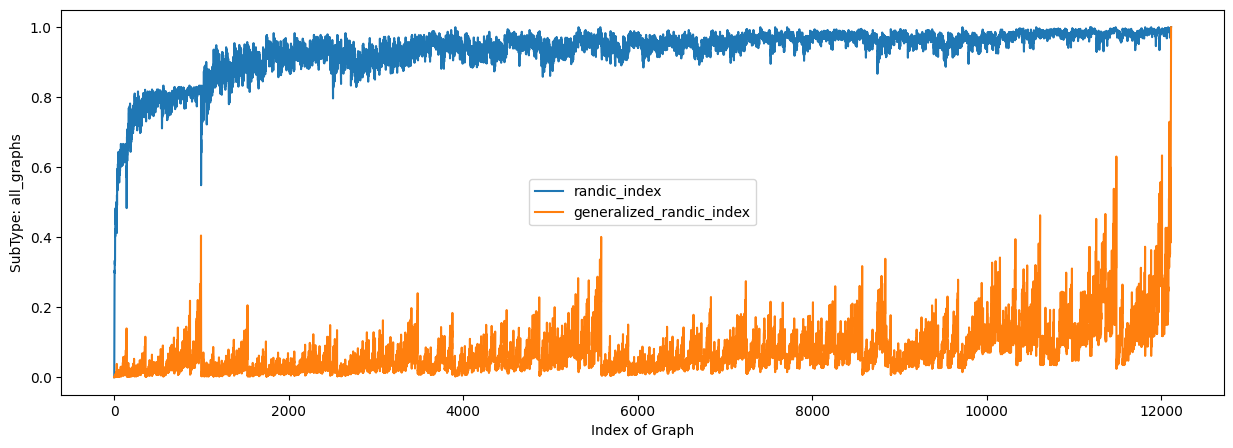
\includegraphics[width=9cm]{images/42_data/explorative_analysis_nauty.png}
    \caption{Vergleich des normalisierten Randić- und des generalisierten Randić-Index von allen non isomorphic graphs (Nauty) bis 10 Knoten}
    \label{fig:explorative_analysis}
\end{figure}


\subsection{Vergleich der topologischen Indizes}

Es werden alle topologischen Indizes, für alle Graphen berechnet, auf die Klassen aufgeteilt und normalisiert.
Die Normalisierung erfolgt durch die Methode \mintinline{python3}{StandardScaler} aus \mintinline{python3}{scikit-learn} mit $ z = (x-u) / s $.
Dabei ist $u$ der Mittelwert und $s$ die Standardabweichung der Werte.

Danach werden die Werte der topologischen Indizes auf der y-Achse und die Anzahl Knoten der Graphen auf der x-Achse visualisiert.

\noindent\hrulefill\par
\noindent\makebox[\textwidth][c]{%
    \begin{minipage}{\textwidth}
        \begin{figure}[H]
            \begin{subfigure}{.45\textwidth}
                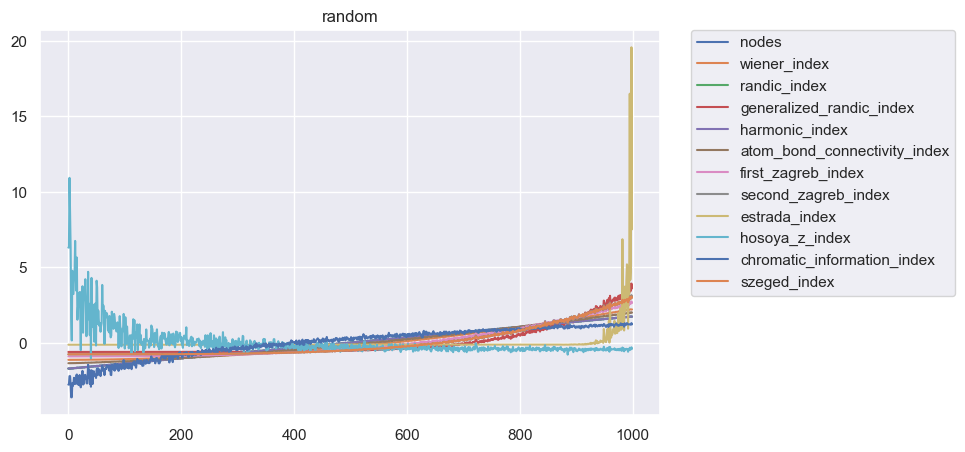
\includegraphics[width=\textwidth]{images/30_results/random-ti-comparison.png}
                \caption{Topologische Indizes der Klasse \mintinline{python3}{Random}}
                \label{fig:ti-comparison-random}
            \end{subfigure}%
            \hspace*{\fill}
            \begin{subfigure}{.45\textwidth}
                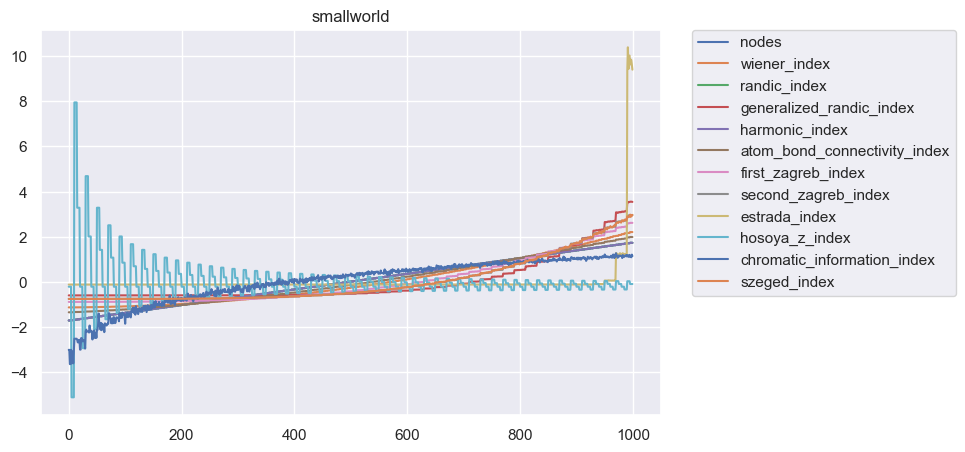
\includegraphics[width=\textwidth]{images/30_results/smallworld-ti-comparison.png}
                \caption{Topologische Indizes der Klasse \mintinline{python3}{Small-World}}
                \label{fig:ti-comparison-smallworld}
            \end{subfigure}

            \begin{subfigure}{.45\textwidth}
                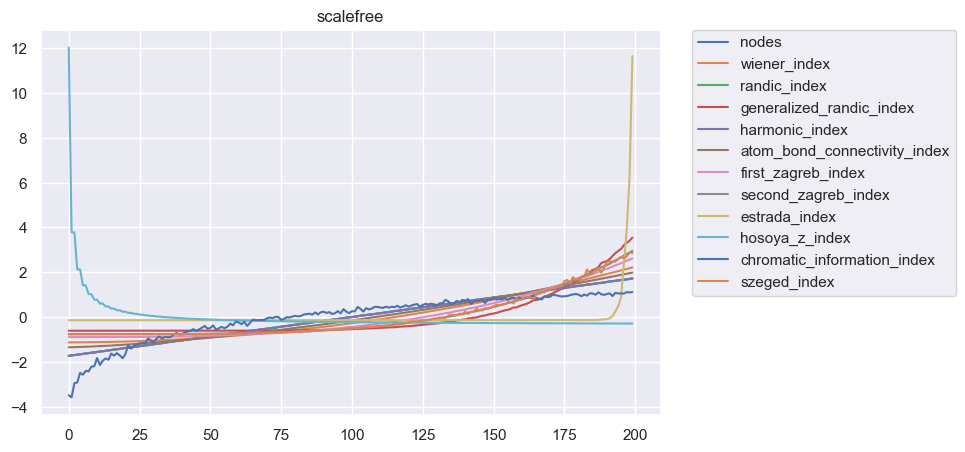
\includegraphics[width=\textwidth]{images/30_results/scalefree-ti-comparison.png}
                \caption{Topologische Indizes der Klasse \mintinline{python3}{Scale-free}}
                \label{fig:ti-comparison-scalefree}
            \end{subfigure}%
            \hspace*{\fill}
            \begin{subfigure}{.45\textwidth}
                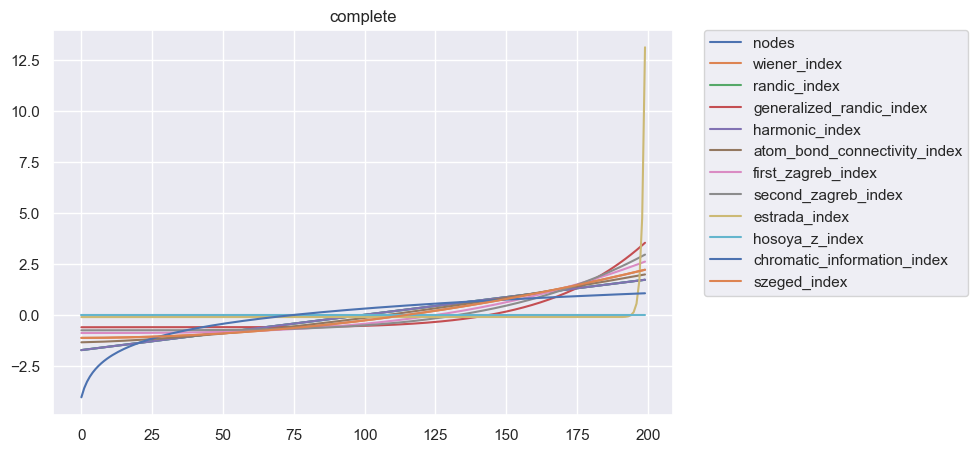
\includegraphics[width=\textwidth]{images/30_results/complete-ti-comparison.png}
                \caption{Topologische Indizes der Klasse \mintinline{python3}{Complete}}
                \label{fig:ti-comparison-complete}
            \end{subfigure}

            \begin{subfigure}{.45\textwidth}
                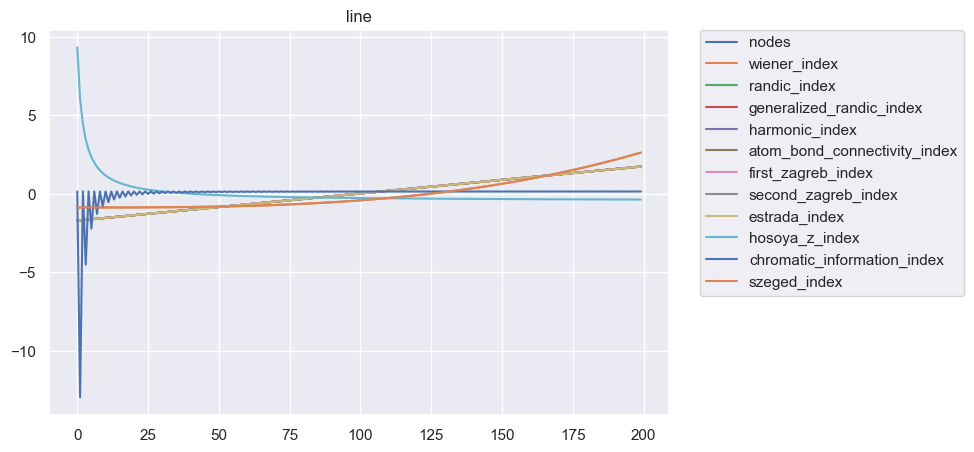
\includegraphics[width=\textwidth]{images/30_results/line-ti-comparison.png}
                \caption{Topologische Indizes der Klasse \mintinline{python3}{Line}}
                \label{fig:ti-comparison-line}
            \end{subfigure}%
            \hspace*{\fill}
            \begin{subfigure}{.45\textwidth}
                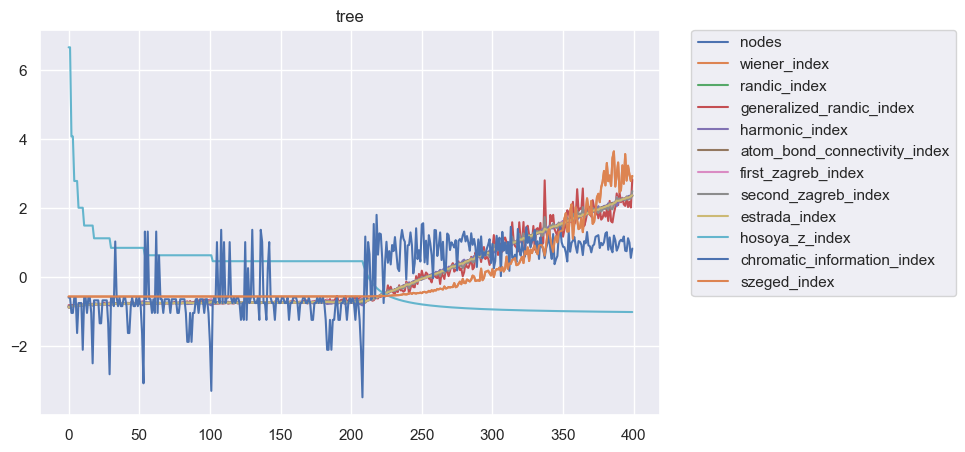
\includegraphics[width=\textwidth]{images/30_results/tree-ti-comparison.png}
                \caption{Topologische Indizes der Klasse \mintinline{python3}{Tree}}
                \label{fig:ti-comparison-tree}
            \end{subfigure}

            \center
            \begin{subfigure}{.45\textwidth}
                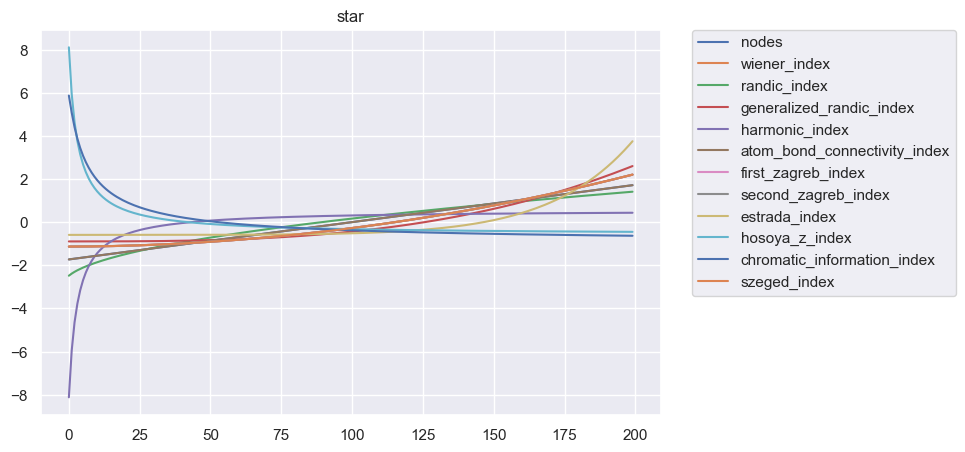
\includegraphics[width=\textwidth]{images/30_results/star-ti-comparison.png}
                \caption{Topologische Indizes der Klasse \mintinline{python3}{Star}}
                \label{fig:ti-comparison-star}
            \end{subfigure}
        \end{figure}
    \end{minipage}}

Die Abbildungen \ref{fig:ti-comparison-random} bis \ref{fig:ti-comparison-star} erhalten die normalisierten topologischen Indizes der verschiedenen Graphenklassen.
Die Resultate sind in Anhang \ref{sec:compare-ti-classes} zur besseren Lesbarkeit in grösser Form zu finden.
Bereits auf den Abbildungen ist zu erkennen, dass sich die topologischen Indizes der Graphenklassen unterscheiden. Es gibt starke Differenzen zwischen den Graphenklassen \mintinline{python3}{Random} und \mintinline{python3}{Small-World} sowie \mintinline{python3}{Scale-free} und \mintinline{python3}{Complete}.

Besonders auffallend sind die Werte der \mintinline{python3}{Tree} und \mintinline{python3}{Small-World} Klassen auf Abbildung \ref{fig:ti-comparison-tree} und \ref{fig:ti-comparison-smallworld}. Hier stechen besonders der Hosoya-Z-Index und der CII heraus, sie besitzen eine besonders hohe Varianz. Sie sind besonders sensitiv auf die Struktur der Graphenklassen bei Änderungen der Knotenzahl \cite{furtula_structure-sensitivity_2013}.

\newpage
\subsection{Korrelation der topologischen Indizes}

Um die Korrelation der topologischen Indizes zu untersuchen, werden die berechneten topologischen Indizes in einer Matrix gespeichert.
Dann werden die Korrelationsmatrizen der topologischen Indizes berechnet und in einer Heatmap geplottet.
Für die Korrelation wird die Spearman-Korrelation \cite{spearman_proof_1904} verwendet.

Diese weist, wie die Pearson-Korrelation, der Korrelation von zwei Variablen einen Wert zwischen -1 und 1 zu. Dabei ist -1 eine vollständige negative Korrelation, 0 bedeutet vollständige unkorrelierte Variablen und 1 eine vollständige positive Korrelation. Die Spearman-Korrelation ist Ausreissern gegenüber weniger empfindlich als die Pearson-Korrelation \cite[p.~73ff]{bartl_statistik_2017}.

In Anhang \ref{sec:correlation-pairs} werden zusätzlich zu den Heatmaps die einzelnen Werte in einem 2D-Scatterplot visualisiert miteinander verglichen. Um die topologischen Indizes besser zu verstehen, wurde entschieden, die topologischen Indizes für eine Klasse auch einzeln zu vergleichen.
Dazu folgen als Nächstes die Zusammenhänge aller topologischen Indizes untereinander.

\begin{figure}[H]
    \centering
    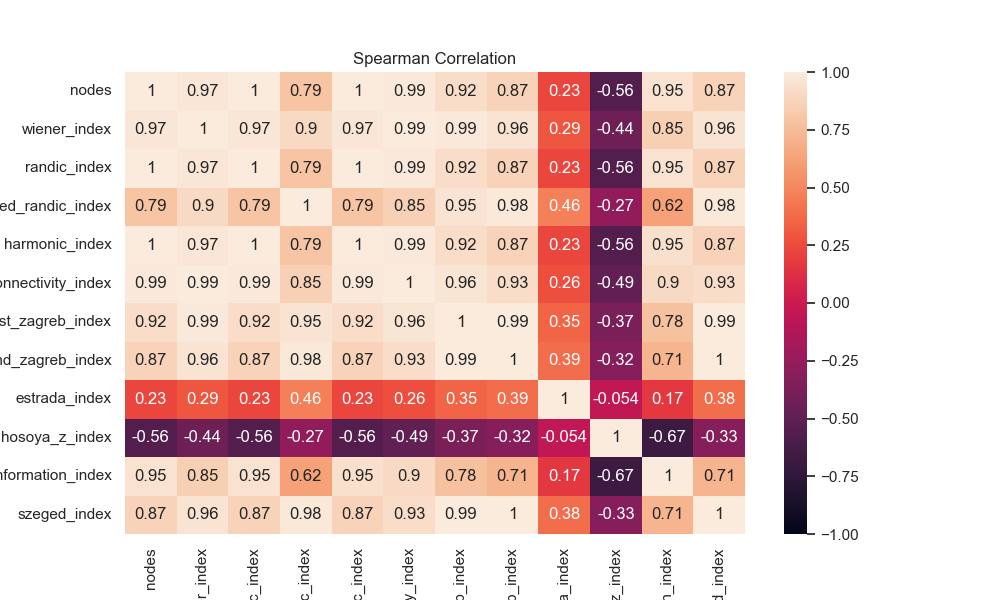
\includegraphics[width=0.8\textwidth]{images/30_results/random-correlation.png}
    \caption{Spearman-Korrelation der topologischen Indizes der Klasse \mintinline{python3}{Random}}
    \label{fig:correlation-random}
\end{figure}

Anhand von Abbildung \ref{fig:correlation-random} kann festgestellt werden, dass zwei topologische Indizes einen fast unkorrelierten Zusammenhang haben. Es handelt sich dabei um die des Estrada-Index und des Hosoya-Z-Index. Ihre Werte liegen zwischen $ -0.67 $ und $ 0.45 $, wobei die meisten Werte nahe um $ 0 $ sind.

Ebenfalls auffallend ist, dass alle anderen topologischen Indizes eine positive Korrelation aufweisen. Auch wenn diese nicht überall besonders hoch ist, ist sie trotzdem generell positiv.

\begin{figure}[H]
    \centering
    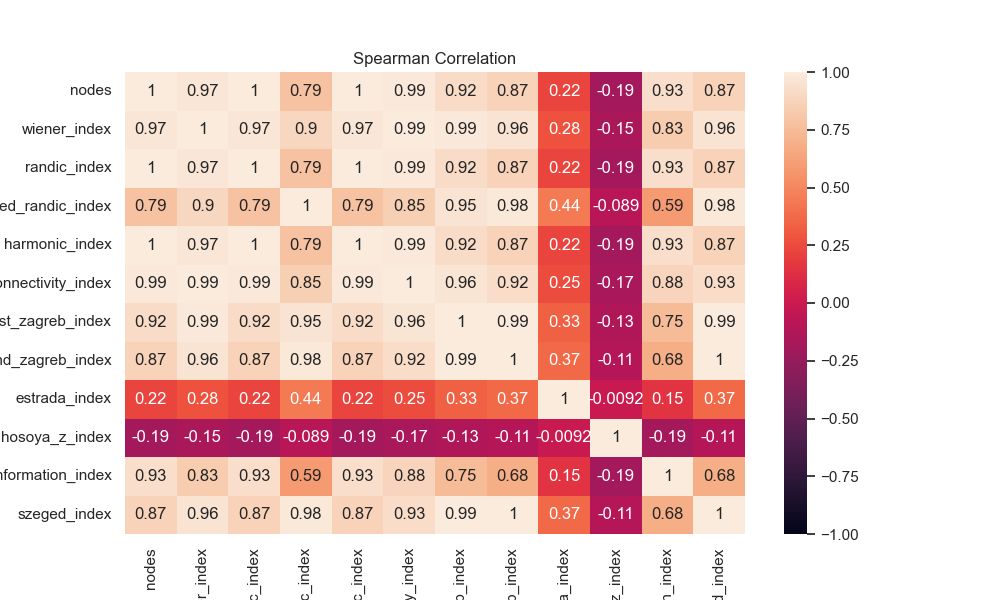
\includegraphics[width=0.8\textwidth]{images/30_results/smallworld-correlation.png}
    \caption{Spearman-Korrelation der topologischen Indizes der Klasse \mintinline{python3}{Small-World}}
    \label{fig:correlation-smallworld}
\end{figure}

\begin{figure}[H]
    \centering
    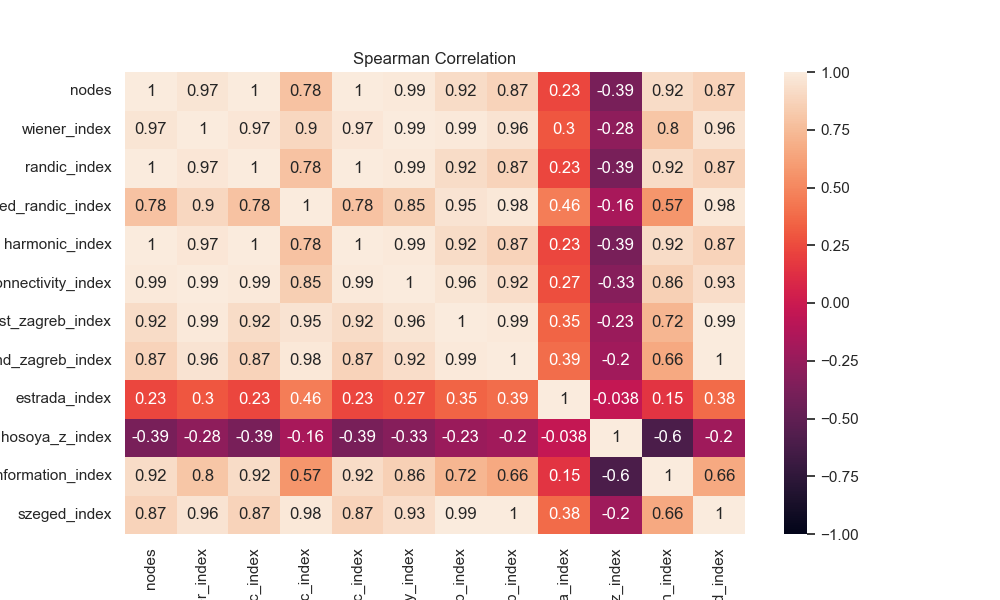
\includegraphics[width=0.8\textwidth]{images/30_results/scalefree-correlation.png}
    \caption{Spearman-Korrelation der topologischen Indizes der Klasse \mintinline{python3}{Scale-free}}
    \label{fig:correlation-scalefree}
\end{figure}

Die Spearman-Korrelation für die Random-Graphen nach Erdős-Rényi, die Small-World-Graphen nach Watts-Strogatz und die Scale-free-Graphen nach Barabási-Albert sind auf den ersten Blick fast identisch. Ihre Heatplots liefern fast identische Ergebnisse.

Die Korrelation des Estrada- und die des Hosoya-Z-Index sind bei den Small-World- und Scale-free-Klassen noch näher bei $ 0 $ als bei den Erdős-Rényi-Graphen.

\begin{figure}[H]
    \centering
    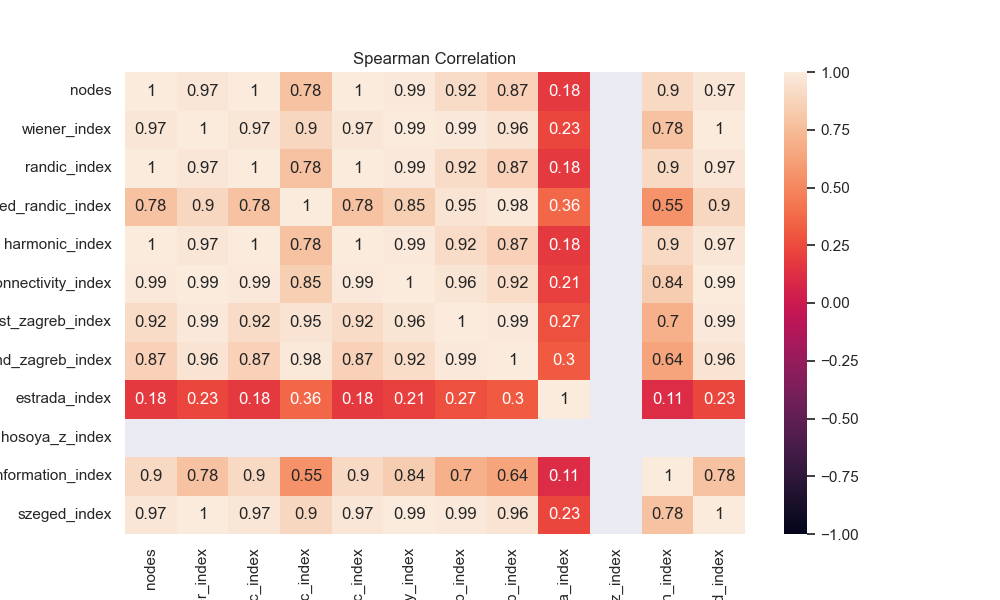
\includegraphics[width=0.7\textwidth]{images/30_results/complete-correlation.png}
    \caption{Spearman-Korrelation der topologischen Indizes der Klasse \mintinline{python3}{Complete}}
    \label{fig:correlation-complete}
\end{figure}

Die Complete-Graphen liefern eine besondere Korrelation. Der Hosoya-Z-Index ist, wie in der Theorie \ref{sec:hosoya_index} beschrieben, bei den Complete-Graphen immer das Maximum.
Neben dem Estrada-Index, welcher ebenfalls wieder nahe bei $ 0 $ liegt, fällt der Szeged-Index auf. Dieser korreliert im Durchschnitt am stärksten mit den anderen topologischen Indizes.

\begin{figure}[H]
    \centering
    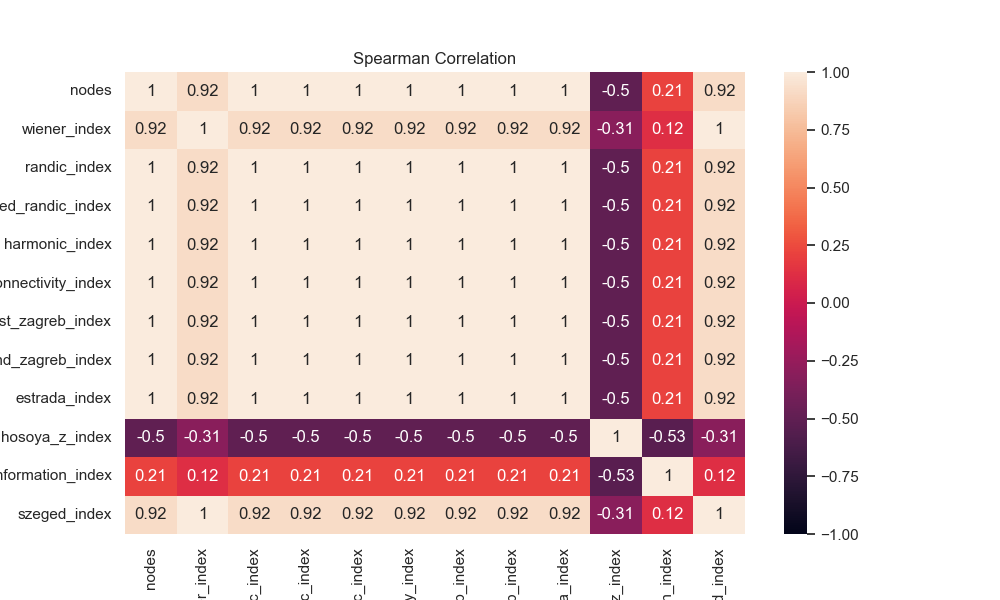
\includegraphics[width=0.7\textwidth]{images/30_results/line-correlation.png}
    \caption{Spearman-Korrelation der topologischen Indizes der Klasse \mintinline{python3}{Line}}
    \label{fig:correlation-line}
\end{figure}

Die Pfadgraphen liefern eine monoton aufsteigende Korrelation. Ebenfalls in Anhang \ref{sec:correlation-pairs} ist zu erkennen, dass die Werte der topologischen Indizes der Klasse \mintinline{python3}{Line} überaus ähnlich sind. Ihr $r$- und $p$-Wert liegt bei fast allen Indizes bei $1$.

\begin{figure}[H]
    \centering
    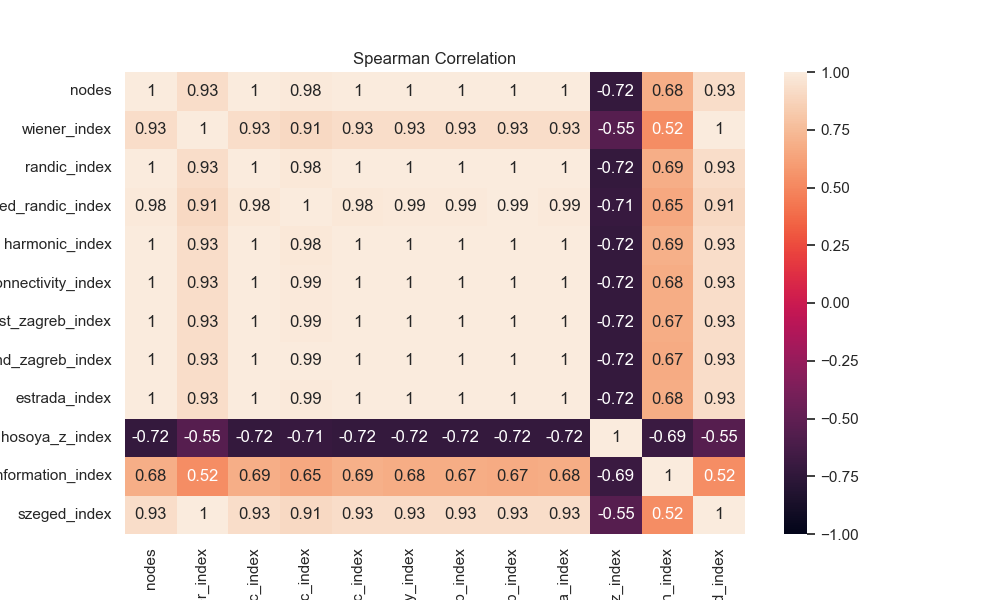
\includegraphics[width=0.7\textwidth]{images/30_results/tree-correlation.png}
    \caption{Spearman-Korrelation der topologischen Indizes der Klasse \mintinline{python3}{Tree}}
    \label{fig:correlation-tree}
\end{figure}

Die Baumgraphen liefern eine ähnliche Korrelation wie die Pfadgraphen. Auch hier ist festzustellen, dass die Werte der topologischen Indizes der Klasse \mintinline{python3}{Tree} überaus ähnlich sind. Neu zu erkennen ist jedoch der abfallende Trend beim CII und dem Hosoya-Z-Index. Dieser Trend ist auch in Anhang \ref{sec:correlation-pairs} zu sehen. Der Wiener-Index verhält sich zum Szeged-Index in etwa gleich.

\begin{figure}[H]
    \centering
    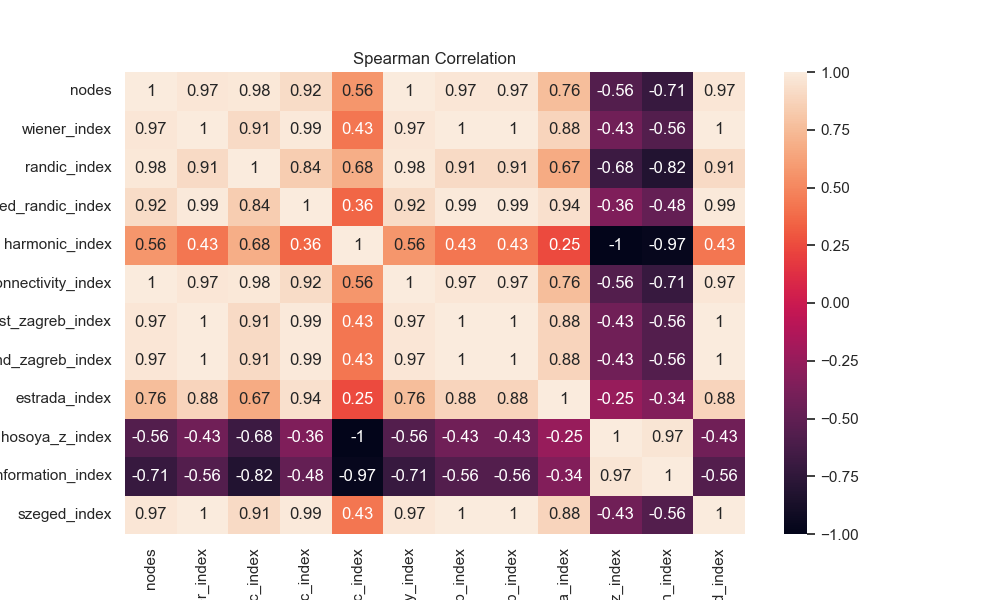
\includegraphics[width=0.7\textwidth]{images/30_results/star-correlation.png}
    \caption{Spearman-Korrelation der topologischen Indizes der Klasse \mintinline{python3}{Star}}
    \label{fig:correlation-star}
\end{figure}

Die Sterngraphenklasse liefert ein neues Bild der Heatmap. Im Durchschnitt korreliert der ABC-Index am stärksten monoton aufsteigend mit den anderen topologischen Indizes. Besonders deutlich zu sehen, ist die Korrelation aller topologischen Indizes untereinander; es gibt keine Werte, welche sich durchgehend nahe bei $0$ befinden.

\newpage

\subsection{Principal Component Analysis}

Die Principal Component Analysis (PCA) ist eine statistische Methode, mit welcher die Dimensionalität von Daten reduziert \cite{jolliffe_principal_1986} wird.
Dabei werden die Daten in eine neue Basis transformiert, welche die maximale Varianz der Daten wiedergibt.
Mathematisch wird dies durch die Eigenwerte und Eigenvektoren der Kovarianzmatrix der Daten beschrieben.

\subsubsection{Beitrag der PCA zur Usefulness}

Die PCA kann verwendet werden, um einen Datensatz aus interdependenten Variablen in einen neuen Satz von Variablen, den Hauptkomponenten, zu transformieren \cite{jolliffe_principal_1986}.
Diese Hauptkomponenten können dann analysiert werden, um Trends, Sprünge, Cluster und Ausreisser in den Daten zu beobachten.
Durch die Verwendung der PCA-Methode können wir die Nützlichkeit von topologischen Indizes für verschiedene Klassen von Graphen vergleichen.
Die PCA kann uns helfen, die wichtigsten Hauptkomponenten zu identifizieren, die zur Unterscheidung zwischen den verschiedenen Klassen von Graphen beitragen.
Auf diese Weise können wir die topologischen Indizes identifizieren, die für die verschiedenen Klassen von Graphen am nützlichsten sind.

Durch die Anwendung der PCA können die topologischen Indizes, die die grösste Varianz innerhalb der Daten erklären, identifiziert werden und somit wichtige Informationen über die Struktur der Graphen liefern \cite[p.~303]{basak_topological_1987}.

Im Jahr 1987 haben Basak et al. 90 Indizes mittels PCA auf ihre aussagekräftigste Komponente reduziert \cite{basak_topological_1987}.
Sie sind zum Resultat gekommen, dass die ersten zehn Komponenten 90 \% der Varianz der Daten beschreiben.

Durch die Anwendung der PCA auf die topologischen Indizes können die Hauptkomponenten identifiziert werden, die die meisten Informationen enthalten und somit am meisten zur Beschreibung der Struktur des Netzwerks beitragen.
Die \textbf{\textit{Usefulness}} der topologischen Indizes wird in dieser Arbeit gemessen, indem die Hauptkomponenten mit den höchsten Eigenwerten identifiziert werden.
Somit können die topologischen Indizes identifiziert werden, die die meisten Informationen enthalten und somit am meisten zur Beschreibung der Struktur des Netzwerks beitragen.
Auf diese Weise können die wichtigsten topologischen Indizes für verschiedene Klassen von Graphen identifiziert werden.

\subsubsection{PCA in scikit-learn}

Um die PCA etwas besser verstehen zu können, wird zuerst das eingegebene Datenset in einem 2D-Plot visualisiert.
Die PCA-Methode in \mintinline{python3}{scikit-learn} wurde per Randomized Singular Value Decomposition (SVD) implementiert \cite{halko_finding_2011}.
Diese Methode wird automatisch von der PCA-Methode in scikit-learn verwendet, wenn ein grosses Datenset ($> 500 \times 500$) eingegeben wird.

\subsubsection{Erklärbare Varianz}

Es wird untersucht, wie viele Principal Components (PCs) benötigt werden, um 95 \% der Varianz der Daten zu beschreiben.
Dies kann mit einem Scree-Plot dargestellt werden, der auf der x-Achse die Anzahl der PCs und auf der y-Achse die Varianz der Daten hat, welche durch die PCs beschrieben wird.

\begin{figure}[H]
    \begin{subfigure}{.5\textwidth}
        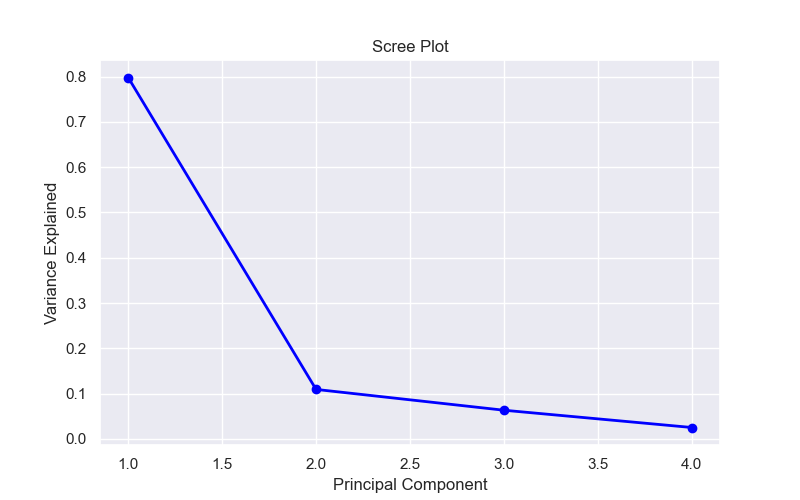
\includegraphics[width=\textwidth]{images/30_results/random-scree.png}
        \caption{Scree Plot stellt die Varianz der PC in \mintinline{python3}{Random} dar}
        \label{fig:scree-random}
    \end{subfigure}%
    \begin{subfigure}{.5\textwidth}
        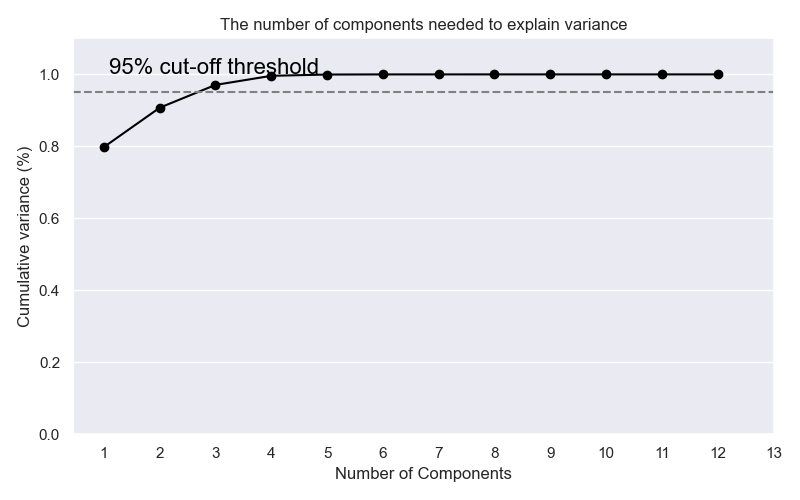
\includegraphics[width=\textwidth]{images/30_results/random-scree-cum.png}
        \caption{Scree Plot stellt die kumulative Varianz der PC in \mintinline{python3}{Random} dar}
        \label{fig:scree-cum-random}
    \end{subfigure}
\end{figure}

\medskip

\begin{figure}
    \ContinuedFloat
    \begin{subfigure}{.5\textwidth}
        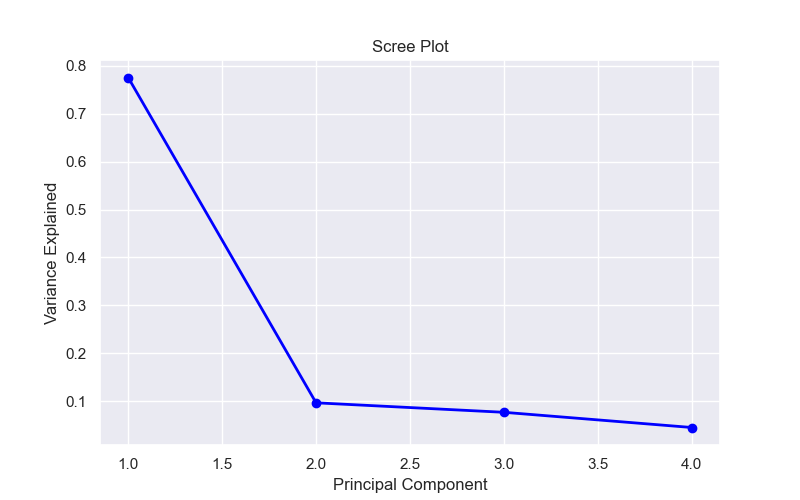
\includegraphics[width=\textwidth]{images/30_results/smallworld-scree.png}
        \caption{Scree Plot stellt die Varianz der PC in \mintinline{python3}{Small-World} dar}
        \label{fig:scree-smallworld}
    \end{subfigure}%
    \begin{subfigure}{.5\textwidth}
        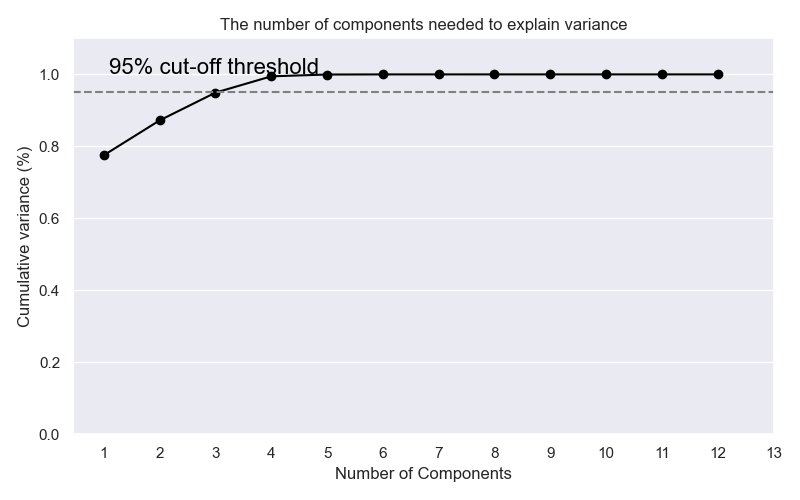
\includegraphics[width=\textwidth]{images/30_results/smallworld-scree-cum.png}
        \caption{Scree Plot stellt die kumulative Varianz der PC in \mintinline{python3}{Small-World} dar}
        \label{fig:scree-cum-smallworld}
    \end{subfigure}

    \begin{subfigure}{.5\textwidth}
        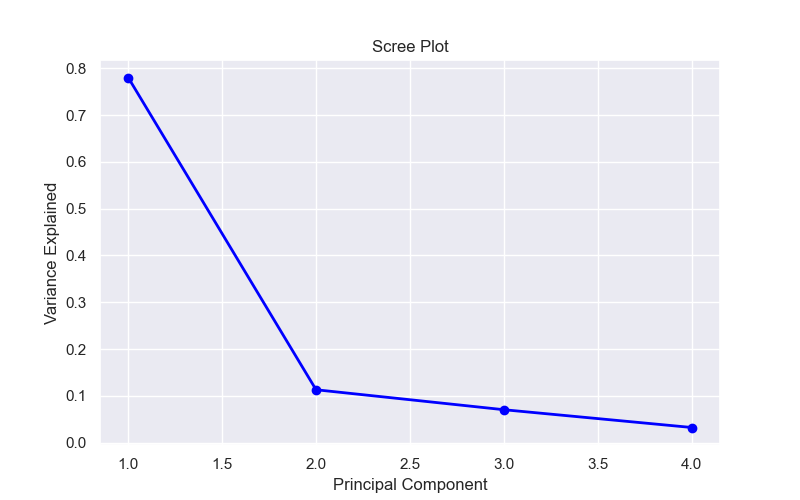
\includegraphics[width=\textwidth]{images/30_results/scalefree-scree.png}
        \caption{Scree Plot stellt die Varianz der PC in \mintinline{python3}{Scale-free} dar}
        \label{fig:scree-scalefree}
    \end{subfigure}%
    \begin{subfigure}{.5\textwidth}
        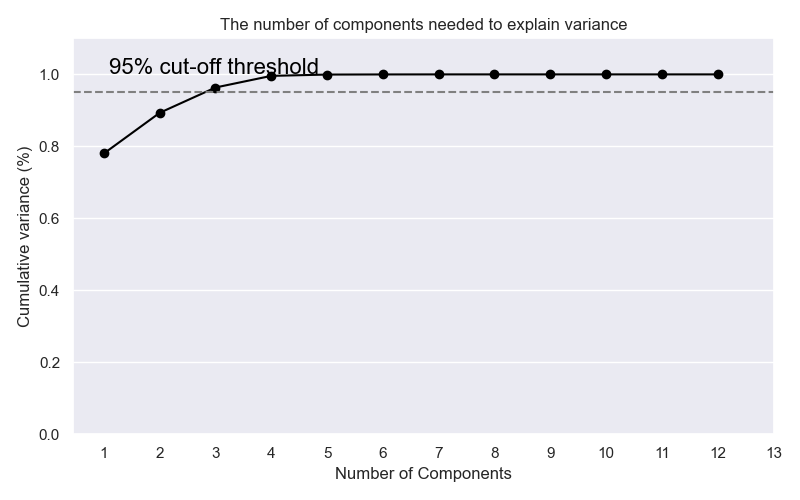
\includegraphics[width=\textwidth]{images/30_results/scalefree-scree-cum.png}
        \caption{Scree Plot stellt die kumulative Varianz der PC in \mintinline{python3}{Scale-free} dar}
        \label{fig:scree-cum-scalefree}
    \end{subfigure}
    \ContinuedFloat
    \begin{subfigure}{.5\textwidth}
        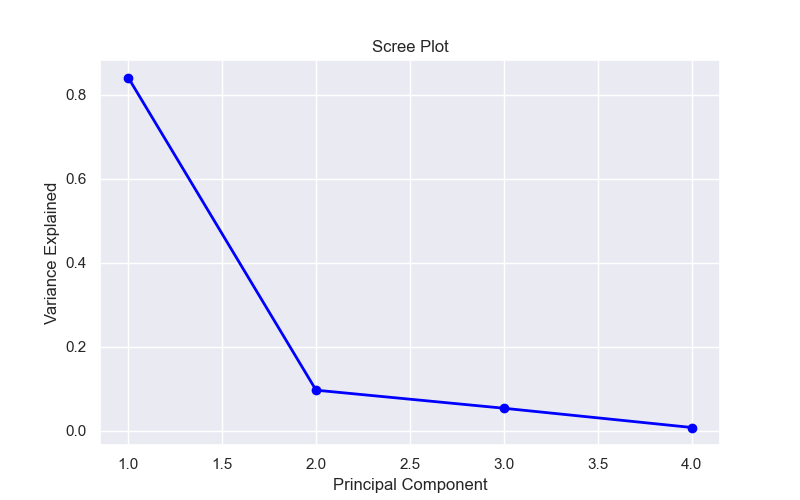
\includegraphics[width=\textwidth]{images/30_results/complete-scree.png}
        \caption{Scree Plot stellt die Varianz der PC in \mintinline{python3}{Complete} dar}
        \label{fig:scree-complete}
    \end{subfigure}%
    \begin{subfigure}{.5\textwidth}
        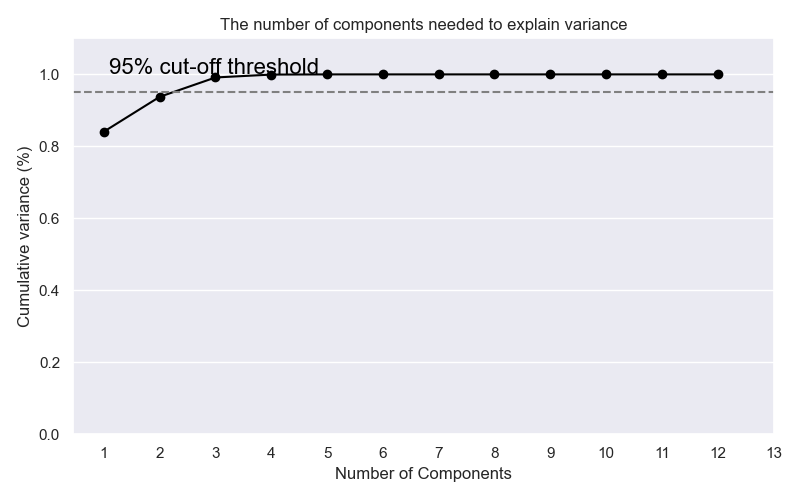
\includegraphics[width=\textwidth]{images/30_results/complete-scree-cum.png}
        \caption{Scree Plot stellt die kumulative Varianz der PC in \mintinline{python3}{Complete} dar}
        \label{fig:scree-cum-complete}
    \end{subfigure}
\end{figure}

\medskip

\begin{figure}
    \ContinuedFloat
    \begin{subfigure}{.5\textwidth}
        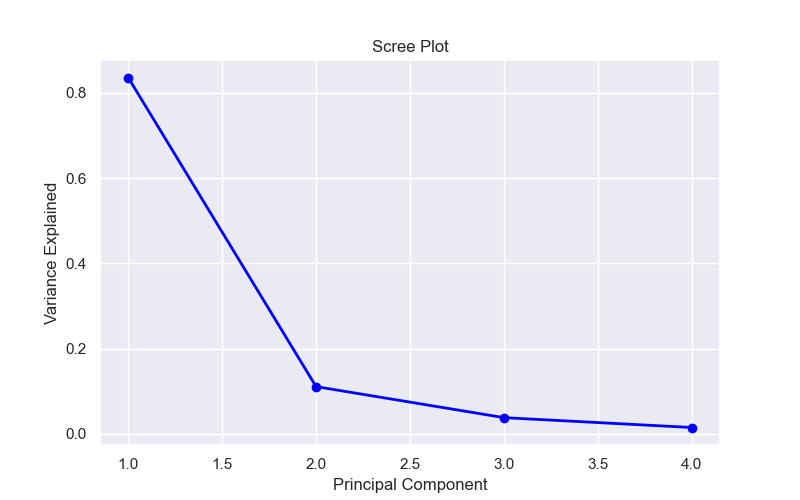
\includegraphics[width=\textwidth]{images/30_results/line-scree.png}
        \caption{Scree Plot stellt die Varianz der PC in \mintinline{python3}{Line} dar}
        \label{fig:scree-line}
    \end{subfigure}%
    \begin{subfigure}{.5\textwidth}
        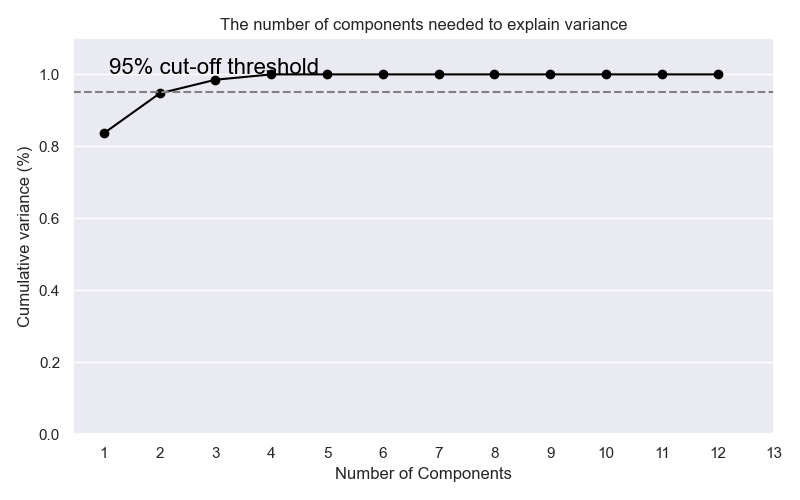
\includegraphics[width=\textwidth]{images/30_results/line-scree-cum.png}
        \caption{Scree Plot stellt die kumulative Varianz der PC in \mintinline{python3}{Line} dar}
        \label{fig:scree-cum-line}
    \end{subfigure}

    \begin{subfigure}{.5\textwidth}
        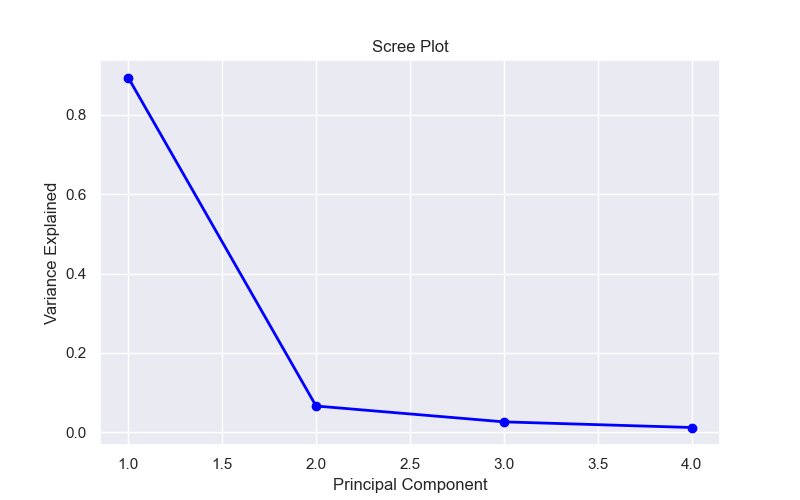
\includegraphics[width=\textwidth]{images/30_results/tree-scree.png}
        \caption{Scree Plot stellt die Varianz der PC in \mintinline{python3}{Tree} dar}
        \label{fig:scree-tree}
    \end{subfigure}%
    \begin{subfigure}{.5\textwidth}
        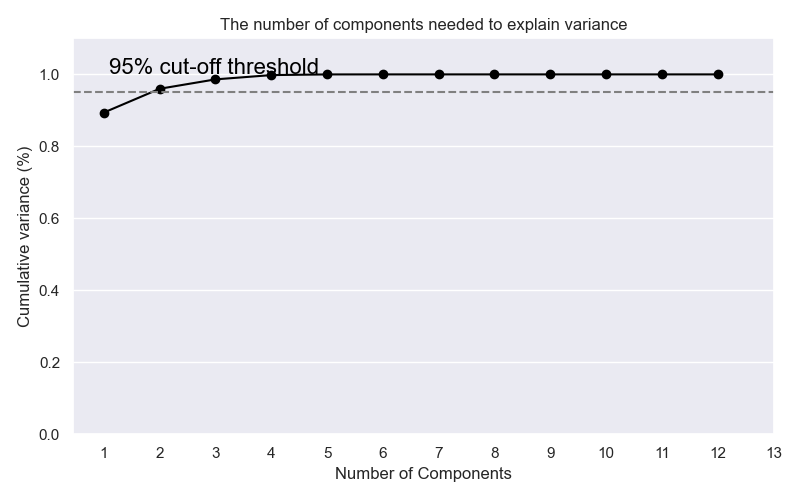
\includegraphics[width=\textwidth]{images/30_results/tree-scree-cum.png}
        \caption{Scree Plot stellt die kumulative Varianz der PC in \mintinline{python3}{Tree} dar}
        \label{fig:scree-cum-tree}
    \end{subfigure}

    \begin{subfigure}{.5\textwidth}
        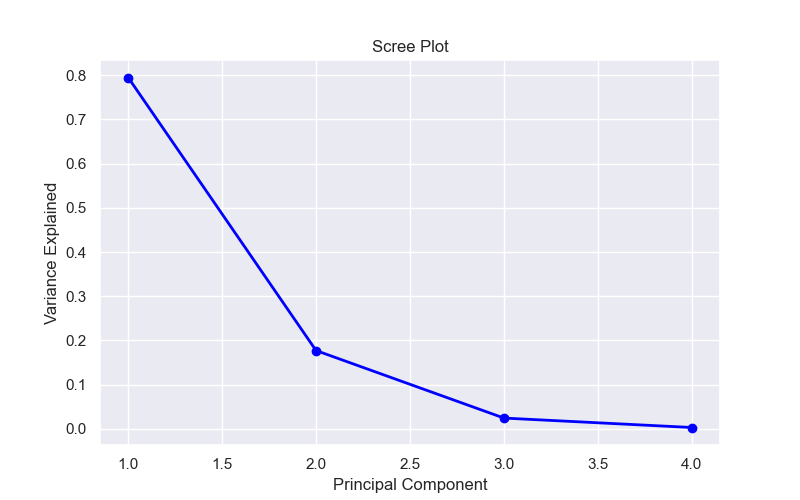
\includegraphics[width=\textwidth]{images/30_results/star-scree.png}
        \caption{Scree Plot stellt die Varianz der PC in \mintinline{python3}{Star} dar}
        \label{fig:star-line}
    \end{subfigure}%
    \begin{subfigure}{.5\textwidth}
        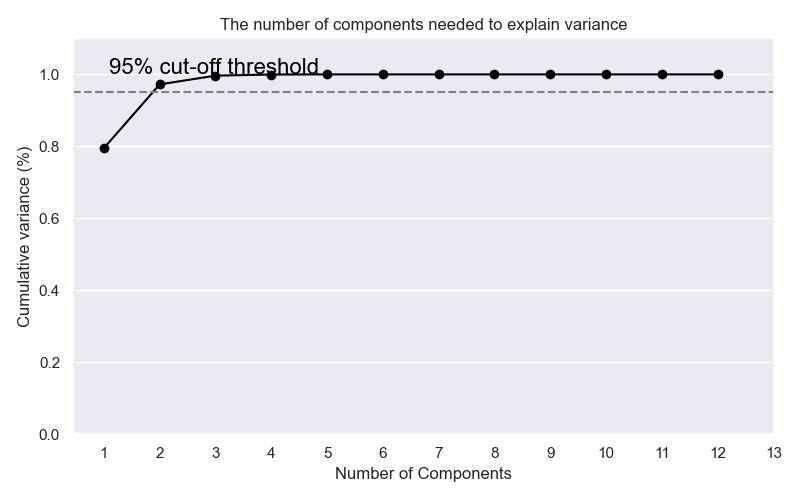
\includegraphics[width=\textwidth]{images/30_results/star-scree-cum.png}
        \caption{Scree Plot stellt die kumulative Varianz der PC in \mintinline{python3}{Star} dar}
        \label{fig:scree-cum-star}
    \end{subfigure}
\end{figure}

Auf allen Abbildung von \ref{fig:scree-random} bis \ref{fig:scree-cum-star} ist zu erkennen, dass die Varianz der ersten Komponente überaus hoch ist. Die erklärbare Varianz von 95 \% wird in allen Klassen mit maximal vier Komponenten erreicht. In den meisten Klassen reichen zwei Komponenten aus.
Bei den Baum- und Sterngraphen genügt sogar eine Komponente, um 95 \% der Varianz zu erklären.

\newpage

\paragraph{PCA-Loadings}

Als Nächstes folgen die Loadings der PCA-Methode. Die Eigenvektoren der PCs geben die Richtung der Komponenten an, während die Eigenwerte die Varianz der Komponenten beschreiben.
Die Loadings, auch $Q$-Matrix genannt, sind die Gewichte der einzelnen Variablen, welche die Komponenten beschreiben \cite[p.~434]{abdi_principal_2010}.
Im Wesentlichen zeigen die Loadings, wie stark jede Variable mit jeder der Hauptkomponenten korreliert. Hohe positive Loadings zeigen an, dass eine Variable stark mit einer bestimmten Hauptkomponente korreliert, während hohe negative Loadings anzeigen, dass die Variable eine starke negative Korrelation mit der Hauptkomponente aufweist.
Die Loadings können verwendet werden, um zu verstehen, welche Variablen in den Daten am meisten zur Variabilität beitragen und wie die Variablen miteinander zusammenhängen \cite[p.~438]{abdi_principal_2010}.

Sie werden nachfolgend in einem 2D-Plot visualisiert, wobei die x-Achse die erste Komponente und die y-Achse die zweite Komponente wiedergibt, und Folgendermassen berechnet:

\begin{equation}
    \label{eq:loadings}
    \text{Loadings} = \text{Eigenvektoren} \cdot \sqrt{\text{Eigenwerte}}
\end{equation}

\begin{figure}[H]
    \centering
    \begin{subfigure}{.5\textwidth}
        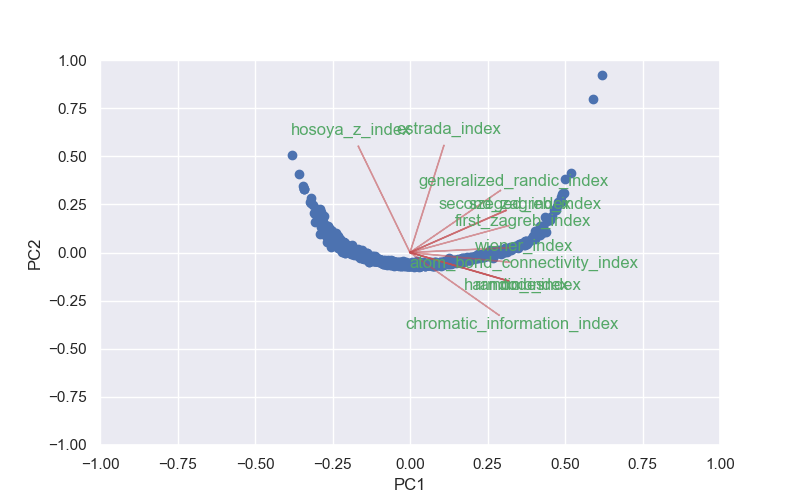
\includegraphics[width=\textwidth]{images/30_results/random-pca-loadings.png}
        \caption{Loading Plots der 2-PCA Methode der Klasse \mintinline{python3}{Random}}
        \label{fig:pca-loading-random}
    \end{subfigure}%
    \begin{subfigure}{.5\textwidth}
        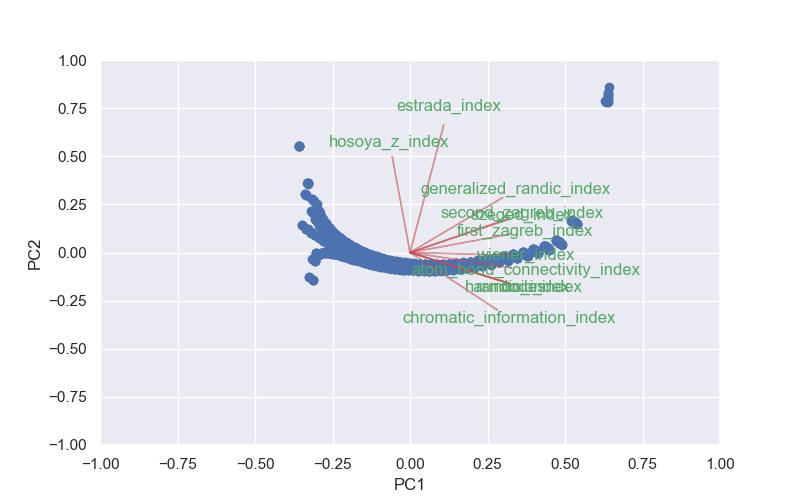
\includegraphics[width=\textwidth]{images/30_results/smallworld-pca-loadings.png}
        \caption{Loading Plots der 2-PCA Methode der Klasse \mintinline{python3}{Small-World}}
        \label{fig:pca-loading-smallworld}
    \end{subfigure}

    \begin{subfigure}{.5\textwidth}
        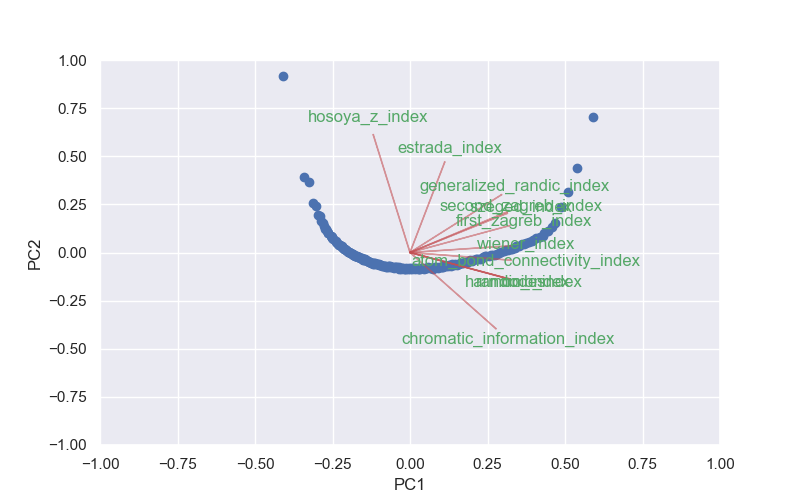
\includegraphics[width=\textwidth]{images/30_results/scalefree-pca-loadings.png}
        \caption{Loading Plots der 2-PCA Methode der Klasse \mintinline{python3}{Scale-free}}
        \label{fig:pca-loading-scalefree}
    \end{subfigure}%
    \begin{subfigure}{.5\textwidth}
        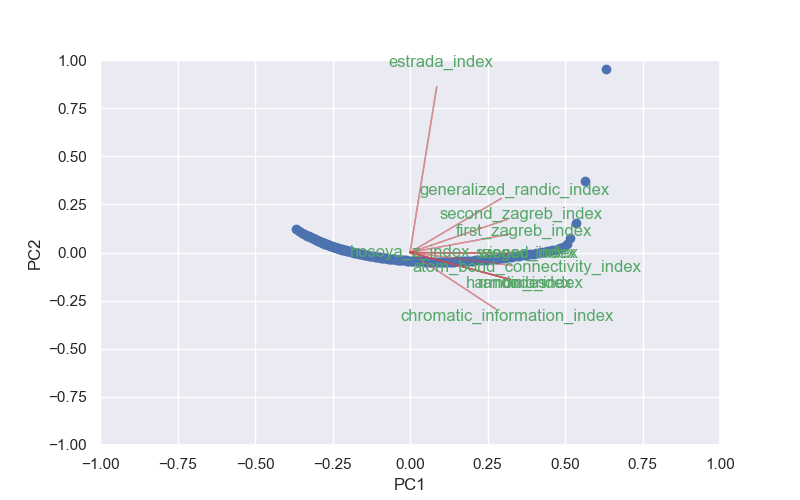
\includegraphics[width=\textwidth]{images/30_results/complete-pca-loadings.png}
        \caption{Loading Plots der 2-PCA Methode der Klasse \mintinline{python3}{Complete}}
        \label{fig:pca-loading-complete}
    \end{subfigure}
\end{figure}


\begin{figure}[H]
    \ContinuedFloat
    \centering
    \begin{subfigure}{.5\textwidth}
        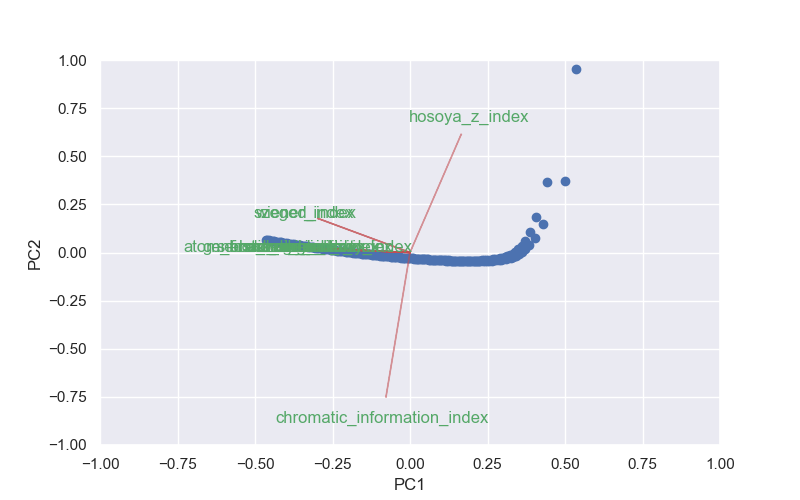
\includegraphics[width=\textwidth]{images/30_results/line-pca-loadings.png}
        \caption{Loading Plots der 2-PCA Methode der Klasse \mintinline{python3}{Line}}
        \label{fig:pca-loading-line}
    \end{subfigure}%
    \begin{subfigure}{.5\textwidth}
        \includegraphics[width=\textwidth]{images/30_results/tree-pca-loadings.png}
        \caption{Loading Plots der 2-PCA Methode der Klasse \mintinline{python3}{Tree}}
        \label{fig:pca-loading-tree}
    \end{subfigure}
\end{figure}

\begin{figure}[H]
    \ContinuedFloat
    \centering
    \begin{subfigure}{0.8\textwidth}
        \centering
        \includegraphics[width=0.8\textwidth]{images/30_results/star-pca-loadings.png}
        \caption{Loading Plots der 2-PCA Methode der Klasse \mintinline{python3}{Star}}
        \label{fig:pca-loading-star}
    \end{subfigure}%
\end{figure}

Die Loadings der PCs zeigen, wie die topologischen Indizes zur Komponente beitragen.
Ähnlich wie bei der Spearman-Korrelation bedeuten positive Loadings, dass der Index eine positive Korrelation zur Komponente hat; negative Loadings entsprechen einer negativen Korrelation. Je höher der Wert ist, desto stärker ist die Korrelation \cite{bartl_statistik_2017}. Für uns bedeutet das, dass die Indizes mit hohen positiven Loadings die Komponente stark beeinflussen.

Die Eigenwerte $ \lambda $ der Komponenten speichern die Varianz der Komponenten und die Eigenvektoren $ \vec{v} $ die Richtung der Komponenten. Werden nun $ \lambda $ auf $ \vec{v} $ übertragen, so erhält man die PC-Loadings. Diese Loadings enthalten, da sie Varianz als auch Richtung enthalten, die Kovarianz zwischen den ursprünglichen Werten und den PCs \cite[p.~438]{abdi_principal_2010}.

\newpage

\subsubsection{Einfluss der Komponenten}

Zum Schluss der Korrelationsanalyse werden die einzelnen Komponenten der PCA-Methode der jeweiligen Klassen identifiziert.
Mittels der den Scree-Plots lässt sich feststellen, dass bei den überwiegenden Klassen die ersten zwei Komponenten die meisten Informationen über die Daten enthalten.
Deshalb werden die einzelnen Komponenten der Klasse \mintinline{python3}{Random} bei den Hauptkomponenten zur Analyse ausgegeben.

\begin{table}[H]
    \caption{PCA-Komponenten der Erdős-Rényi-Klasse und der Einfluss der Indizes auf die Komponenten}
    \begin{adjustbox}{minipage=\textwidth, center}
        \tiny
        \begin{tabularx}{\textwidth}{l c c c c c c c c c c c}
            \hline
                          & wiener         & randic & g. randic & harmonic & abc    & 1st zagreb & 2nd zagreb & estrada        & z              & cii    & szeged \\ \hline
            \textbf{PC-1} & \textbf{0.338} & 0.331  & 0.310     & 0.331    & 0.337  & 0.334      & 0.327      & 0.119          & -0.172         & 0.297  & 0.327  \\
            \textbf{PC-2} & 0.007          & -0.165 & 0.303     & -0.165   & -0.068 & 0.121      & 0.200      & 0.554          & \textbf{0.575} & -0.342 & 0.198  \\
            \textbf{PC-3} & -0.113         & -0.019 & -0.075    & -0.019   & -0.077 & -0.131     & -0.123     & \textbf{0.784} & -0.544         & 0.128  & -0.127 \\
            \textbf{PC-4} & 0.057          & 0.258  & -0.379    & 0.258    & 0.166  & -0.103     & -0.230     & 0.239          & \textbf{0.576} & 0.431  & -0.235 \\ \hline
        \end{tabularx}
    \end{adjustbox}
    \label{table:pca_components}
\end{table}

In Tabelle \ref{table:pca_components} ist der Einfluss der Variablen (hier topologische Indizes) auf die Komponenten der Klasse \mintinline{python3}{Random} dargestellt.
Es ist ersichtlich, dass der Wiener-Index den stärksten Einfluss auf die erste Hauptkomponente hat, der Hosoya-Z-Index auf die zweite und vierte und der Estrada-Index auf die dritte Komponente.
Die abschliessende Liste aller Einflüsse der topologischen Indizes auf die Komponenten der Klassen ist in Anhang \ref{sec:ti-pca} ersichtlich.

Die Tabelle \ref{table:pca_components} zeigt die Loadings der Hauptkomponenten für die Klasse \mintinline{python3}{Random}. Anhand dieser Loadings kann die Einflüsse der verschiedenen topologischen Indizes auf die Hauptkomponenten dieser Klasse bestimmt werden. Der Index mit dem höchsten Einfluss ist schliesslich der nützlichste Index für diese Klasse. Die Herleitung dieser Aussage wird anhand der Definition \ref{thm:useful_index} und der darauffolgenden Beschreibung gezeigt.

\subsubsection{Meine Definition des \textit{nützlichen} topologischen Index}

Somit ist es nun möglich, die Hauptdefinition und Beantwortung der Forschungsfrage 1 und 2 zu finden.

\begin{theorem}[\textbf{nützlicher} topologischer Index $\Phi$]
    \label{thm:useful_index}%
    Je höher der Einfluss eines topologischen Index auf die Hauptkomponenten seiner Klasse ist, desto höher ist dessen \textbf{Usefulness}.
\end{theorem}

Für dieses Theorem muss definiert werden, was mit \textit{Einfluss} gemeint ist.
Der Einfluss eines topologischen Index auf die PCs einer Klasse lässt sich anhand der Loadings der Komponenten bestimmen.
Sind die Loadings eines Index hoch positiv, so korreliert der Index positiv mit der Komponente.
Die Loading-Werte der Komponenten werden in Tabelle \ref{table:pca_components} für die Klasse \mintinline{python3}{Random} dargestellt.

Die Formel zur Berechnung der Usefulness eines topologischen Index auf die Hauptkomponenten seiner Klasse kann wie folgt definiert werden:

\begin{equation}
    \label{eq:index_usefulness}
    \Phi_{i} = \sum_{j=1}^{m} |w_{ij}| \cdot \sigma^2_j
\end{equation}

Wobei $i$ dem Index des topologischen Indizes in dem Datenset entspricht, $m$ der Anzahl der Hauptkomponenten und $j$ die $j$-te Hauptkomponente. $w_{ij}$ ist das Loading des topologischen Indizes $i$ auf der $j$-ten Hauptkomponente.
Die Werte der Loadings $w_{ij}$ werden mit der $j$-ten Hauptkomponente aufsummiert und diese danach  mit der erklärbaren Varianz $\sigma^2$ der $j$-ten Hauptkomponente multipliziert.

Die erklärbare Varianz $\sigma^2$ der Hauptkomponenten für die Klasse \mintinline{python3}{Random} lautet:

% Mint Code-Listing
\begin{listing}[H]
    \begin{minted}
    [frame=lines,framesep=2mm,baselinestretch=1.2,bgcolor=LightGray,fontsize=\footnotesize,linenos]
    {text}    
------------ PCA random 4 explained variance ratio ------------
        explained variance ratio
  PC-1                     0.784
  PC-2                     0.116
  PC-3                     0.069
  PC-4                     0.026
    \end{minted}
    \caption{Erklärbare Varianz der Hauptkomponenten der Klasse \mintinline{python3}{Random}}
\end{listing}

Nach Anwendung der Formel \ref{eq:index_usefulness} werden die Daten mit der MinMax-Normalisierung $ \bar{\Phi}_{i} = \frac{(\Phi_i - \min_x)}{(\max_x - \min_x)} $ normalisiert, wobei $x$ das berechnete Datenset für alle $ \Phi $ der Graphenklasse $ \mathcal{N} $ ist.
Für den Wiener-Index und die Random-Klasse sind die Loadings in der ersten Komponente in Tabelle \ref{table:pca_components} gegeben. Wir sehen, dass das Loading des Wiener-Index in der ersten Komponente $0.338$ beträgt.

Um die Formel \ref{eq:index_usefulness} zu testen, wird der Einfluss des Wiener-Index und Randić-Index auf die Random-Graphenklasse berechnet.

\begin{equation}
    \label{eq:test_index_usefulness}
    \begin{aligned}
        \Phi_{wiener}       & = |0.338| \cdot 0.784 + |0.007| \cdot 0.116 + |-0.113| \cdot 0.069 + |0.057| \cdot 0.026  \\
                            & = 0.275100                                                                                \\
        \bar{\Phi}_{wiener} & = 0.747183                                                                                \\
        \Phi_{randic}       & = |0.331| \cdot 0.784 + |-0.165| \cdot 0.116 + |-0.019| \cdot 0.069 + |0.258| \cdot 0.026 \\
                            & = 0.286618                                                                                \\
        \bar{\Phi}_{randic} & = 0.899278
    \end{aligned}
\end{equation}

Die Normalisierung der Usefulness der topologischen Indizes auf die Hauptkomponenten der Klasse \mintinline{python3}{Random} ergibt folgende Werte:

% Mint Code-Listing
\begin{listing}[H]
    \begin{minted}
    [frame=lines,framesep=2mm,baselinestretch=1.2,bgcolor=LightGray,fontsize=\footnotesize,linenos]
    {text}    
------------ PCA random combined usefulness score ------------
index                      usefulness score
wiener                     0.747183
randic                     0.899278
generalized_randic         0.985581
harmonic                   0.899467
abc                        0.833882
1st zagreb                 0.915968
2nd zagreb                 0.998606
estrada                    0.000000
z                          0.476098
cii                        0.985445
szeged                     1.000000
    \end{minted}
    \caption{Usefulness-Score aller topologischen Indizes für die Graphenklasse \mintinline{python3}{Random}}
\end{listing}

Das Theorem \ref{thm:useful_index} besagt nun, dass der topologische Index \textit{useful} ist, wenn sein Einfluss auf die Hauptkomponenten seiner Klasse am höchsten ist. Der Einfluss lässt sich anhand der Loadings der Komponenten bestimmen, wie in der Formel \ref{eq:index_usefulness} beschrieben.

\subsubsection{Scoring aller Klassen und Indizes}

Nachdem der Einfluss der Indizes auf die Varianz der Hauptkomponenten innerhalb einer Klasse von Graphen untersucht ist, wird nun eine Reihenfolge der bedeutendsten Indizes für jede Klasse präsentiert.
Dabei liegt der Fokus auf den ersten vier Hauptkomponenten, da diese in allen Fällen über 95 \% der Daten erklärt werden können.
Im nachfolgenden Listing sind die 3 wichtigsten Indizes für jede Klasse aufgelistet. Alle Indizes, sowie alle erklärbare Varianzen der Hauptkomponenten sind unter Anhang \ref{sec:all_pca} zu finden.

% Mint Code-Listing
\begin{listing}[H]
    \begin{minted}
        [frame=lines,framesep=2mm,baselinestretch=1.2,bgcolor=LightGray,fontsize=\footnotesize,linenos]
        {text}    
------------ PCA random combined usefulness score ------------
                           influence score
szeged                     1.000000
2nd zagreb                 0.998606
generalized_randic         0.985581

------------ PCA smallworld combined usefulness score ------------
                           influence score
generalized_randic         1.000000
harmonic                   0.985451
randic                     0.985409

------------ PCA scalefree combined usefulness score ------------
                   influence score
2nd zagreb         1.000000
szeged             0.999622
cii                0.989833

------------ PCA complete combined usefulness score ------------
                           influence score
generalized_randic         1.000000
2nd zagreb                 0.990307
randic                     0.987024

------------ PCA line combined usefulness score ------------
                           influence score
szeged                     1.000000
wiener                     1.000000
generalized_randic         0.848312

------------ PCA tree combined usefulness score ------------
                   influence score
szeged             1.000000
wiener             0.999889
2nd zagreb         0.692432

------------ PCA star combined usefulness score ------------
                           influence score
generalized_randic         1.000000
estrada                    0.778188
szeged                     0.719018
    \end{minted}
    \caption{Ausgabe der Scores der Indizes mit der höchsten Usefulness innerhalb der Graphenklassen. Bei allen Random-Graphen besitzt der Szeged-Index den höchsten Einfluss über alle Hauptkomponenten. Bei den Pfad-Graphen haben der Szeged- und Wiener-Index denselben Usefulness-Score.}
\end{listing}

Aus den Ergebnissen der Usefulness-Scores wird ersichtlich, dass bei der Graphenklasse \mintinline{python3}{Star} der Generalized-Randić-Index den höchsten Abstand zu den anderen Indizes hat. Hier eignet sich der Index besonders zur Verwendung und ist damit nützlicher als die anderen Masse. Der Generalized-Randić-Index hat den höchsten Einfluss auf die vier Hauptkomponenten der Klasse \mintinline{python3}{Star}.
Bei den anderen Graphenklassen sind die Scores der ersten drei Indizes sehr ähnlich.

Jedoch auch die Bäume besitzen nach den ersten beiden Indizes, dem Szeged- und Wiener-Index einen Abstand zu den anderen Indizes.

Den niedrigsten Usefulness-Score für die definierten Graphenklassen haben der CII- (Bäume, Pfad), Hosoya-Z (Small-World, Vollständig, Stern) und Estrada-Index (Scale-free, Random).

\section{Klassifizierung der Graphen} \label{sec:classification}

Nach der Korrelation der Graphen folgt deren Klassifizierung.
Es wird dazu ein Modell entwickelt, welches die Graphen in verschiedene Kategorien klassifiziert.
Die Theorie zur Klassifizierung der Graphen wurde in Kapitel \ref{sec:classification_theory} erläutert. Nun folgen die Anwendung der hergeleiteten Theorie und deren Resultate.

\subsection{Beschreibung des Modells}

Das Modell lehnt sich an das Graph-Convolutional-network (GCN)-Modell von \cite{kipf_semi-supervised_2017} an.
Es besteht aus drei \mintinline{python3}{GCNConv}-Schichten, einer \mintinline{python3}{Pooling}- und einer \mintinline{python3}{Linear}-Schicht.

\begin{figure}[H]
    \centering
    \includegraphics[width=0.8\textwidth]{images/30_results/nn_architecture.png}
    \caption{Modell für die Graphenklassifizierung (Quelle: Eigene Darstellung)}
    \label{fig:model}
\end{figure}

Die Drei \mintinline{python3}{GCNConv}-Schichten sind als Node-Embedding-Schichten zu verstehen.
\begin{equation}
    X' = \hat{D}^{-1/2} \hat{A} \hat{D}^{-1/2} X \Theta
\end{equation}
$\hat{A} = A + I$ ist die Adjazenzmatrix des Graphen mit eingefügten Schleifen $ \hat{D}_{ii} = \sum_{j=0}{\hat{A}_{ij}} $ und der diagonalen Gradmatrix.
Danach folgt eine $ReadOut$-Schicht. Diese existiert, um die einzelnen Node-Embeddings in ein Graph-Embedding zu überführen.
\begin{equation}
    X_{\mathcal{G}} = \frac{1}{\mathcal{V}} \sum_{v \in {\mathcal{V}}}{x_v^{(L)}}
\end{equation}
Es wird mit einer $Dropout$-Schicht \cite{srivastava_dropout_2014} gearbeitet, um Overfitting zu verhindern.
Zum Schluss folgt der Classifier, welcher die Graphen in die Kategorien klassifiziert.

Als Aktivierungsfunktion wird $ ReLU(x) = \max(x, 0) $ verwendet. Die Optimierung der Lernrate erfolgt adaptiv mit $Adam$ \cite{kingma_adam_2017} und dem Parameter $ 0.01 $.
Für die Multi-Class-Klassifizierung wird die Loss-Funktion Crossentropy verwendet.

\subsection{Training des Modells}

Zur Reproduktion und Evaluation folgt die Deklaration der genutzten Hardware und der Daten, die beim Training verwendet wurden.

\begin{table}[H]
    \begin{adjustbox}{minipage=\textwidth, center}
        \scriptsize
        \begin{tabularx}{\textwidth}{|l|X|}
            \hline
            \textbf{Komponente} & \textbf{Beschreibung}                  \\
            \hline
            Prozessor           & AMD Ryzen 9 3900X (24 Cores)           \\
            Arbeitsspeicher     & 64 GB DDR4 3600 MHz                    \\
            Grafikkarte         & NVIDIA GeForce RTX 2080 Ti (CUDA 11.6) \\
            Betriebssystem      & Windows 11 Pro                         \\
            \hline
        \end{tabularx}
    \end{adjustbox}
    \caption{\label{tab:tech-spec}Technische Komponenten für das Training}
\end{table}

Das Datenset besteht aus 3200 Graphen mit verschiedener Anzahl Knoten, siehe Tabelle \ref{data-table}. 
Die Knoten haben jeweils drei Features (Degree, Density und Betweenness), welche für das Node-Embedding verwendet werden.
Die Multi-Class-Klassifizierung hat sieben Klassen (siehe Tabelle \ref{data-table}). Die Graphen werden in 80 \% Trainings- und 20 \% Testdaten aufgeteilt, was eine Trainingsmenge von 2560 Graphen und eine Testmenge von 640 Graphen ergibt.
Die Test- und Trainingsdaten werden in Batches à 64 Graphen unterteilt.

Nach 62 Minuten und 32 Sekunden Training in 170 Epochen, hat das Modell eine Genauigkeit von 93 \% erreicht. 

\begin{listing}[H]
    \begin{minted}[frame=lines,framesep=2mm,baselinestretch=1.2,bgcolor=LightGray,fontsize=\footnotesize,linenos]{text}
        Output exceeds the size limit. Open the full output data in a text editor
        Epoch: 001, Train Acc: 0.1667, Test Acc: 0.1778
        Epoch: 002, Train Acc: 0.2417, Test Acc: 0.2259
        Epoch: 003, Train Acc: 0.3933, Test Acc: 0.3907
        Epoch: 004, Train Acc: 0.5200, Test Acc: 0.5204
        ...
        Epoch: 167, Train Acc: 0.9816, Test Acc: 0.9750
        Epoch: 168, Train Acc: 0.8828, Test Acc: 0.8906
        Epoch: 169, Train Acc: 0.9238, Test Acc: 0.9313
        Epoch: 170, Train Acc: 0.9258, Test Acc: 0.9344
    \end{minted}
    \caption{Verbesserung der Genauigkeit des Modells während des Trainings}
\end{listing}

Im nächsten Bild ist die Genauigkeit über die 170 Epochen dargestellt.
Es ist ersichtlich, dass die Genauigkeit vorwiegend in den ersten 25 Epochen stark zunimmt.
Ab der 100. Epoche gibt es nochmals einen kleinen Anstieg von 0.5 \%.

Auf Abbildung \ref{fig:wandb_dashboard} im Anhang \ref{sec:wandb_dashboard} eine Dashboard-Ansicht von Weights and Biases \cite{wandb}, welches die Genauigkeit und die Loss-Funktion über die Epochen darstellt.
Durch das Hochladen der Trainings- und Testdaten können auch die falschen Klassifizierungen analysiert werden.

\begin{figure}[H]
    \centering
    \includegraphics[width=0.8\textwidth]{images/30_results/train_test_acc.png}
    \caption{Genauigkeit des Modells während des Trainings}
    \label{fig:accuracy}
\end{figure}



\section{Testen der Hypothesen}

Im Rahmen der Arbeit werden drei Hypothesen formuliert. 
In diesem Kapitel wurden die Methoden zur Erarbeitung von Resultaten entwickelt, um diese Hypothesen zu beantworten.

Die Hypothesen lauten wie folgt:

\begin{itemize}
    \item [H1] Topologische Indizes können miteinander verglichen werden, indem sie in einer Menge $\mathcal{G}$ Graphen einer Netzwerkklasse $\mathcal{N}$ gegenübergestellt und analysiert werden.
    \item [H2] Ein nützlicher topologischer Index $\Phi$ für die Eingabe eines Netzwerkes kann gefunden werden, indem die Relevanzen der topologischen Indizes innerhalb der Netzwerkklasse $\mathcal{N}$ definiert und berechnet werden.
    \item [H3] Durch den Einsatz von Machine Learning kann der Prozess für das Analysieren und Untersuchen der Relevanz von $\Phi$ in $\mathcal{N}$ verbessert und vereinfacht werden.
\end{itemize}

\subsubsection{H1: Vergleichbarkeit der topologischen Indizes}

Zur Überprüfung von Hypothese H1 wurden die topologischen Indizes in einem oder mehreren Netzwerken verglichen. 
Hierbei wurde ein statistischer Ansatz gewählt und verschiedene Graphen mit unterschiedlichen Strukturen erzeugt. 
Die normalisierten Daten wurden visuell dargestellt und auf ihre Korrelation innerhalb der Klassen getestet. 
Es ist festzustellen, dass die topologischen Indizes miteinander verglichen werden können.

\subsubsection{H2: Berechnung des nützlichen topologischen Index}

Zur Überprüfung von Hypothese H2 wurde die PCA-Methode angewendet und die Komponenten der PCs analysiert.
Aus der Analyse der Komponenten wurde ersichtlich, dass einige topologische Indizes innerhalb der PCs mehr Aussagekraft haben als andere.
Dies bestätigt auch die Analyse der Vergleichbarkeit und Korrelation der topologischen Indizes.
Es wurde der topologische Index mit der höchsten Relevanz für die erste und zweite PC gewählt.

\subsubsection{H3: Machine Learning}

Zur Überprüfung von Hypothese H3 wurde ein GCN trainiert.
Diese hat eine Genauigkeit von über 90 \% erreicht, was bedeutet, dass es 90 \% der Graphen korrekt klassifiziert hat.
Das GCN wurde verwendet, um die Klassen der Graphen zu bestimmen.
Somit konnten die Erkenntnisse aus Hypothese H1 und H2 auf die Klassen der Graphen übertragen werden.
\newpage
\chapter{Implementierung und Tests}

Ebenfalls Teil der Resultate dieser Arbeit sind die Implementierung und die Tests der entwickelten Systeme.
In den erwarteten Resultaten wurde formuliert, dass die Implementierung als Bestandteil der Arbeit einfach zugänglich und ausführbar sein soll.

Nach der Erarbeitung der Resultate aus der Korrelation und der Klassifikation folgt die Entwicklung des Systems, welches die topologischen Indizes sinnvoll vergleicht.

Eine Übersicht über den Ablauf der Applikation ist in Abbildung \ref{fig:flowchart} zu sehen.

\begin{figure}[H]
    \centering
    \includegraphics[width=0.7\textwidth]{images/30_results/activity_app.png}
    \caption{Ablauf der Anwendung für die Berechnung der nützlichen topologischen Indizes für ein Netzwerk}
    \label{fig:flowchart}
\end{figure}

\newpage

\section{Die Entwicklungsumgebung}

\subsection{Gründe für den Einsatz von Python}

Die Programmiersprache Python wird in dieser Recherche für die Netzwerkanalyse eingesetzt, obwohl auch die Programmiersprache R eine Vielzahl an Paketen für diese Aufgabe bereitstellt.

Allerdings ist Python auf GitHub weiterverbreitet als R.
Ein wesentlicher Vorteil von Python im Vergleich zu R, besteht in der Nutzung von Jupyter-Notebooks, welche die Entwicklung und Dokumentation der Netzwerkanalyse erleichtern.
Durch die Kombination von Experimenten, Daten und Ergebnissen in einem Dokument können Letztere effektiv präsentiert werden.
Matplotlib wird verwendet, um die Ergebnisse in Diagrammen darzustellen.

\subsection{NetworkX}

NetworkX ist die bekannteste und am meisten verwendete Bibliothek für die Netzwerkanalyse in Python \cite{hagberg_exploring_2008}.
Die Anwendung ist simpel und die Dokumentation weit fortgeschritten.

Ein Beispiel für das Erstellen eines einfachen Graphen mit NetworkX ist:

\begin{listing}[H]
    \begin{minted}[frame=lines,framesep=2mm,baselinestretch=1.2,bgcolor=LightGray,fontsize=\footnotesize,linenos]{python3}
import networkx as nx

G = nx.Graph()
G.add_node(1)
G.add_nodes_from([2, 3])
G.add_edge(1, 2)
G.add_edges_from([(1, 2), (1, 3)])
    \end{minted}
    \caption{Erstellen eines einfachen Graphen mit NetworkX}
\end{listing}

\subsection{GrinPy}

GrinPy ist eine Bibliothek für die Netzwerkanalyse in Python \cite{amos_grinpy_2022}, die auf die Analyse von Graphen mit Attributen spezialisiert ist.
Die Dokumentation ist noch nicht weit fortgeschritten.

GrinPy ist eine Erweiterung von \mintinline{python3}{NetworkX} und besitzt eine Vielzahl an Funktionen, um topologische Indizes von Graphen zu berechnen.
Somit können topologische Indizes von Graphen, welche durch NetworkX erstellt wurden, direkt berechnet werden. Die Graphen müssen nicht erst in ein anderes Format konvertiert werden.

\subsection{Matplotlib}

Matplotlib ist eine Bibliothek für die Visualisierung von Daten in Python \cite{Hunter:2007} und wird eingesetzt, um die Ergebnisse der Netzwerkanalyse in Diagrammen darzustellen.
Dies ist für die explorative Datenanalyse und das Verständnis der Ergebnisse nützlich.

Auch kann die Bibliothek verwendet werden, um die Ergebnisse in einem Dokument zu visualisieren.
Die Integration in die Skripts und Jupyter-Notebooks ist unkompliziert. Ergebnisse können direkt ausgegeben und betrachtet werden.
Zudem können die Bilder auch in verschiedenen Formaten zur weiteren Bearbeitung abgespeichert werden.

\subsection{PyTorch Geometric}

PyTorch Geometric \cite{fey_lenssen_2019} ist eine Graph-Machine-Learning-Bibliothek, welche eine Erweiterung von PyTorch \cite{Paszke_PyTorch_An_Imperative_2019} entwickelt darstellt.
Sie ist entwickelt worden, um schnell und einfach Graph Neural Networks zu implementieren.
Sie kann für verschiedene Anwendungen eingesetzt werden, unter anderem für \textbf{Node-Level-Predictions}, \textbf{Edge-Level-Predictions} oder in diesem Fall \textbf{Graph-Level-Predictions}.

Die Bibliothek ist optimal dokumentiert und bietet eine Vielzahl an Beispielen, welche die Implementierung von Graph Neural Networks erleichtern.

\subsection{Pandas}

Pandas ist eine Bibliothek für die Datenanalyse in Python \cite{mckinney-proc-scipy-2010}.
Im Kontext der Arbeit eignet sich Pandas besonders, um die berechneten topologischen Indizes in einem Data-Frame zu speichern.
Wie bereits in Code-Listing \ref{lst:indices} beschrieben, wird als Index der Tabelle jeweils der Name (Index) des Graphen verwendet.
Die Spalten des Data-Frames sind die verschiedenen Werte der topologischen Indizes.

Diverse statistische Methoden sind direkt in Pandas implementiert. 
Unter anderem können die Mittelwerte, Standardabweichungen und Mediane direkt berechnet werden. 
Aber auch die Korrelation zwischen den jeweiligen topologischen Indizes kann vereinfacht angezeigt und ausgegeben werden.


\section{Applikation und Code}

Es folgt der Code zur Entwicklung eines Python-Moduls, welches die Berechnung der nützlichen topologischen Indizes in verschiedenen Graphenklassen ermöglicht.
Das Modul kann auf GitLab unter \url{https://git.ffhs.ch/luca.hostettler/bt-hostettler} gefunden werden.

Es ist in zwei Schritte unterteilt:
\begin{enumerate}[itemsep=0pt]
    \item \textbf{Eingabe eines Graphen,}
    \item \textbf{Empfehlungen der topologischen Messwerte}
\end{enumerate}

\subsection{Eingabe des Graphen}

Das Programm akzeptiert als Eingabe einen NetworkX-Graphen.
Aus der Datenanalyse wurde die Usefulness einzelner topologischer Indizes für verschiedene Netzwerkarten ermittelt. Dabei wurden die Netzwerke in folgende Kategorien eingeteilt: \textbf{Random}, \textbf{Small-World}, \textbf{Scale-free}, \textbf{Complete}, \textbf{Line}, \textbf{Tree} und \textbf{Star}. Die Klassifizierung des Graphen erfolgt mit dem GCN-Modell aus Abschnitt \ref{sec:classification}, welches bereits beschrieben und trainiert wurde.

\begin{listing}[H]
    \begin{minted}[frame=lines,framesep=2mm,baselinestretch=1.2,bgcolor=LightGray,fontsize=\scriptsize,linenos]{python}    
# create an instance of the app
app = App()
# create a sample graph using networkx
graph = nx.path_graph(150)
# test graph classification
g_class = app.classify(graph)

print(f"Found graph class {app.class_keys[g_class]}")
# get the topological indices
topological_indices = app.get_topological_indices(graph)
# print the topological indices
print(topological_indices)
    \end{minted}
    \caption{Code zum Einlesen des Graphen}
\end{listing}

Wie im vorhergehenden Code-Listing ersichtlich, ist der benötigte Code für die Applikation überaus kurz und einfach. Dabei ist \mintinline{python3}{App} die Klasse, welche die Applikation implementiert. Die Methode \mintinline{python3}{classify} ist für die Klassifikation des Graphen zuständig. Die Methode \mintinline{python3}{get_topological_indices} ist für das Laden und Anzeigen der für den Graphen nützlichen topologischen Indizes verantwortlich.

\subsection{Das GCN-Modell}

Das Rezept für das Modell besteht aus in drei Schritten:

\begin{enumerate}
    \item jeden Knoten mit Node-Embedding verarbeiten,
    \item alle Node-Embeddings in ein gemeinsames Graph-Embedding zusammenfassen (ReadOut-Layer) und
    \item die Klassifizierung auf Graph-Embedding trainieren.
\end{enumerate}

\begin{listing}[H]
    \begin{minted}
        [frame=lines,framesep=2mm,baselinestretch=1.2,bgcolor=LightGray,fontsize=\footnotesize,linenos]
        {python}    
class GCN(torch.nn.Module):
    def __init__(self, hidden_channels=64, num_node_features=3, num_classes=7):
        super(GCN, self).__init__()
        torch.manual_seed(12345)
        self.conv1 = GCNConv(num_node_features, hidden_channels)
        self.conv2 = GCNConv(hidden_channels, hidden_channels)
        self.conv3 = GCNConv(hidden_channels, hidden_channels)
        self.lin = Linear(hidden_channels, num_classes)

    def forward(self, x, edge_index, batch):
        # 1. Obtain node embeddings
        x = self.conv1(x, edge_index)
        x = x.relu()
        x = self.conv2(x, edge_index)
        x = x.relu()
        x = self.conv3(x, edge_index)

        # 2. Readout layer
        x = global_mean_pool(x, batch)  # [batch_size, hidden_channels]

        # 3. Apply a final classifier
        x = F.dropout(x, p=0.5, training=self.training)
        x = self.lin(x)

        return x
    \end{minted}
    \caption{Der Code für das GCN-Modell}
    \label{lst:code_gcn}
\end{listing}

\subsection{Code für die Klassifikation des Graphen}

Das oben aufgeführte Modell \ref{lst:code_gcn} wird verwendet, um die Klassifikation des Graphen zu bestimmen.
Diese wird in zwei Schritten durchgeführt:

\begin{enumerate}
    \item \textbf{Aufbereitung der Eingabe}
    \item \textbf{Klassifikation des Graphen}
\end{enumerate}

\begin{listing}[H]
    \begin{minted}
        [frame=lines,framesep=2mm,baselinestretch=1.2,bgcolor=LightGray,fontsize=\footnotesize,linenos]
        {python}    
# classify the graph
def classify(self, G):
    node_labels = np.arange(G.number_of_nodes())
    degrees = nx.degree_centrality(G)
    betweenness = nx.betweenness_centrality(G)
    attrs = dict(zip(node_labels, node_labels))
    nx.set_node_attributes(G, attrs, "label")
    nx.set_node_attributes(G, degrees, "degree")
    nx.set_node_attributes(G, betweenness, "betweenness")
    # convert to torch tensor
    x = from_networkx(graph, group_node_attrs=["label", "betweenness", "degree"])
    test_loader = DataLoader([x], batch_size=1, shuffle=False)
    # run the model
    for x in test_loader:
        out = self.model(x, x.edge_index, x.batch)
        # convert to numpy
        pred = out.argmax(dim=1)  # Use the class with highest probability
        # return the result
        return pred
    \end{minted}
    \caption{Code zur Klassifikation des Graphen}
\end{listing}

\subsection{Empfehlungen der topologischen Messwerte}

In der Konsole werden, zusammen mit der vorhergesagten Klasse des Graphen, die vorgeschlagenen topologischen Indizes ausgegeben.

\begin{listing}[H]
    \begin{minted}
        [frame=lines,framesep=2mm,baselinestretch=1.2,bgcolor=LightGray,fontsize=\footnotesize,linenos]
        {python}    
# get the topological indices
def get_topological_indices(self, graph):
    # classify the graph
    y = self.classify(graph)
    # get the topological indices
    topological_indices = y[0]
    # return the topological indices
    return topological_indices
    \end{minted}
    \caption{Code für den Vorschlag der topologischen Indizes}
\end{listing}

In einem späteren Schritt wird zusammen mit den vorgeschlagenen topologischen Indizes eine Erklärung geliefert.

Die Idee ist, dass die Erklärung zur \textit{Explainability} beiträgt. 
Als Kontext sind zwei Punkte relevant: zum einen die topologischen Indizes, welche vorgeschlagen werden, und zum anderen die vorhergesagte Klasse des Graphen.

\newpage
\chapter{Diskussion}

Die Resultate, die Implementierung und die Tests werden im Folgenden reflektiert und diskutiert. 
Zunächst erfolgt eine Analyse der erarbeiteten Resultate, anschliessend wird der Ansatz von Ma et al. kritisch betrachtet und mögliche Verbesserungen werden vorgeschlagen. 
Danach wird ein persönliches Fazit zur Arbeit gezogen, indem deren Verlauf bewertet wird. 
Schliesslich wird ein Ausblick gegeben, es werden potenzielle zukünftige Schritte und alternative Vorgehensweisen erörtert.

\newpage

\section{Analyse}

Da die Erarbeitung der Graphen sowie die Klassifikation essenzielle Teile der Arbeit sind, werden diese ebenfalls diskutiert.
Dann werden die Resultate der PCA-Methode analysiert, welche für die Analyse der topologischen Masse verwendet wurden.
Auch werden die Resultate der Klassifikation untersucht.

Die Methodik der Arbeit wurde mit Fokus auf der statistischen Analyse und dem Einsatz von Machine Learning durchgeführt.

Bereits in Kapitel \ref{chap:results} wurden die Hypothesen vorgestellt und Tests zu diesen durchgeführt und diskutiert.
In diesem Kapitel liegt der Schwerpunkt auf der Beantwortung der Forschungsfragen sowie der Diskussion der Resultate.

\subsection{Beantwortung der Forschungsfragen}

\subsubsection{Forschungsfrage 1}

\textit{F1: Wie können verschiedene topologische Indizes sinnvoll miteinander verglichen werden?}

Diese Frage lässt sich durch die Analyse der Resultate zu den topologischen Indizes beantworten.
Die Korrelation der topologischen Indizes zu messen, war ein wesentlicher Schritt, um die topologischen Indizes miteinander zu vergleichen.
Stark korrelierende topologische Indizes wurden identifiziert, welche dann in der Analyse und den Resultaten zu den topologischen Indizes visualisiert und erklärt wurden.

Es kam dabei heraus, dass die topologischen Indizes je nach Graphenklasse unterschiedliche Werte aufweisen. Muster konnten bereits in der explorativen Datenanalyse gefunden werden. Hier wurden die Werte der topologischen Indizes für die Graphenklassen in Abhängigkeit der Anzahl Knoten visualisiert. Die Resultate sind in \ref{fig:explorative_analysis} zu sehen.
Für die Random-Graphenklasse ist auf Abbildung \ref{fig:big-ti-comparison-random} zu erkennen, wie der Wiener-Index bei geringer Knotenanzahl stark variiert, während er aber bei mehr Knoten fast konstant bleibt.
Bei den Small-World-Graphen ist auf Abbildung \ref{fig:big-ti-comparison-smallworld} der Hosoya-Z-Index besonders spannend, er weist ein sprunghaftes Verhalten auf.

Bereits in der explorativen Datenanalyse konnten ähnliche Kurven, respektive Werte für die topologischen Indizes, für die Graphenklassen gefunden werden.
Als Nächstes folgte die Korrelationsanalyse der topologischen Indizes, welche in Kapitel \ref{chap:results} vorgestellt wurde. Mithilfe der Spearman-Korrelation wurden die topologischen Indizes innerhalb der Graphenklassen $ \mathcal{N} $ miteinander verglichen. Die Heatplots auf Abbildung \ref{fig:correlation-random} - \ref{fig:correlation-star} zeigten, dass bereits einige Indizes untereinander perfekt monoton aufsteigend und absteigen miteinander korrelieren.
Die paarweisen Korrelationen sind auf den Abbildungen \ref{fig:correlation-pairs-random} - \ref{fig:correlation-pairs-star} im Anhang \ref{sec:correlation-pairs} zu sehen.
Besonders eindrücklich ist die Korrelation aller Indizes der Graphenklasse \mintinline{python3}{line} welche ausser dem CII-, Hosoya-Z- und dem Szeged-Index alle monoton aufsteigen korrelieren. Dies ist auf Abbildung \ref{fig:big-ti-comparison-line} besonders gut zu sehen.

\subsubsection{Forschungsfrage 2}

\textit{F2: Wie kann ein nützlicher topologischer Index $\Phi$ für die Eingabe eines Netzwerkes $g$ berechnet werden?}

Diese Frage wurde durch die Definition des \textbf{nützlichen topologischen Index $\Phi$} beantwortet.
Die Entscheidung fiel auf die Definition \ref{thm:useful_index} in Kapitel \ref{chap:results}.

Nach der Aufarbeitung der Literatur und Theorie, sowie der Korrelationsanalyse der topologischen Indizes folgte die PCA-Methode für die Analyse der Einflüsse der topologischen Indizes auf die Hauptkomponenten.
Mittels der PC-Methode wurden die 7-dimensionalen topologischen Indizes auf vier Dimensionen reduziert.
Diese vier Dimensionen sind für über 95 \% der Varianz zuständig \ref{fig:scree-random} - \ref{fig:scree-cum-star}.

Die Loading-Plots wurden zur vereinfachten Darstellung für zwei Hauptkomponenten erstellt. Auf diesen wird ersichtlich, dass einige topologische Indizes stark auf die Hauptkomponenten wirken. Beispielsweise ist auf Abbildung \ref{fig:pca-loading-complete} der Einfluss des Estrada-Index auf die 2. Hauptkomponente der Graphenklasse \mintinline{python3}{complete} stark ausgeprägt.
Die Analyse führt schlussendlich zur Aussage, dass der Einfluss der topologischen Indizes auf die Hauptkomponenten einen Beitrag zur Definition des \textbf{nützlichen topologischen Index $\Phi$} leistet.

Die aufgestellte Formel \ref{eq:index_usefulness} und die Berechnungen in \ref{eq:test_index_usefulness} lässt dazu führen, einen \textbf{nützlichen topologischen Index $\Phi$} zu definieren.

Dieser Begriff der \textbf{\textit{Usefulness}} ist ein wichtiger Bestandteil der Arbeit. Er ist jedoch nicht vollkommen definiert. Da es sich um ein komplexes Problem handelt, ist es schwierig, eine vollständige Definition zu finden. Die Arbeit soll damit aber einen Beitrag zum Problem leisten.

\subsubsection{Forschungsfrage 3}

\textit{F3: Kann durch Einsatz von Machine Learning das Vergleichen von topologischen Netzwerkmesswerten optimiert werden?}

Die Antwort auf diese Frage ist ein klares Ja. Durch den Einsatz der Graphenklassifikation mit einem GCN konnte ein starker Mehrwert erzielt werden.
Das neuronale Netz hat sich als gutes Werkzeug für die Klassifikation der Graphen erwiesen.
Es ist festzustellen, dass ein grosses Potenzial für weitere Anwendungen besteht. Die Klassifikation der Graphen mit einem GCN hat hervorragend funktioniert.
Das Netz hat eine hohe Genauigkeit erreicht und die Graphenklassen gut voneinander getrennt. Die Resultate sind in Kapitel \ref{chap:results} zu sehen.
Auf Abbildung \ref{fig:accuracy} ist zu sehen, dass in bereits wenigen Epochen konnte eine hohe Genauigkeit erreicht werden.
Es wäre denkbar, dass in der Arbeit von Ma et al. \textbf{Meta-Indizes} wie die \textit{Structure Sensitivity}, die \textit{Uniqueness} oder die \textit{Abruptness} als Features verwendet werden.

\subsection{Datenaufbereitung}

Es wurde mit Graphen aus sieben Klassen gearbeitet: Erdös-Rényi Random, Small-World, Scale-free, Tree, Complete, Path und Star.
Diese Graphen wurden mithilfe der Python-Bibliothek NetworkX \cite{hagberg_exploring_2008} erzeugt.
Aufgrund von früh im Studium gesammelter Erfahrung mit der Erzeugung von Graphen war es kein Problem, diese durchzuführen.

Bereits bei der Generation der Graphen wurde der Code modular und wiederverwendbar parametrisiert, was in der explorativen Phase eine schnelle Erzeugung von Graphen mit verschiedenen Parametern ermöglichte.

Die Ermittlung der topologischen Indizes wurde in einem separaten Skript vorgenommen, welches die Graphen aus dem vorherigen Schritt einliest und die topologischen Indizes berechnet.
Es wurde mit einer Datenstruktur gearbeitet, welche die Graphen und die zugehörigen topologischen Indizes speichert.

\subsection{Statistische Analyse}

Zu Beginn wurde die explorative Datenanalyse durchgeführt, bei der erste Erkenntnisse gesammelt wurden.
Nach dem Normalisieren der Werte der topologischen Indizes und der bereits vorhanden sauberen Datenstruktur wurden die Daten visualisiert.
In \ref{fig:explorative_analysis} ist zu sehen, wie sich der topologische Messwert einer Klasse zur Anzahl Knoten verhält.

Nach der explorativen Datenanalyse folgte die statistische Analyse.

Es bestand bereits eine Vermutung zur Korrelation der topologischen Indizes, diese wurde mit der Spearman-Korrelation verifiziert.
Hier ging es nicht mehr nur um die Korrelation der Anzahl Knoten zu den topologischen Indizes, sondern um die der topologischen Indizes untereinander.
Aus den Korrelationsplots (\ref{fig:correlation-random}-\ref{fig:correlation-star}) ist ersichtlich, dass einige topologische Indizes miteinander korrelieren.
Wie bereits in einigen vorherigen Werken erwähnt, ist die Suche nach topologischen Indizes mit einer hohen Eindeutigkeit ein anhaltender Forschungsgegenstand \cite{diudea_network_2011,dehmer_information_2012}.

Es wurde die PCA-Methode genutzt, um eine Reihe von relevanten topologischen Massen aus der Literatur nach ihrem Einfluss auf die Hauptkomponenten innerhalb der Klasse zu untersuchen.

\subsection{Klassifikation}

Mit einem GCN \cite{kipf_semi-supervised_2017} wurde ein Modell trainiert, um einen Graphen in eine der sieben Klassen zu klassifizieren.
Da die Graphen bei der Erzeugung direkt nach ihrer Klasse erstellt wurden, waren die gekennzeichneten Daten für das Training des neuronalen Netzes vorhanden.
Es wurde die Python-Bibliothek PyTorch \cite{Paszke_PyTorch_An_Imperative_2019} mit der Erweiterung PyTorch Geometric \cite{fey_lenssen_2019} für die Implementierung des neuronalen Netzes verwendet.

Das Training des neuronalen Netzes wurde in einem separaten Skript durchgeführt, welches die Graphen aus dem vorherigen Schritt einliest und das Modell trainiert.
Insgesamt dauerte das Training mit 170 Epochen 62 Minuten auf einem Desktop-PC mit einem \enquote{24 Core AMD Ryzen 9 3900X 4.3GHz}-Prozessor und einer \enquote{NVIDIA GeForce RTX 2080 Ti}-Grafikkarte \ref{tab:tech-spec}.
Zu Beginn war die Genauigkeit des Modells äusserst niedrig. Ein Grund dafür ist, dass bei den Small-World- und Random-Graphen zu ähnliche Parameter verwendet wurden.
Dies führte zu einer besonders hohen Ähnlichkeit der Graphen, was das Modell verwirrte.

Wie bereits in \ref{sec:classification} beschrieben, wurden die Hyper-Parameter des neuronalen Netzes angepasst, um die Genauigkeit schliesslich auf über 92 \% zu erhöhen.
Dies ist ein hoher Wert. Die Tests haben gezeigt, dass das Modell ausgezeichnet in der Lage ist, die Graphen zu klassifizieren.

\subsection{Vorschlag zum Ansatz von Ma et al.}

Aktuell werden die Meta-Indizes für die Berechnung der Usefulness von topologischen Massen verwendet.
Eine Erweiterung des Feature-Vektors, welcher je nach Klasse des Graphen anders aufgebaut ist, würde nach dieser Arbeit Sinn ergeben.
Die Meta-Indizes versuchen das Problem der unterschiedlichen Graphen zu lösen, indem sie die topologischen Masse in einen gemeinsamen Nenner bringen.
Doch auch bei den Meta-Indizes gibt es je nach Klasse unterschiedliche Prioritäten zur Berechnung der Usefulness.

Als Beispiel ist ein Transportations-Graph zu nennen.
Die meisten Graphen sind nicht dicht und haben viele Knoten mit einer geringen Anzahl Nachbarn. In der Literatur werden ihre Adjazenzmatrizen \textit{sparse} genannt.
Dir vorliegenden Arbeit liegt die Definition aus \cite{dads:sg} zugrunde, welche auch am NIST (National Institute of Standards and Technology) verwendet wird.

Scott et al. \cite{scott_network_2006} haben 2006 einen Network-Robustness-Index (NRI) vorgeschlagen.
Die Problematik beim NRI ist, dass er primär für Transportsysteme geeignet ist. 
In Bezug diese Arbeit und die gewünschten Resultate in der quantitativen Graphenanalyse besteht das Interesse an generellen Graphen.

Während der Simulation und des Aufbaus der Datenstruktur zur weiteren Bearbeitung ist aufgefallen, dass die topologischen Indizes je nach Komplexität des Graphen und des topologischen Index eine grosse Rolle bei der Berechnung spielen.
Deshalb empfiehlt der Autor der vorliegenden Arbeit, die Komplexität der topologischen Indizes ebenfalls als Meta-Index zu bewerten.

Man betrachte insbesondere den Wiener-Index, welcher über

\begin{equation}
    W = \frac{1}{2} \sum_{i=1}^{n} \sum_{j=1}^{n} d_{ij}
\end{equation}

berechnet wird und bei dem $d_{ij}$ die kürzeste Distanz zwischen Knoten $i$ und Knoten $j$ ist.
Dies ist bei einem Graphen mit $n$ Knoten überaus aufwendig und ergibt eine Laufzeitkomplexität $W(G)$ von $O(n^3 log n)$, $n$ ist die Anzahl Knoten von $G$.

Somit ist aus der explorativen Datenanalyse ersichtlich, dass die Rechenzeit bei Hypercubes der 6. und höheren Dimensionen hoch ist.

\section{Fazit}

Diese Arbeit soll mit der Herleitung und Definition der Usefulness eines topologischen Indizes einen neuen Ansatz für die quantitativen Graphenanalysen liefern.
Die Erkenntnisse aus der Arbeit können in die Forschung rund um das Thema \textit{\textbf{Usefulness}} von topologischen Indizes einfliessen.
Mit der Korrelation zwischen den topologischen Indizes innerhalb einer Graphenklasse konnte bestehende Schwierigkeiten und Ähnlichkeiten aufgezeigt werden.

Mit meinen Resultaten, dem Ansatz der Klassifikation von Graphen und der Analyse der Einflüsse der Indizes auf die Hauptkomponenten der PCA-Methode, wurde ein neuer Ansatz für die quantitativen Graphenanalysen gefunden.
Neben Ansatz von Ma et al. und diesem Ansatz benötigt es noch weitere Resultate, um die Usefulness sinnvoll zu definieren und einen Standard zu schaffen. 
Die Usefulness für topologische Indizes ist ein überaus komplexes Thema, quantitativ ist es kompliziert zu definieren.

Die Arbeit war ausserordentlich interessant und hat viel Neues gezeigt.
Wir haben viel über Graphen und topologische Masse gelernt und konnten uns mit der Literatur auseinandersetzen.

Die Aufarbeitung der Literatur zeigt, dass es zahlreiche topologische Masse gibt.
Die Klassifikation von Graphen geht weit zurück und wurde mit vielen verschiedenen Methoden versucht.
Gerade in der heutigen Zeit ist es aufgrund der neuronalen Netze faszinierend, die Klassifizierung von Graphen zu untersuchen.

Die Wahl der topologischen Masse fiel auf diverse \emph{ältere} topologische Indizes. Diese sind in Kapitel 2 \ref{sec:topologische_indizes} beschrieben. 
Die Hauptliteratur für die Erarbeitung der topologischen Indizes war \cite{balaban_1983_2014}.
Es wäre interessant, modernere informationstheoretische topologische Indizes zu untersuchen.

\section{Ausblick}

Für zukünftige Werke in dem Bereich wäre es sinnvoll, den Ansatz der Klassifizierung zu wählen.
Diese kann helfen, die Usefulness zu bewerten.

In weiteren Studien zur Analyse der \textbf{\textit{Usefulness}} von topologischen Indizes wäre es interessant, moderne topologische Indizes und aktuelle Graphen-Neuronale Netze zu untersuchen.
Des Weiteren könnten andere Graphenklassen untersucht und mehr Graphen als Trainingsdaten verwendet werden.
Mit dem Code dieser Arbeit könnte ein solches Experiment weiter ausgebaut werden, sie bietet ein gutes Fundament für Machine-Learning getriebene Analyse von Graphen.

Ein ähnlicher Ansatz für die Graph-Embeddings beim GCN könnte das Berechnen der Usefulness unterstützen.
Hier könnte neben der Clustering-Methode aus \cite{ma_usefulness_2022} ebenfalls ein GCN verwendet werden.
Die Meta-Indizes könnten als Node-Features genutzt werden.

Zusammenfassend kann gesagt werden, dass diese Bachelor-Thesis wichtige Erkenntnisse über die Verwendung von topologischen Indizes in der Graphentheorie geliefert hat.
Durch die Untersuchung verschiedener Indizes für eine Vielzahl von Graphen konnten nützliche Einblicke gewonnen werden, welche Indizes für bestimmte Graphenklassen am besten geeignet sind.

Die entwickelte Anwendung, die den einflussreichsten topologischen Index für eine bestimmte Klasse von Graphen bestimmt, hat das Potenzial, ein wertvolles Werkzeug für Forscher und Praktiker zu sein, die mit Graphdaten arbeiten.
Sie könnte in verschiedenen Bereichen wie der Molekular-, Bioinformatik, Sozial- und Synthetischen Graphen eingesetzt werden.

Die Ergebnisse dieser Arbeit können dazu beitragen, Forschung und Praxis in der Graphenanalyse zu beeinflussen und somit auch mögliche zukünftige Entwicklungen in diesem Bereich vorantreiben.
Es bleibt zu hoffen, dass die gewonnenen Erkenntnisse zu neuen Forschungsansätzen führen.
\newpage
\appendix

\chapter{Anhang}

\section{Ergänzende Darstellungen zu den Resultaten}

\subsection{Vergleich der topologischen Indizes pro Klasse} \label{sec:compare-ti-classes}

\begin{figure}[H]
    \centering
    \includegraphics[width=\textwidth]{images/30_results/random-ti-comparison.png}
    \caption{Topologische Indizes der Klasse \mintinline{python3}{random}}
    \label{fig:big-ti-comparison-random}
\end{figure}
\begin{figure}[H]
    \centering
    \includegraphics[width=\textwidth]{images/30_results/smallworld-ti-comparison.png}
    \caption{Topologische Indizes der Klasse \mintinline{python3}{smallworld}}
    \label{fig:big-ti-comparison-smallworld}
\end{figure}

\begin{figure}[H]
    \centering
    \includegraphics[width=\textwidth]{images/30_results/scalefree-ti-comparison.png}
    \caption{Topologische Indizes der Klasse \mintinline{python3}{scalefree}}
    \label{fig:big-ti-comparison-scalefree}
\end{figure}
\begin{figure}[H]
    \centering
    \includegraphics[width=\textwidth]{images/30_results/complete-ti-comparison.png}
    \caption{Topologische Indizes der Klasse \mintinline{python3}{complete}}
    \label{fig:big-ti-comparison-complete}
\end{figure}

\begin{figure}[H]
    \centering
    \includegraphics[width=\textwidth]{images/30_results/line-ti-comparison.png}
    \caption{Topologische Indizes der Klasse \mintinline{python3}{line}}
    \label{fig:big-ti-comparison-line}
\end{figure}
\begin{figure}[H]
    \centering
    \includegraphics[width=\textwidth]{images/30_results/tree-ti-comparison.png}
    \caption{Topologische Indizes der Klasse \mintinline{python3}{tree}}
    \label{fig:big-ti-comparison-tree}
\end{figure}

\begin{figure}[H]
    \centering
    \includegraphics[width=\textwidth]{images/30_results/star-ti-comparison.png}
    \caption{Topologische Indizes der Klasse \mintinline{python3}{star}}
    \label{fig:big-ti-comparison-star}
\end{figure}

\newpage
\subsection{Einzel-Vergleich der topologischen Indizes} \label{sec:correlation-pairs}

\begin{figure}[H]
    \centering
    \includegraphics[width=1.2\textwidth]{images/30_results/random-correlation-pairs.png}
    \caption{Einzelne Vergleiche der topologischen Indizes der Klasse \mintinline{python3}{random}}
    \label{fig:correlation-pairs-random}
\end{figure}

\begin{figure}[H]
    \centering
    \includegraphics[width=1.2\textwidth]{images/30_results/smallworld-correlation-pairs.png}
    \caption{Einzelne Vergleiche der topologischen Indizes der Klasse \mintinline{python3}{smallworld}}
    \label{fig:correlation-pairs-smallworld}
\end{figure}

\begin{figure}[H]
    \centering
    \includegraphics[width=1.2\textwidth]{images/30_results/scalefree-correlation-pairs.png}
    \caption{Einzelne Vergleiche der topologischen Indizes der Klasse \mintinline{python3}{scalefree}}
    \label{fig:correlation-pairs-scalefree}
\end{figure}

\begin{figure}[H]
    \centering
    \includegraphics[width=1.2\textwidth]{images/30_results/complete-correlation-pairs.png}
    \caption{Einzelne Vergleiche der topologischen Indizes der Klasse \mintinline{python3}{complete}}
    \label{fig:correlation-pairs-complete}
\end{figure}

\begin{figure}[H]
    \centering
    \includegraphics[width=1.2\textwidth]{images/30_results/line-correlation-pairs.png}
    \caption{Einzelne Vergleiche der topologischen Indizes der Klasse \mintinline{python3}{line}}
    \label{fig:correlation-pairs-line}
\end{figure}

\begin{figure}[H]
    \centering
    \includegraphics[width=1.2\textwidth]{images/30_results/tree-correlation-pairs.png}
    \caption{Einzelne Vergleiche der topologischen Indizes der Klasse \mintinline{python3}{tree}}
    \label{fig:correlation-pairs-tree}
\end{figure}

\begin{figure}[H]
    \centering
    \includegraphics[width=1.2\textwidth]{images/30_results/star-correlation-pairs.png}
    \caption{Einzelne Vergleiche der topologischen Indizes der Klasse \mintinline{python3}{star}}
    \label{fig:correlation-pairs-star}
\end{figure}

\begin{landscape}
    \subsection{Einfluss aller topologischen Indizes auf die Hauptkomponenten} \label{sec:ti-pca}
    \begin{code}
        \begin{minted}[frame=lines,framesep=2mm,baselinestretch=1.2,bgcolor=LightGray,fontsize=\scriptsize,linenos]{text}   
topological_indices_all_graphs key: random, shape: 1000
------------ PCA random 4 components ------------
        wiener  randic  generalized_randic  harmonic    abc  1st zagreb  2nd zagreb  estrada      z    cii  szeged
PC-1   0.338   0.331               0.310     0.331  0.337       0.334       0.327    0.119 -0.172  0.297   0.327
PC-2   0.007  -0.165               0.303    -0.165 -0.068       0.121       0.200    0.554  0.575 -0.342   0.198
PC-3  -0.113  -0.019              -0.075    -0.019 -0.077      -0.131      -0.123    0.784 -0.544  0.128  -0.127
PC-4   0.057   0.258              -0.379     0.258  0.166      -0.103      -0.230    0.239  0.576  0.431  -0.235

topological_indices_all_graphs key: smallworld, shape: 1000
------------ PCA smallworld 4 components ------------
        wiener  randic  generalized_randic  harmonic    abc  1st zagreb  2nd zagreb  estrada      z    cii  szeged
PC-1   0.344   0.334               0.317     0.334  0.342       0.341       0.334    0.119 -0.059  0.290   0.334
PC-2  -0.034  -0.172               0.253    -0.172 -0.096       0.071       0.147    0.649  0.556 -0.298   0.143
PC-3   0.056   0.088              -0.082     0.088  0.076       0.020      -0.018   -0.537  0.813  0.134  -0.016
PC-4  -0.042   0.212              -0.351     0.212  0.072      -0.190      -0.278    0.517  0.159  0.546  -0.278

topological_indices_all_graphs key: scalefree, shape: 200
------------ PCA scalefree 4 components ------------
        wiener  randic  generalized_randic  harmonic    abc  1st zagreb  2nd zagreb  estrada      z    cii  szeged
PC-1   0.342   0.333               0.314     0.333  0.340       0.339       0.331    0.123 -0.123  0.287   0.332
PC-2   0.019  -0.151               0.279    -0.151 -0.055       0.122       0.192    0.457  0.640 -0.411   0.184
PC-3  -0.109  -0.079               0.021    -0.079 -0.105      -0.090      -0.056    0.815 -0.526  0.086  -0.064
PC-4   0.040   0.275              -0.388     0.275  0.154      -0.138      -0.260    0.323  0.511  0.395  -0.256

topological_indices_all_graphs key: complete, shape: 200
------------ PCA complete 4 components ------------
        wiener  randic  generalized_randic  harmonic    abc  1st zagreb  2nd zagreb  estrada    z    cii  szeged
PC-1   0.346   0.338               0.313     0.338  0.345       0.341       0.332    0.094  0.0  0.284   0.346
PC-2  -0.026  -0.153               0.251    -0.153 -0.085       0.070       0.144    0.879 -0.0 -0.291  -0.026
PC-3  -0.073   0.201              -0.410     0.201  0.045      -0.233      -0.326    0.459 -0.0  0.605  -0.073
PC-4   0.233   0.202              -0.550     0.202  0.271       0.036      -0.188    0.088  0.0 -0.624   0.233
    

        \end{minted}
        \newpage
        \vspace*{\fill}

        \begin{minted}[frame=lines,framesep=2mm,baselinestretch=1.2,bgcolor=LightGray,fontsize=\scriptsize,linenos]{text}   
        topological_indices_all_graphs key: line, shape: 200
------------ PCA line 4 components ------------
    wiener  randic  generalized_randic  harmonic    abc  1st zagreb  2nd zagreb  estrada      z    cii  szeged
PC-1  -0.311  -0.331              -0.331    -0.331 -0.331      -0.331      -0.331   -0.331  0.174 -0.083  -0.311
PC-2   0.179   0.024               0.025     0.025  0.024       0.024       0.024    0.024  0.611 -0.748   0.179
PC-3   0.239  -0.037              -0.036    -0.037 -0.038      -0.037      -0.037   -0.037  0.670  0.653   0.239
PC-4  -0.560   0.176               0.177     0.177  0.175       0.176       0.176    0.176  0.384  0.086  -0.560

topological_indices_all_graphs key: tree, shape: 400
------------ PCA tree 4 components ------------
    wiener  randic  generalized_randic  harmonic    abc  1st zagreb  2nd zagreb  estrada      z    cii  szeged
PC-1   0.299   0.320               0.315     0.319  0.320       0.319       0.319    0.320 -0.240  0.227   0.299
PC-2   0.328   0.034               0.054     0.031  0.040       0.047       0.047    0.040  0.588 -0.653   0.328
PC-3   0.094  -0.006              -0.053    -0.001 -0.019      -0.032      -0.032   -0.018  0.691  0.706   0.095
PC-4  -0.533   0.146               0.354     0.141  0.153       0.185       0.216    0.162  0.341 -0.136  -0.533

topological_indices_all_graphs key: star, shape: 200
------------ PCA star 4 components ------------
    wiener  randic  generalized_randic  harmonic    abc  1st zagreb  2nd zagreb  estrada      z    cii  szeged
PC-1  -0.332  -0.329              -0.321    -0.215 -0.336      -0.332      -0.332   -0.282  0.215  0.253  -0.332
PC-2   0.160  -0.094               0.222    -0.526  0.027       0.160       0.160    0.281  0.526  0.455   0.160
PC-3   0.077   0.412              -0.184    -0.235  0.347       0.079       0.077   -0.734  0.235 -0.047   0.077
PC-4  -0.197   0.434              -0.214    -0.269  0.147      -0.196      -0.197    0.485  0.269 -0.458  -0.197

        \end{minted}
        \caption{Ausgabe aller Komponenten der vier Hauptkomponenten der verschiedenen Netzwerk-Klassen}
        \vspace*{\fill}
    \end{code}
\end{landscape}

\subsection{Erklärbare Varianzen und Usefulness-Scores aller Indizes} \label{sec:all_pca}
\begin{code}
    \begin{minted}[frame=lines,framesep=2mm,baselinestretch=1.2,bgcolor=LightGray,fontsize=\scriptsize,linenos]{text}   
topological_indices_all_graphs key: random, shape: 1000
------------ PCA random 4 explained variance ratio ------------
        explained variance ratio
PC-1                     0.784
PC-2                     0.116
PC-3                     0.069
PC-4                     0.026
------------ PCA random combined usefulness score ------------
                    usefulness score
wiener                     0.747183
randic                     0.899278
generalized_randic         0.985581
harmonic                   0.899467
abc                        0.833882
1st zagreb                 0.915968
2nd zagreb                 0.998606
estrada                    0.000000
z                          0.476098
cii                        0.985445
szeged                     1.000000

topological_indices_all_graphs key: smallworld, shape: 1000
------------ PCA smallworld 4 explained variance ratio ------------
        explained variance ratio
PC-1                     0.760
PC-2                     0.103
PC-3                     0.084
PC-4                     0.048
------------ PCA smallworld combined usefulness score ------------
                    usefulness score
wiener                     0.831004
randic                     0.985409
generalized_randic         1.000000
harmonic                   0.985451
abc                        0.898649
1st zagreb                 0.882126
2nd zagreb                 0.940025
estrada                    0.432969
z                          0.000000
cii                        0.977841
szeged                     0.936464

topological_indices_all_graphs key: scalefree, shape: 200
------------ PCA scalefree 4 explained variance ratio ------------
        explained variance ratio
PC-1                     0.765
PC-2                     0.121
PC-3                     0.076
PC-4                     0.033
------------ PCA scalefree combined usefulness score ------------
                    usefulness score
wiener                     0.766124
randic                     0.985386
generalized_randic         0.984622
harmonic                   0.985271
abc                        0.861029
1st zagreb                 0.937208
2nd zagreb                 1.000000
estrada                    0.000000
z                          0.092939
cii                        0.989833
szeged                     0.999622

topological_indices_all_graphs key: complete, shape: 200
------------ PCA complete 4 explained variance ratio ------------
        explained variance ratio
PC-1                     0.830
PC-2                     0.104
PC-3                     0.057
PC-4                     0.008
------------ PCA complete combined usefulness score ------------
                    usefulness score
wiener                     0.942523
randic                     0.987024
generalized_randic         1.000000
harmonic                   0.987024
abc                        0.955097
1st zagreb                 0.967715
2nd zagreb                 0.990307
estrada                    0.627966
z                          0.000000
cii                        0.974817
szeged                     0.942523

topological_indices_all_graphs key: line, shape: 200
------------ PCA line 4 explained variance ratio ------------
        explained variance ratio
PC-1                     0.822
PC-2                     0.121
PC-3                     0.041
PC-4                     0.016
------------ PCA line combined usefulness score ------------
                    usefulness score
wiener                     1.000000
randic                     0.848306
generalized_randic         0.848312
harmonic                   0.848308
abc                        0.848286
1st zagreb                 0.848303
2nd zagreb                 0.848307
estrada                    0.848304
z                          0.584325
cii                        0.000000
szeged                     1.000000

topological_indices_all_graphs key: tree, shape: 400
------------ PCA tree 4 explained variance ratio ------------
        explained variance ratio
PC-1                     0.885
PC-2                     0.072
PC-3                     0.028
PC-4                     0.013
------------ PCA tree combined usefulness score ------------
                    usefulness score
wiener                     0.999889
randic                     0.617134
generalized_randic         0.661762
harmonic                   0.598685
abc                        0.649556
1st zagreb                 0.686914
2nd zagreb                 0.692432
estrada                    0.651624
z                          0.305157
cii                        0.000000
szeged                     1.000000

topological_indices_all_graphs key: star, shape: 200
------------ PCA star 4 explained variance ratio ------------
        explained variance ratio
PC-1                     0.779
PC-2                     0.193
PC-3                     0.024
PC-4                     0.003
------------ PCA star combined usefulness score ------------
                    usefulness score
wiener                 7.190176e-01
randic                 4.641530e-01
generalized_randic     1.000000e+00
harmonic               2.433945e-15
abc                    7.673370e-03
1st zagreb             7.173088e-01
2nd zagreb             7.190176e-01
estrada                7.781882e-01
z                      0.000000e+00
cii                    5.466071e-01
szeged                 7.190176e-01


    \end{minted}
    \caption{Ausgabe aller erklärbaren Varianzen und Usefulness-Scores aller Indizes}
\end{code}

\subsection{Weights and Biases Dashboard für die Visualisierung der Ergebnisse} \label{sec:wandb_dashboard}

\begin{figure}[ht]
    \centering
    \includegraphics[width=0.9\textwidth]{images/30_results/wandb_dashboard.png}
    \caption{Weights and Biases Dashboard für die Visualisierung der Ergebnisse}
    \label{fig:wandb_dashboard}
\end{figure}

\listoffigures

\listoftables

\listoftheorems[title={Definitionsverzeichnis}]

\listoflistings

\bibliographystyle{ieeetr}
\bibliography{sources}
%\nocite{*}

\chapter*{Selbstständigkeitserklärung}
Ich erkläre hiermit, dass ich diese Thesis selbstständig verfasst
und keine anderen als die angegebenen Quellen benutzt habe.
Alle Stellen, die wörtlich oder sinngemäss aus Quellen entnommen wurden,
habe ich als solche kenntlich gemacht. Ich versichere zudem, dass ich bisher
noch keine wissenschaftliche Arbeit mit gleichem oder ähnlichem Inhalt an der
Fernfachhochschule Schweiz oder an einer anderen Hochschule eingereicht habe.
Mir ist bekannt, dass andernfalls die Fernfachhochschule Schweiz zum Entzug
des aufgrund dieser Thesis verliehenen Titels berechtigt ist.

\vspace{4cm}
\noindent
Zürich, 15. März 2023
\hrule \ \\[-0.5ex]

\vspace*{-3.2cm}\hspace*{4cm}\makebox[0pt][l]{%
    \raisebox{-\totalheight}[0pt][0pt]{%
        \includegraphics[scale=0.5]{images/99_appendix/signature.png}
    }
}

\unskip
\vspace{2cm}
Ort, Datum, Unterschrift


\end{document}
